% Options for packages loaded elsewhere
\PassOptionsToPackage{unicode}{hyperref}
\PassOptionsToPackage{hyphens}{url}
%
\documentclass[
]{book}
\usepackage{amsmath,amssymb}
\usepackage{iftex}
\ifPDFTeX
  \usepackage[T1]{fontenc}
  \usepackage[utf8]{inputenc}
  \usepackage{textcomp} % provide euro and other symbols
\else % if luatex or xetex
  \usepackage{unicode-math} % this also loads fontspec
  \defaultfontfeatures{Scale=MatchLowercase}
  \defaultfontfeatures[\rmfamily]{Ligatures=TeX,Scale=1}
\fi
\usepackage{lmodern}
\ifPDFTeX\else
  % xetex/luatex font selection
\fi
% Use upquote if available, for straight quotes in verbatim environments
\IfFileExists{upquote.sty}{\usepackage{upquote}}{}
\IfFileExists{microtype.sty}{% use microtype if available
  \usepackage[]{microtype}
  \UseMicrotypeSet[protrusion]{basicmath} % disable protrusion for tt fonts
}{}
\makeatletter
\@ifundefined{KOMAClassName}{% if non-KOMA class
  \IfFileExists{parskip.sty}{%
    \usepackage{parskip}
  }{% else
    \setlength{\parindent}{0pt}
    \setlength{\parskip}{6pt plus 2pt minus 1pt}}
}{% if KOMA class
  \KOMAoptions{parskip=half}}
\makeatother
\usepackage{xcolor}
\usepackage{color}
\usepackage{fancyvrb}
\newcommand{\VerbBar}{|}
\newcommand{\VERB}{\Verb[commandchars=\\\{\}]}
\DefineVerbatimEnvironment{Highlighting}{Verbatim}{commandchars=\\\{\}}
% Add ',fontsize=\small' for more characters per line
\usepackage{framed}
\definecolor{shadecolor}{RGB}{248,248,248}
\newenvironment{Shaded}{\begin{snugshade}}{\end{snugshade}}
\newcommand{\AlertTok}[1]{\textcolor[rgb]{0.94,0.16,0.16}{#1}}
\newcommand{\AnnotationTok}[1]{\textcolor[rgb]{0.56,0.35,0.01}{\textbf{\textit{#1}}}}
\newcommand{\AttributeTok}[1]{\textcolor[rgb]{0.13,0.29,0.53}{#1}}
\newcommand{\BaseNTok}[1]{\textcolor[rgb]{0.00,0.00,0.81}{#1}}
\newcommand{\BuiltInTok}[1]{#1}
\newcommand{\CharTok}[1]{\textcolor[rgb]{0.31,0.60,0.02}{#1}}
\newcommand{\CommentTok}[1]{\textcolor[rgb]{0.56,0.35,0.01}{\textit{#1}}}
\newcommand{\CommentVarTok}[1]{\textcolor[rgb]{0.56,0.35,0.01}{\textbf{\textit{#1}}}}
\newcommand{\ConstantTok}[1]{\textcolor[rgb]{0.56,0.35,0.01}{#1}}
\newcommand{\ControlFlowTok}[1]{\textcolor[rgb]{0.13,0.29,0.53}{\textbf{#1}}}
\newcommand{\DataTypeTok}[1]{\textcolor[rgb]{0.13,0.29,0.53}{#1}}
\newcommand{\DecValTok}[1]{\textcolor[rgb]{0.00,0.00,0.81}{#1}}
\newcommand{\DocumentationTok}[1]{\textcolor[rgb]{0.56,0.35,0.01}{\textbf{\textit{#1}}}}
\newcommand{\ErrorTok}[1]{\textcolor[rgb]{0.64,0.00,0.00}{\textbf{#1}}}
\newcommand{\ExtensionTok}[1]{#1}
\newcommand{\FloatTok}[1]{\textcolor[rgb]{0.00,0.00,0.81}{#1}}
\newcommand{\FunctionTok}[1]{\textcolor[rgb]{0.13,0.29,0.53}{\textbf{#1}}}
\newcommand{\ImportTok}[1]{#1}
\newcommand{\InformationTok}[1]{\textcolor[rgb]{0.56,0.35,0.01}{\textbf{\textit{#1}}}}
\newcommand{\KeywordTok}[1]{\textcolor[rgb]{0.13,0.29,0.53}{\textbf{#1}}}
\newcommand{\NormalTok}[1]{#1}
\newcommand{\OperatorTok}[1]{\textcolor[rgb]{0.81,0.36,0.00}{\textbf{#1}}}
\newcommand{\OtherTok}[1]{\textcolor[rgb]{0.56,0.35,0.01}{#1}}
\newcommand{\PreprocessorTok}[1]{\textcolor[rgb]{0.56,0.35,0.01}{\textit{#1}}}
\newcommand{\RegionMarkerTok}[1]{#1}
\newcommand{\SpecialCharTok}[1]{\textcolor[rgb]{0.81,0.36,0.00}{\textbf{#1}}}
\newcommand{\SpecialStringTok}[1]{\textcolor[rgb]{0.31,0.60,0.02}{#1}}
\newcommand{\StringTok}[1]{\textcolor[rgb]{0.31,0.60,0.02}{#1}}
\newcommand{\VariableTok}[1]{\textcolor[rgb]{0.00,0.00,0.00}{#1}}
\newcommand{\VerbatimStringTok}[1]{\textcolor[rgb]{0.31,0.60,0.02}{#1}}
\newcommand{\WarningTok}[1]{\textcolor[rgb]{0.56,0.35,0.01}{\textbf{\textit{#1}}}}
\usepackage{longtable,booktabs,array}
\usepackage{calc} % for calculating minipage widths
% Correct order of tables after \paragraph or \subparagraph
\usepackage{etoolbox}
\makeatletter
\patchcmd\longtable{\par}{\if@noskipsec\mbox{}\fi\par}{}{}
\makeatother
% Allow footnotes in longtable head/foot
\IfFileExists{footnotehyper.sty}{\usepackage{footnotehyper}}{\usepackage{footnote}}
\makesavenoteenv{longtable}
\usepackage{graphicx}
\makeatletter
\def\maxwidth{\ifdim\Gin@nat@width>\linewidth\linewidth\else\Gin@nat@width\fi}
\def\maxheight{\ifdim\Gin@nat@height>\textheight\textheight\else\Gin@nat@height\fi}
\makeatother
% Scale images if necessary, so that they will not overflow the page
% margins by default, and it is still possible to overwrite the defaults
% using explicit options in \includegraphics[width, height, ...]{}
\setkeys{Gin}{width=\maxwidth,height=\maxheight,keepaspectratio}
% Set default figure placement to htbp
\makeatletter
\def\fps@figure{htbp}
\makeatother
\setlength{\emergencystretch}{3em} % prevent overfull lines
\providecommand{\tightlist}{%
  \setlength{\itemsep}{0pt}\setlength{\parskip}{0pt}}
\setcounter{secnumdepth}{5}
\usepackage{booktabs}
\ifLuaTeX
  \usepackage{selnolig}  % disable illegal ligatures
\fi
\usepackage[]{natbib}
\bibliographystyle{plainnat}
\usepackage{bookmark}
\IfFileExists{xurl.sty}{\usepackage{xurl}}{} % add URL line breaks if available
\urlstyle{same}
\hypersetup{
  pdftitle={UNSW PSYC2001 Computing Tutorials},
  pdfauthor={Bart Cooley, Peter Lovibond, Kelly Garner},
  hidelinks,
  pdfcreator={LaTeX via pandoc}}

\title{UNSW PSYC2001 Computing Tutorials}
\author{Bart Cooley, Peter Lovibond, Kelly Garner}
\date{2025-09-01}

\begin{document}
\maketitle

{
\setcounter{tocdepth}{1}
\tableofcontents
}
\chapter*{Course Information}\label{course-information}
\addcontentsline{toc}{chapter}{Course Information}

\section{The purpose of this coursebook}\label{the-purpose-of-this-coursebook}

Welcome to the computing tutorials for PSYC2001. This coursebook has been designed to support your learning of statistics through hands-on practice with R. It accompanies the RMarkdown tutorial documents available on Moodle and will guide you through the more code-heavy components of the course. The focus is not just on memorising but on learning how to think about data, ask good questions, and use R as a tool to answer them.

\section{Structure of the Coursebook}\label{structure-of-the-coursebook}

Each chapter introduces a key concept in statistics. You will often see worked examples with code that runs in R. These examples show you how to apply statistical techniques step by step. Throughout the chapters, you will also find incomplete code blocks. These are practice opportunities for you to fill in the missing parts. Completing these code blocks is important, because your goal at the end of each tutorial is to be able to reproduce the coursebook chapter using the RMarkdown code. More importantly, it will help you move from simply reading code to actively writing and using it. Throughout this course book there will be questions that encourage you to think about about or apply what you've learned in new situation.

\chapter{Introduction to R}\label{introduction-to-r}

To perform data analysis in Psychology, one needs some powerful software to help you get data into shape, and to apply all the fancy statistical tests that you will learn about in this course. In this course, we will be using the programming language R and the software R Studio to do this.

\section{R and R Studio}\label{r-and-r-studio}

For this course, you need two different bits of software, \href{https://www.r-project.org/}{R} and \href{https://www.rstudio.com/products/rstudio/download/\#download}{RStudio}. R is a programming language that you will write code in and R Studio is an Integrated Development Environment (IDE) which makes working with R easier. Think of it as knowing English and using a plain text editor like NotePad to write a book versus using a word processor like Microsoft Word. You could do it, but it wouldn't look as good and it would be much harder without things like spell-checking and formatting. In a similar way, you can use R without R Studio but we wouldn't recommend it. The key thing to remember is that although you will do all of your work using R Studio for this course, you are actually using two pieces of software which means that from time-to-time, both of them may have separate updates.

R is a free and open-source programming language that is widely used for statistical computing and data analysis. R Studio is a user-friendly interface that makes it easier to write and run R code, manage files, and visualize data.

All of the School of Psychology computers have R and R Studio installed, however, we can only guarantee that the computers in the Level 2 psychology labs have the right set-up.

Both R and RStudio are freely available so you may wish to install them on your own machine. There is a useful \href{https://psyteachr.github.io/hack-your-data/r_instructions.html}{guide to installing them both here} that you can use. Note that the PSYC2001 staff are unable to help you if you have specific technical issues setting up R and RStudio on your own machine. But the tutors can support you using R and RStudio on the School of Psychology computers in the computer labs. If you are having specific technical issues setting this up on your own machine, then you should submit an issue to UNSW IT Services.

\section{Getting to know R Studio}\label{getting-to-know-r-studio}

R Studio has a console that you can try out code in (appearing as the bottom left window in \textbf{Figure 1}, there is a script editor (top left), a window showing functions and objects you have created in the ``Environment'' tab (top right window in the figure), and a window that shows plots, files packages, and help documentation (bottom right).

\textbackslash begin\{figure\}

\{\centering 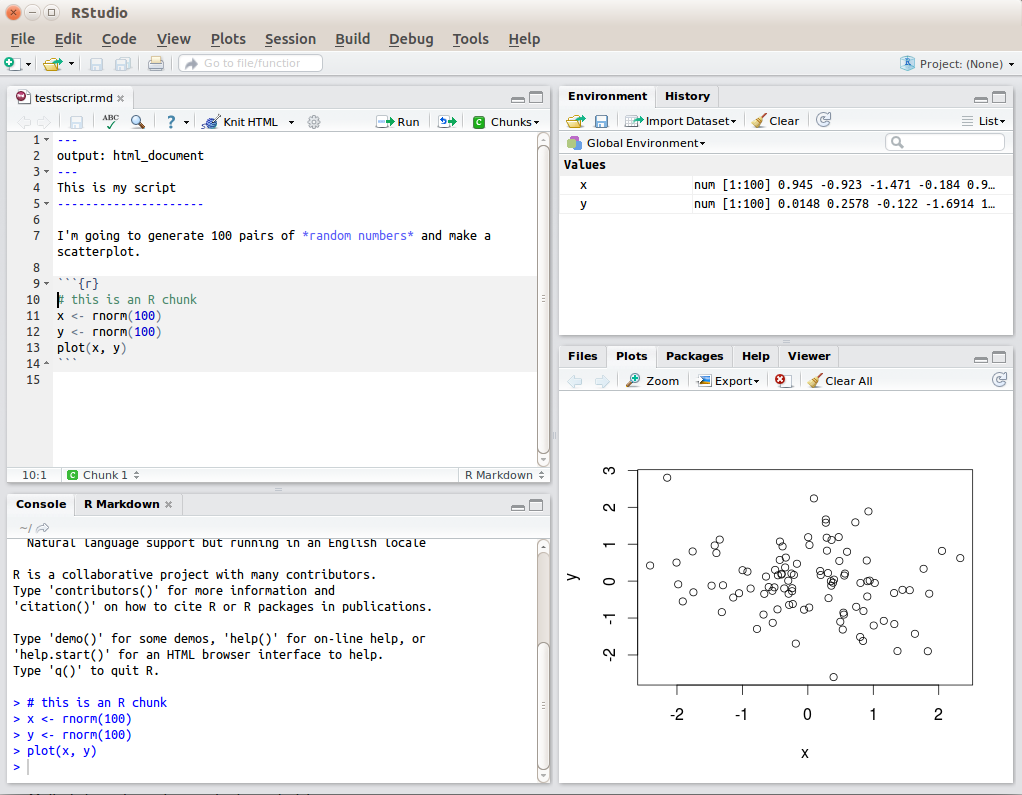
\includegraphics{https://github.com/BsoCool/UNSW-PSYC2001/blob/main/All%20images%20for%20computing%20tutorials/Introduction_to_R/RStudio.png?raw=true} 

}

\caption{RStudio interface}

\label{fig:img-rstudio}
\textbackslash end\{figure\}

\section{Functions and arguments}\label{functions-and-arguments}

\textbf{Functions} in R allow you to perform tasks that would take a long time to write out by hand, by only using one term! Think of them as nifty tools that will save you lots of typing, again and again. A function normally takes a number of \textbf{arguments} (you might want to think as these as verbs that require a subject and an object). You can look up all the arguments that a function takes by using the help documentation by using the format \texttt{?function}. Some arguments are required, and some are optional. Optional arguments will often use a default (normally specified in the help documentation) if you do not enter any value.

As an example, let's look at the help documentation for the function \texttt{rnorm()} which randomly generates a set of numbers with a normal distribution.

\section{Activity 1}\label{activity-1}

Open up R Studio and in the console, type the following code:

\begin{Shaded}
\begin{Highlighting}[]
\NormalTok{?rnorm}
\end{Highlighting}
\end{Shaded}

The help documentation for \texttt{rnorm()} should appear in the bottom right help panel. We know that the documentation for rnorm can be a little bit\ldots{} confusing. To simplify the \texttt{rnorm()} function is used to simulate data points from a normal distribution with a given mean and standard deviation. Do not worry about pnorm/dnorm, they can remain as mythical functions in the interest of simplicity.

In the usage section, we see that \texttt{rnorm()} takes the following form:

\begin{Shaded}
\begin{Highlighting}[]
\FunctionTok{rnorm}\NormalTok{(n, }\AttributeTok{mean =} \DecValTok{0}\NormalTok{, }\AttributeTok{sd =} \DecValTok{1}\NormalTok{)}
\end{Highlighting}
\end{Shaded}

In the arguments section, there are explanations for each of the arguments. \texttt{n} is the number of observations we want to create, \texttt{mean} is the mean of the data points we will create and \texttt{sd} is the standard deviation of the set. In the details section it notes that if no values are entered for \texttt{mean} and \texttt{sd} it will use a default of 0 and 1 for these values. Because there is no default value for \texttt{n} it must be specified otherwise the code won't run.

Let's try an example and just change the required argument \texttt{n} to ask R to produce 5 random numbers.

\section{Activity 2}\label{activity-2}

\begin{itemize}
\tightlist
\item
  Copy and paste the following code into the console.
\end{itemize}

\begin{Shaded}
\begin{Highlighting}[]
\FunctionTok{set.seed}\NormalTok{(}\DecValTok{12042016}\NormalTok{)}
\FunctionTok{rnorm}\NormalTok{(}\AttributeTok{n =} \DecValTok{5}\NormalTok{)}
\end{Highlighting}
\end{Shaded}

\begin{verbatim}
## [1] -0.2896163 -0.6428964  0.5829221 -0.3286728 -0.5110101
\end{verbatim}

These numbers have a mean of 0 and an SD of 1. Now we can change the additional arguments to produce a different set of numbers.

\begin{Shaded}
\begin{Highlighting}[]
\FunctionTok{rnorm}\NormalTok{(}\AttributeTok{n =} \DecValTok{5}\NormalTok{, }\AttributeTok{mean =} \DecValTok{10}\NormalTok{, }\AttributeTok{sd =} \DecValTok{2}\NormalTok{)}
\end{Highlighting}
\end{Shaded}

\begin{verbatim}
## [1] 13.320853  9.377956 10.235461  9.811793 13.019102
\end{verbatim}

This time R has still produced 5 random numbers, but now this set of numbers has a mean of 10 and an sd of 2 as specified. Always remember to use the help documentation to help you understand what arguments a function requires.

\section{Argument names}\label{argument-names}

In the above examples, we have written out the argument names in our code (e.g., \texttt{n}, \texttt{mean}, \texttt{sd}), however, this is not strictly necessary. The following two lines of code would both produce the same result (although each time you run \texttt{rnorm()} it will produce a slightly different set of numbers, because it's random, but they would still have the same mean and SD):

\begin{Shaded}
\begin{Highlighting}[]
\FunctionTok{rnorm}\NormalTok{(}\AttributeTok{n =} \DecValTok{6}\NormalTok{, }\AttributeTok{mean =} \DecValTok{3}\NormalTok{, }\AttributeTok{sd =} \DecValTok{1}\NormalTok{)}
\FunctionTok{rnorm}\NormalTok{(}\DecValTok{6}\NormalTok{, }\DecValTok{3}\NormalTok{, }\DecValTok{1}\NormalTok{)}
\end{Highlighting}
\end{Shaded}

Importantly, if you do not write out the argument names, R will use the default order of arguments, that is for \texttt{rnorm} it will assume that the first number you enter is \texttt{n}. the second number is \texttt{mean} and the third number is \texttt{sd}.

If you write out the argument names then you can write the arguments in whatever order you like:

\begin{Shaded}
\begin{Highlighting}[]
\FunctionTok{rnorm}\NormalTok{(}\AttributeTok{sd =} \DecValTok{1}\NormalTok{, }\AttributeTok{n =} \DecValTok{6}\NormalTok{, }\AttributeTok{mean =} \DecValTok{3}\NormalTok{)}
\end{Highlighting}
\end{Shaded}

When you are first learning R, you may find it useful to write out the argument names as it can help you remember and understand what each part of the function is doing. However, as your skills progress you may find it quicker to omit the argument names and you will also see examples of code online that do not use argument names so it is important to be able to understand which argument each bit of code is referring to (or look up the help documentation to check).

In this course, we will always write out the argument names the first time we use each function, however, in subsequent uses they may be omitted.

\section{Tab auto-complete}\label{tab-auto-complete}

One very useful feature of R Studio is the tab auto-complete for functions (\textbf{see Figure 2: Tab auto-complete}). If you write the name of the function and then press the tab key, R Studio will show you the arguments that function takes along with a brief description. If you press enter on the argument name it will fill in the name for you, just like auto-complete on your phone. This is incredibly useful when you are first learning R and you should remember to use this feature frequently.

\textbackslash begin\{figure\}

\{\centering 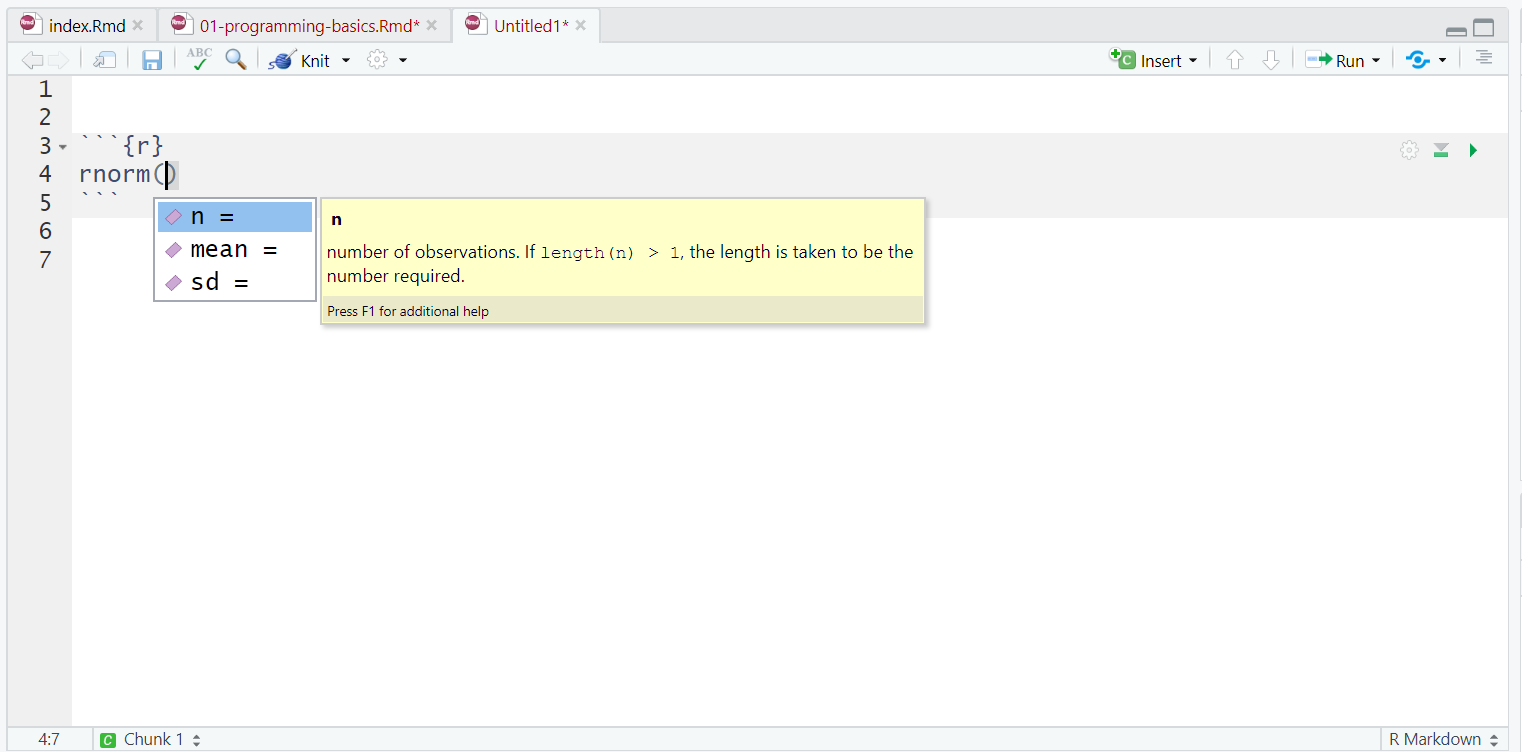
\includegraphics{https://github.com/BsoCool/UNSW-PSYC2001/blob/main/All%20images%20for%20computing%20tutorials/Introduction_to_R/autocomplete.png?raw=true} 

}

\caption{Tab auto-complete}

\label{fig:img-autocomplete}
\textbackslash end\{figure\}

\section{Base R and packages}\label{base-r-and-packages}

When you install R you will have access to a range of functions including options for data wrangling and statistical analysis. The functions that are included in the default installation are typically referred to as \textbf{Base R} and there is a useful cheat sheet that shows many Base R functions \href{https://stat.ethz.ch/R-manual/R-devel/library/base/html/00Index.html}{here}.

However, the power of R is that it is extendable and open source - put simply, if a function doesn't exist or doesn't work very well, anyone can create a new \textbf{package} that contains data and code to allow you to perform new tasks. You may find it useful to think of Base R as the default apps that come on your phone and packages as additional apps that you need to download separately.

\section{Installing and loading packages}\label{installing-and-loading-packages}

Info: The UNSW psychology computers will already have all of the packages you need for this course so you only need to install packages if you are using your own machine.

\section{Activity 3: Install the tidyverse}\label{activity-3-install-the-tidyverse}

In order to use a package, you must first install it. The following code installs the package \texttt{tidyverse}, a package we will use very frequently in this course.

If you are interested in learning more about tidyverse and how incredibly useful it is in R, please consider reading \href{https://r4ds.hadley.nz/}{R for Data Science}

\begin{itemize}
\tightlist
\item
  If you are working on your own computer, use the below code to install the tidyverse. \textbf{Do not do this if you are working on a University machine}.
\end{itemize}

\begin{Shaded}
\begin{Highlighting}[]
\FunctionTok{install.packages}\NormalTok{(}\StringTok{"tidyverse"}\NormalTok{)}
\end{Highlighting}
\end{Shaded}

You only need to install a package once, however, each time you start R you need to load the packages you want to use, in a similar way that you need to install an app on your phone once, but you need to open it every time you want to use it.

To load packages we use the function \texttt{library()}. Typically you would start any analysis script by loading all of the packages you need, but we will come back to that in the labs.

\section{Activity 4: Load the tidyverse}\label{activity-4-load-the-tidyverse}

\begin{itemize}
\tightlist
\item
  Run the below code to load the tidyverse. You can do this regardless of whether you are using your own computer or a University machine.
\end{itemize}

\begin{Shaded}
\begin{Highlighting}[]
\FunctionTok{library}\NormalTok{(tidyverse)}
\end{Highlighting}
\end{Shaded}

You will get what looks like an error message - it's not. It's just R telling you what it's done.

Now that we've loaded the \texttt{tidyverse} package we can use any of the functions it contains but remember, you need to run the \texttt{library()} function every time you start R.

\section{Package updates}\label{package-updates}

In addition to updates to R and R Studio, the creators of packages also sometimes update their code. This can be to add functions to a package, or it can be to fix errors. One thing to avoid is unintentionally updating an installed package. When you run \texttt{install.packages()} it will always install the latest version of the package and it will overwrite any older versions you may have installed. Sometimes this isn't a problem, however, sometimes you will find that the update means your code no longer works as the package has changed substantially. It is possible to revert back to an older version of a package but try to avoid this anyway.

Warning: To avoid accidentally overwriting a package with a later version, you should \textbf{never} include \texttt{install.packages()} in your analysis scripts in case you, or someone else runs the code by mistake. Remember, the UNSW psychology computers will already have all of the packages you need for this course so you only need to install packages if you are using your own machine.

\section{Package conflicts}\label{package-conflicts}

There are thousands of different R packages with even more functions. Unfortunately, sometimes different packages have the same function names. For example, the packages \texttt{dplyr} and \texttt{MASS} both have a function named \texttt{select()}. If you load both of these packages, R will produce a warning telling you that there is a conflict.

\begin{Shaded}
\begin{Highlighting}[]
\FunctionTok{library}\NormalTok{(dplyr)}
\end{Highlighting}
\end{Shaded}

\begin{verbatim}
## Warning: package 'dplyr' was built under R version 4.3.3
\end{verbatim}

\begin{verbatim}
## 
## Attaching package: 'dplyr'
\end{verbatim}

\begin{verbatim}
## The following objects are masked from 'package:stats':
## 
##     filter, lag
\end{verbatim}

\begin{verbatim}
## The following objects are masked from 'package:base':
## 
##     intersect, setdiff, setequal, union
\end{verbatim}

\begin{Shaded}
\begin{Highlighting}[]
\FunctionTok{library}\NormalTok{(MASS)}
\end{Highlighting}
\end{Shaded}

\begin{verbatim}
## 
## Attaching package: 'MASS'
\end{verbatim}

\begin{verbatim}
## The following object is masked from 'package:dplyr':
## 
##     select
\end{verbatim}

In this case, R is telling you that the function \texttt{select()} in the \texttt{dplyr} package is being hidden (or `masked') by another function with the same name. If you were to try and use \texttt{select()}, R would use the function from the package that was loaded most recently - in this case it would use the function from \texttt{MASS}.

If you want to specify which package you want to use for a particular function you can use code in the format \texttt{package::function}, for example:

\begin{Shaded}
\begin{Highlighting}[]
\NormalTok{dplyr}\SpecialCharTok{::}\FunctionTok{select}\NormalTok{()}
\NormalTok{MASS}\SpecialCharTok{::}\FunctionTok{select}\NormalTok{()}
\end{Highlighting}
\end{Shaded}

Note that this is for your own information, so that you aren't alarmed when you see such messages in your great future of data analysis. You won't have to worry about package conflicts during this course.

\section{Objects}\label{objects}

A large part of your coding for data analysis will involve creating and manipulating objects. Objects contain stuff. That stuff can be numbers, words, or the result of operations and analyses.You assign content to an object using \texttt{\textless{}-}.

\section{Activity 5: Create some objects}\label{activity-5-create-some-objects}

\begin{itemize}
\tightlist
\item
  Copy and paste the following code into the console, change the code so that it uses your own name and age and run it. You should see that \texttt{name}, \texttt{age}, \texttt{today}, \texttt{new\_year}, and \texttt{data} appear in the environment pane.
\end{itemize}

\begin{Shaded}
\begin{Highlighting}[]
\NormalTok{name }\OtherTok{\textless{}{-}} \StringTok{"emily"}
\NormalTok{age }\OtherTok{\textless{}{-}} \DecValTok{15} \SpecialCharTok{+} \DecValTok{18} 
\NormalTok{today }\OtherTok{\textless{}{-}}\FunctionTok{Sys.Date}\NormalTok{()}
\NormalTok{new\_year }\OtherTok{\textless{}{-}} \FunctionTok{as.Date}\NormalTok{(}\StringTok{"2020{-}01{-}01"}\NormalTok{)}
\NormalTok{data }\OtherTok{\textless{}{-}} \FunctionTok{rnorm}\NormalTok{(}\AttributeTok{n =} \DecValTok{10}\NormalTok{, }\AttributeTok{mean =} \DecValTok{15}\NormalTok{, }\AttributeTok{sd =} \DecValTok{3}\NormalTok{)}
\end{Highlighting}
\end{Shaded}

\textbackslash begin\{figure\}

\{\centering 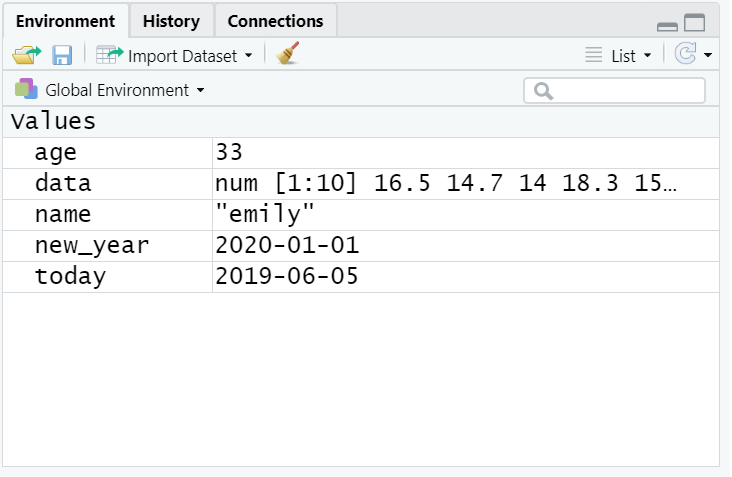
\includegraphics{https://github.com/BsoCool/UNSW-PSYC2001/blob/main/All%20images%20for%20computing%20tutorials/Introduction_to_R/objects-enviro.png?raw=true} 

}

\caption{Objects in the environment}

\label{fig:img-objects-enviro}
\textbackslash end\{figure\}

Note that in these examples, \texttt{name},\texttt{age}, and \texttt{new\_year} would always contain the values \texttt{emily}, \texttt{33}, and the date of New Year's Day 2020, however, \texttt{today} will draw the date from the operating system and \texttt{data} will be a randomly generated set of data so the values of these objects will not be static.

Warning: You may also see objects referred to as `variables'. There is a difference between the two in programming terms, however, they are used synonymously very frequently.

As a side note, if you ever have to teach programming and statistics, don't use your age as an example because everytime you have to update your teaching materials you get a reminder of the fragility of existence and your advancing age.

Importantly, objects can be involved in calculations and can interact with each other. For example:

\begin{Shaded}
\begin{Highlighting}[]
\NormalTok{age }\SpecialCharTok{+} \DecValTok{10}
\end{Highlighting}
\end{Shaded}

\begin{verbatim}
## [1] 43
\end{verbatim}

\begin{Shaded}
\begin{Highlighting}[]
\NormalTok{new\_year }\SpecialCharTok{{-}}\NormalTok{ today}
\end{Highlighting}
\end{Shaded}

\begin{verbatim}
## Time difference of -2070 days
\end{verbatim}

\begin{Shaded}
\begin{Highlighting}[]
\FunctionTok{mean}\NormalTok{(data)}
\end{Highlighting}
\end{Shaded}

\begin{verbatim}
## [1] 17.66644
\end{verbatim}

Finally, you can store the result of these operations in a new object:

\begin{Shaded}
\begin{Highlighting}[]
\NormalTok{decade }\OtherTok{\textless{}{-}}\NormalTok{ age }\SpecialCharTok{+} \DecValTok{10}
\end{Highlighting}
\end{Shaded}

Tip: You may find it helpful to read \texttt{\textless{}-} as \texttt{contains}, e.g., \texttt{name} contains the text \texttt{emily}.

\section{Datatypes}\label{datatypes}

You will constantly be creating objects throughout this course and you will learn more about them and how they behave as we go along, however, for now it is enough to understand that they are a way of saving values, that these values can be numbers, text, or the result of operations, and that they can be used in further operations to create new variables. For now, we can have a look at the datatypes of our objects using the function \texttt{typeof}.

\begin{Shaded}
\begin{Highlighting}[]
\CommentTok{\#These are both doubles (i.e numbers!)}
\FunctionTok{typeof}\NormalTok{(age)}
\end{Highlighting}
\end{Shaded}

\begin{verbatim}
## [1] "double"
\end{verbatim}

\begin{Shaded}
\begin{Highlighting}[]
\FunctionTok{typeof}\NormalTok{(new\_year)}
\end{Highlighting}
\end{Shaded}

\begin{verbatim}
## [1] "double"
\end{verbatim}

\begin{Shaded}
\begin{Highlighting}[]
\CommentTok{\#This is a chr (i.e contains letters!)}
\FunctionTok{typeof}\NormalTok{(name)}
\end{Highlighting}
\end{Shaded}

\begin{verbatim}
## [1] "character"
\end{verbatim}

Info: There are 5 main datatypes: double, integer, complex, logical and character. For historic reasons, double is also called numeric. We will learn about and use many of these different datatypes in this course.

We will learn about using these datatypes (as well as some of the others) throughout this course, so don't fret if you don't understand it yet !

\section{Looking after the environment}\label{looking-after-the-environment}

If you've been writing a lot of code you may find that the environment pane (or workspace) has become cluttered with many objects. This can make it difficult to figure out which object you need and therefore you run the risk of using the wrong data frame. If you're working on a new dataset, or if you've tried lots of different code before getting the final version, it is good practice to remember to clear the environment to avoid using the wrong object. You can do this in several way.

\begin{enumerate}
\def\labelenumi{\arabic{enumi}.}
\tightlist
\item
  To remove individual objects, you can type \texttt{rm(object\_name)} in the console. Try this now to remove one of the objects you created in the previous section.
\item
  To clear all objects from the environment run \texttt{rm(list\ =\ ls())} in the console.
\item
  To clear all objects from the environment you can also click the broom icon in the environment pane.
\end{enumerate}

\textbackslash begin\{figure\}

\{\centering 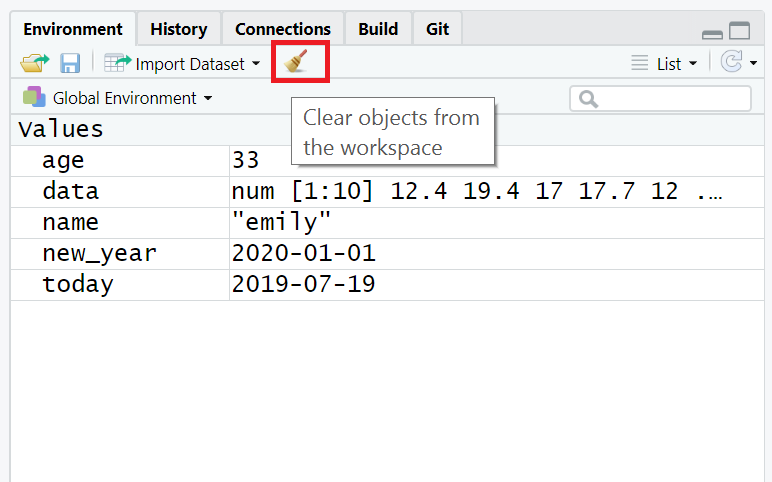
\includegraphics{https://github.com/BsoCool/UNSW-PSYC2001/blob/main/All%20images%20for%20computing%20tutorials/Introduction_to_R/broom.png?raw=true} 

}

\caption{Clearing the workspace}

\label{fig:unnamed-chunk-4}
\textbackslash end\{figure\}

\section{You are Free!}\label{you-are-free}

Congratulations you have survived the first tutorial for this course. We look forward to seeing you next week for more coding fun.

\textbackslash begin\{figure\}

\{\centering 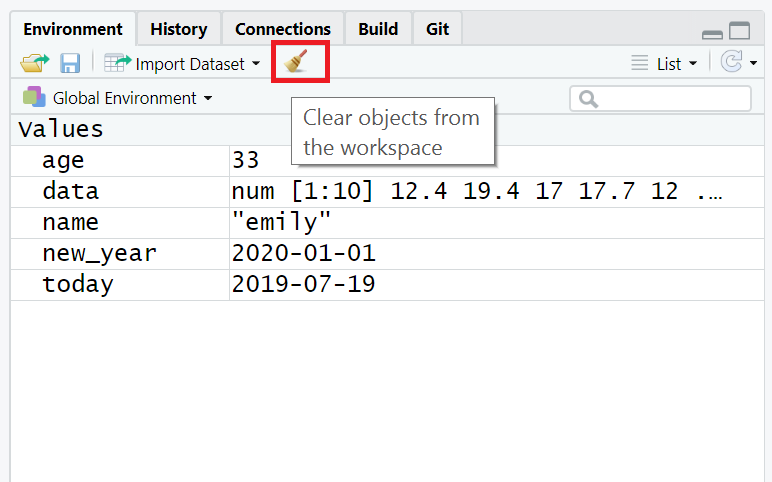
\includegraphics{https://github.com/BsoCool/UNSW-PSYC2001/blob/main/All%20images%20for%20computing%20tutorials/Introduction_to_R/broom.png?raw=true} 

}

\caption{Students reaction to finishing this}

\label{fig:unnamed-chunk-5}
\textbackslash end\{figure\}

\chapter{Data wrangling and visualisation}\label{data-wrangling-and-visualisation}

\section{Checking installation and loading packages}\label{checking-installation-and-loading-packages}

Before we can \textbf{begin} any script we first need to make sure that the \textbf{required packages are installed} in our version of RStudio. Next, we can \textbf{load the required packages} to be used in the script. The code block below will do this for you.

Note that in the code below, we've added a fancy \texttt{if} statement to check if the packages are installed. If they are not installed, it will install them for you. This is a good practice to ensure that your code runs smoothly on any computer without needing to manually install packages. Particularly if you are using the University's computers, where we have already installed the packages you need (and we ask you not to install any more!).

\begin{Shaded}
\begin{Highlighting}[]
\CommentTok{\# Check if packages are installed, if not install.}
\ControlFlowTok{if}\NormalTok{(}\SpecialCharTok{!}\FunctionTok{require}\NormalTok{(here)) }\FunctionTok{install.packages}\NormalTok{(}\StringTok{\textquotesingle{}here\textquotesingle{}}\NormalTok{) }\CommentTok{\#checks if a package is installed and installs it if required.}
\ControlFlowTok{if}\NormalTok{(}\SpecialCharTok{!}\FunctionTok{require}\NormalTok{(tidyverse)) }\FunctionTok{install.packages}\NormalTok{(}\StringTok{\textquotesingle{}tidyverse\textquotesingle{}}\NormalTok{)}
\ControlFlowTok{if}\NormalTok{(}\SpecialCharTok{!}\FunctionTok{require}\NormalTok{(ggplot2)) }\FunctionTok{install.packages}\NormalTok{(}\StringTok{\textquotesingle{}ggplot2\textquotesingle{}}\NormalTok{)}

\FunctionTok{library}\NormalTok{(here) }\CommentTok{\#loads in the specified package}
\FunctionTok{library}\NormalTok{(tidyverse)}
\FunctionTok{library}\NormalTok{(ggplot2)}
\end{Highlighting}
\end{Shaded}

\section{What do packages do?}\label{what-do-packages-do}

You should be able to see that we have installed and loaded \textbf{3 different packages}. Let's first go over the basics of what a package is. In its simplest terms, a \textbf{package is a toolbox} that someone has created for us in R that \textbf{makes our life easier}. These packages build on the basic code that comes with the R programming language (what \textbf{RStudio} uses to run), called \texttt{base\ R}.

\textbackslash begin\{figure\}

\{\centering \includegraphics[width=0.5\linewidth]{https://github.com/BsoCool/UNSW-PSYC2001/blob/main/All%20images%20for%20computing%20tutorials/Data_wrangling_and_visualization/Opening%20an%20R%20package.gif?raw=true} 

}

\caption{Opening an R package}

\label{fig:unnamed-chunk-7}
\textbackslash end\{figure\}

\section{What do these packages do?}\label{what-do-these-packages-do}

It is always a \textbf{good idea to check the documentation} for a package before you use it. We can do this by using the \textbf{help syntax}, which is the \texttt{?}. The package we are trying to get help with is called \texttt{here}. Try to run this code by \textbf{clicking on the green arrow on the corner of the code block on the left side of your screen}. This will open a webpage that tells us the \textbf{purpose} of the \texttt{here} package and how it works.

\textbackslash begin\{figure\}

\{\centering \includegraphics[width=1\linewidth]{https://github.com/BsoCool/UNSW-PSYC2001/blob/main/All%20images%20for%20computing%20tutorials/Data_wrangling_and_visualization/Example%20of%20running%20code.jpg?raw=true} 

}

\caption{Running code in R}

\label{fig:unnamed-chunk-8}
\textbackslash end\{figure\}

\begin{Shaded}
\begin{Highlighting}[]
\NormalTok{?here }\CommentTok{\#? loads the documentation for a specified package.}
\end{Highlighting}
\end{Shaded}

\section{Activity 1 - Using help syntax}\label{activity-1---using-help-syntax}

\textbf{Fill in the code block below} by putting in the \textbf{help syntax} \texttt{?} and the name of the package you are interested in. This will get the documentation for the \textbf{other packages} we are using. You can do this by substituting in the packages that we are using from above. Have a read of each of these pages and click on any links you find interesting. These are the \textbf{main packages} we will be using throughout this course.

\begin{Shaded}
\begin{Highlighting}[]
\CommentTok{\# Try to use the help function \textquotesingle{}?\textquotesingle{} to read more about the packages we are using today}
\CommentTok{\# The packages we are using are \textquotesingle{}tidyverse\textquotesingle{} and \textquotesingle{}ggplot2\textquotesingle{}.}

\NormalTok{?tidyverse}
\NormalTok{?ggplot2}
\end{Highlighting}
\end{Shaded}

\section{Organisation and CSV files}\label{organisation-and-csv-files}

The dataset we are using should be downloaded from the tutorial folder on Moodle. On your computer navigate to this folder and have a look at what it contains.

You should note that it contains the following:

\begin{itemize}
\tightlist
\item
  An R Project file called \textbf{`Data\_wrangling\_and\_visualization.Rproj'}
\item
  An R Markdown file called \textbf{`Data\_wrangling\_and\_visualization.Rmd'}.
\item
  A text file called \textbf{README.txt'}
\item
  A folder called \textbf{data}, containing a .csv file called \textbf{`PSYC2001\_social-media-data.csv'}
\item
  A folder called \textbf{output}, which is where all your output will go.
\item
  A folder called \textbf{scripts} which is where all new scripts will go.
\end{itemize}

These are the \textbf{key ingredients needed to organise all projects in R}.

\textbackslash begin\{figure\}

\{\centering \includegraphics[width=1\linewidth]{https://github.com/BsoCool/UNSW-PSYC2001/blob/main/All%20images%20for%20computing%20tutorials/Data_wrangling_and_visualization/Example%20of%20folder.JPG?raw=true} 

}

\caption{Project Organisation}

\label{fig:unnamed-chunk-11}
\textbackslash end\{figure\}

You will notice that the data for today, called \texttt{PSYC2001\_social-media-data.csv}, is a \textbf{csv file} (short for a \emph{Comma Separated Value} file).

csv files are a common and handy way to store data, because they can be read by heaps of different programs, like Excel, Google Sheets, and R. They are simple text files where each line represents a row of data, and the values in each row are separated by commas. Try double clicking on the csv file now to see what happens. You'll see that Excel offers to open it for you. Click ok to open the file in Excel and take a look at how the data looks. Then say `that's very kind of you Excel, but we are more powerful than you. We R.'

\textbackslash begin\{figure\}

\{\centering \includegraphics[width=1\linewidth]{https://github.com/BsoCool/UNSW-PSYC2001/blob/main/All%20images%20for%20computing%20tutorials/Data_wrangling_and_visualization/Data%20in%20excel.JPG?raw=true} 

}

\caption{Social Media Data in Excel}

\label{fig:unnamed-chunk-12}
\textbackslash end\{figure\}

\section{Importing your Data in R}\label{importing-your-data-in-r}

We are now going to load our first dataset into R. To do this we will need to \textbf{import the dataset} using a function capable of importing csv files.

We will be using \textbf{two different functions} to achieve this. The \texttt{read.csv()} function is used to import our csv dataset and it comes from the \texttt{utils} package which is part of \texttt{base\ R}. But the \texttt{read.csv()} function needs to know where the file lives on the computer. To do this, we use the \texttt{here()} function from the \texttt{here} package. This function tells R the \textbf{location of the project} we are working from, to make locating the data easier.

Let's first confirm that \texttt{here()} knows our current location on this PC (called the \textbf{`Working Directory'})

\begin{Shaded}
\begin{Highlighting}[]
\FunctionTok{here}\NormalTok{()}
\end{Highlighting}
\end{Shaded}

\begin{verbatim}
## [1] "G:/Current/Student folders/Bart Cool/Work/PSYC2001 in R/UNSW_PSYC2001-Bookdown - Copy/PSYC2001 Computing Coursebook"
\end{verbatim}

We can use this to easily find where our file is located and read it.

\begin{Shaded}
\begin{Highlighting}[]
\NormalTok{social\_media }\OtherTok{\textless{}{-}} \FunctionTok{read.csv}\NormalTok{(}\AttributeTok{file =} \FunctionTok{here}\NormalTok{(}\StringTok{"Data"}\NormalTok{,}\StringTok{"PSYC2001\_social{-}media{-}data.csv"}\NormalTok{)) }\CommentTok{\#reads in csv files}
\end{Highlighting}
\end{Shaded}

Note that this code works because `Data' is a folder in the same directory as the \texttt{.Rproj} file. If the folder Data was somewhere else, then using \texttt{here()} would not work. We would need to instead specify the full path to the file. If you are unsure what we mean by `file path' then please google it, google it now.

Warning: If you have an error, something has gone wrong---please ask your tutor for help!

\section{Having a look at our imported data}\label{having-a-look-at-our-imported-data}

Our data should now be \textbf{imported into R!}

Recall from the \texttt{README.txt} file (\textbf{make sure you read this}) that this dataset was collected as part of an experiment investigating social media use in young Australian adults. Sixty young adults answered questions about their \textbf{social media usage} as well as their \textbf{political attitudes}. Data about their \textbf{social media usage} (e.g., likes) was collected while they used their preferred platforms under various conditions.

The variables in the data are:

\begin{itemize}
\tightlist
\item
  \texttt{id} -- a unique identifier (S1--S60)
\item
  \texttt{age} -- age in years
\item
  \texttt{time\_on\_social} -- average hours/day on social media (self-report diary)
\item
  \texttt{urban} -- urban (1) or rural (2) area (based on postcode density)
  -\texttt{good\_mood\_likes} -- likes/10 min during a good mood (from platform + diary)
\item
  \texttt{bad\_mood\_likes} -- as above, but during bad mood
\item
  \texttt{followers} -- average number of followers across platforms
\end{itemize}

The next 3 columns are political attitude subscales:

\begin{itemize}
\tightlist
\item
  \texttt{informed} -- how politically informed they feel (e.g., read news daily)
\item
  \texttt{campaign} -- how much they engage in campaign-related discussion
\item
  \texttt{activism} -- involvement in activism (e.g., protests, petitions)
\end{itemize}

We should now check that we have \textbf{imported into Rstudio matches this description (and what we saw when we opened it in excel)}. There are a couple of ways to do this.

\begin{itemize}
\tightlist
\item
  The first way is to \textbf{manually click} through to the dataset. You can do this by:

  \begin{enumerate}
  \def\labelenumi{\arabic{enumi}.}
  \tightlist
  \item
    Clicking on \textbf{Environment} in the top right section of your screen.
  \item
    Clicking on \textbf{social\_media}.
  \item
    You should see a new tab pop up with the data in a \textbf{table-like format} (this is called a \textbf{dataframe}).
  \item
    Make sure that this new tab looks similar to what you saw when you opened Excel file.
  \end{enumerate}
\end{itemize}

\textbackslash begin\{figure\}

\{\centering \includegraphics[width=2\linewidth]{https://github.com/BsoCool/UNSW-PSYC2001/blob/main/All%20images%20for%20computing%20tutorials/Data_wrangling_and_visualization/Directing%20students%20to%20view%20data%20in%20R.gif?raw=true} 

}

\caption{Navigating to dataset}

\label{fig:unnamed-chunk-15}
\textbackslash end\{figure\}

\begin{itemize}
\tightlist
\item
  We can also do this \textbf{programmatically} using the code blocks below:
\end{itemize}

\begin{Shaded}
\begin{Highlighting}[]
\CommentTok{\# Method 1 {-} Type in the name of the object}
\NormalTok{social\_media}
\end{Highlighting}
\end{Shaded}

\begin{Shaded}
\begin{Highlighting}[]
\CommentTok{\# Method 2 {-} Use the View function}
\FunctionTok{View}\NormalTok{(social\_media) }\CommentTok{\#view automatically displays the dataset in a tab.}
\end{Highlighting}
\end{Shaded}

\begin{Shaded}
\begin{Highlighting}[]
\CommentTok{\# Method 3 {-} Use the head function}
\FunctionTok{head}\NormalTok{(social\_media) }\CommentTok{\#head displays the first 6 rows of each variable.}
\end{Highlighting}
\end{Shaded}

\begin{verbatim}
##   id  age time_on_social urban good_mood_likes bad_mood_likes followers
## 1 S1 15.2           3.06     1            22.8           46.5     173.3
## 2 S2 16.0           2.18     1            46.0           48.3     144.3
## 3 S3 16.8           1.92     1            50.8           46.1      76.5
## 4 S4 15.6           2.61     1            29.9           29.2     171.7
## 5 S5 17.1           3.24     1            37.1           52.4     109.5
## 6 S6 15.7           2.44     1            26.9           20.2     157.5
##   polit_informed polit_campaign polit_activism
## 1            2.3            3.2            3.6
## 2            1.6            2.2            2.6
## 3            1.9            2.7            3.0
## 4            1.6            2.3            2.6
## 5            2.0            2.9            3.3
## 6            2.4            3.4            3.9
\end{verbatim}

\begin{Shaded}
\begin{Highlighting}[]
\CommentTok{\# Method 4 {-} Use the str function}
\FunctionTok{str}\NormalTok{(social\_media) }\CommentTok{\#displays an overall summary of the object and variable structure.}
\end{Highlighting}
\end{Shaded}

\begin{verbatim}
## 'data.frame':    60 obs. of  10 variables:
##  $ id             : chr  "S1" "S2" "S3" "S4" ...
##  $ age            : num  15.2 16 16.8 15.6 17.1 15.7 19.7 18.6 19.6 15.5 ...
##  $ time_on_social : num  3.06 2.18 1.92 2.61 3.24 2.44 1.46 1.52 1.92 2.1 ...
##  $ urban          : int  1 1 1 1 1 1 1 1 1 1 ...
##  $ good_mood_likes: num  22.8 46 50.8 29.9 37.1 26.9 14.8 26 6.5 45.7 ...
##  $ bad_mood_likes : num  46.5 48.3 46.1 29.2 52.4 20.2 35.1 35.8 12.2 32.8 ...
##  $ followers      : num  173.3 144.3 76.5 171.7 109.5 ...
##  $ polit_informed : num  2.3 1.6 1.9 1.6 2 2.4 1.7 1.6 1.5 2.2 ...
##  $ polit_campaign : num  3.2 2.2 2.7 2.3 2.9 3.4 2.4 2.2 2.1 3.1 ...
##  $ polit_activism : num  3.6 2.6 3 2.6 3.3 3.9 2.7 2.6 2.4 3.5 ...
\end{verbatim}

You should now have a good idea of what \texttt{PSYC2001\_social-media.csv} looks like in RStudio. This should match what we saw in excel.

You will also notice that the last function, \texttt{str()}, displays a \textbf{summary} of the object. This includes:

\begin{itemize}
\tightlist
\item
  The \textbf{object type} (a \textbf{dataframe})
\item
  The \textbf{number of observations/rows} (60)
\item
  The \textbf{number of variables/columns} (10)
\item
  The \textbf{datatype}: \textbf{chr} for \textbf{\texttt{id}}, and \textbf{num} for all other variables
\end{itemize}

Question: Please discuss with your deskmate and tutor what you think \textbf{chr} and \textbf{num} mean.

\textbackslash begin\{figure\}

\{\centering \includegraphics[width=0.5\linewidth]{https://github.com/BsoCool/UNSW-PSYC2001/blob/main/All%20images%20for%20computing%20tutorials/Data_wrangling_and_visualization/Students%20thinking.gif?raw=true} 

}

\caption{You thinking}

\label{fig:unnamed-chunk-20}
\textbackslash end\{figure\}

\section{Checking the quality of our data}\label{checking-the-quality-of-our-data}

Once we have imported our dataset into R, it's important to check the quality of the data. One simple way to do this is by using the \texttt{summary()} function.

\begin{Shaded}
\begin{Highlighting}[]
\FunctionTok{summary}\NormalTok{(social\_media) }\CommentTok{\#summary provides a quick overview of the data in each variable. }
\end{Highlighting}
\end{Shaded}

\begin{verbatim}
##       id                 age        time_on_social         urban    
##  Length:60          Min.   :13.90   Min.   :-999.000   Min.   :1.0  
##  Class :character   1st Qu.:15.70   1st Qu.:   1.920   1st Qu.:1.0  
##  Mode  :character   Median :16.50   Median :   2.365   Median :1.5  
##                     Mean   :16.87   Mean   : -30.845   Mean   :1.5  
##                     3rd Qu.:17.43   3rd Qu.:   3.042   3rd Qu.:2.0  
##                     Max.   :23.00   Max.   :   4.320   Max.   :2.0  
##  good_mood_likes bad_mood_likes    followers      polit_informed 
##  Min.   : 6.50   Min.   :12.20   Min.   : 61.40   Min.   :0.600  
##  1st Qu.:31.60   1st Qu.:39.08   1st Qu.: 76.47   1st Qu.:1.500  
##  Median :45.90   Median :49.30   Median :116.30   Median :1.800  
##  Mean   :43.04   Mean   :49.84   Mean   :124.76   Mean   :1.858  
##  3rd Qu.:53.40   3rd Qu.:58.75   3rd Qu.:153.75   3rd Qu.:2.200  
##  Max.   :89.20   Max.   :91.20   Max.   :336.50   Max.   :3.400  
##  polit_campaign  polit_activism 
##  Min.   :0.800   Min.   :0.900  
##  1st Qu.:2.100   1st Qu.:2.400  
##  Median :2.550   Median :2.900  
##  Mean   :2.602   Mean   :2.977  
##  3rd Qu.:3.100   3rd Qu.:3.500  
##  Max.   :4.800   Max.   :5.500
\end{verbatim}

Question: Do you notice anything unusual in the output of this data ? Discuss with your neighbour and tutor.

Hint: Take a closer look at the \texttt{time\_on\_social} variable.

\section{Cleaning the data}\label{cleaning-the-data}

It should now be clear that this data is unusual because it has a \textbf{minimum value} of \texttt{-999} in the \texttt{time\_on\_social} variable which is measured in hours (we can't have negative time !).

\textbackslash begin\{figure\}

\{\centering \includegraphics[width=0.5\linewidth]{https://github.com/BsoCool/UNSW-PSYC2001/blob/main/All%20images%20for%20computing%20tutorials/Data_wrangling_and_visualization/Back%20To%20The%20Future%20GIF.gif?raw=true} 

}

\caption{Back to the future !}

\label{fig:unnamed-chunk-22}
\textbackslash end\{figure\}

A good question to ask now is - \textbf{why are these values in the dataset?}

Sometimes when collecting data, we can't get a response from every participant. Instead of leaving a blank, researchers will sometimes put in a placeholder value like \texttt{-999} to show that the data is missing. These aren't real numbers; they just mean the data wasn't recorded. But \texttt{-999} isn't the standard way to show missing data in R. R uses \texttt{NA} to represent missing values, and that's important because most R functions know how to handle \texttt{NA} properly but they don't know to ignore \texttt{-999}.

Lets first have a look at how many \texttt{-999} values are present in the data. We can do this by using the \texttt{filter()} function from the \texttt{tidyverse} package which is used to keep (or remove) rows based on certain conditions.

\begin{Shaded}
\begin{Highlighting}[]
\NormalTok{social\_media\_filtered }\OtherTok{\textless{}{-}} \FunctionTok{filter}\NormalTok{(social\_media, time\_on\_social }\SpecialCharTok{==} \SpecialCharTok{{-}}\DecValTok{999}\NormalTok{) }\CommentTok{\#keep all rows where \textasciigrave{}time\_on\_social\textasciigrave{} is equal to {-}999}
\FunctionTok{View}\NormalTok{(social\_media\_filtered) }\CommentTok{\#view the filtered dataframe}
\end{Highlighting}
\end{Shaded}

Handily, we can then use the \texttt{count()} function from the \texttt{tidyverse} package to sum the number of rows in the resulting dataframe.

\begin{Shaded}
\begin{Highlighting}[]
\FunctionTok{count}\NormalTok{(social\_media\_filtered) }\CommentTok{\#count the number of rows in the filtered dataframe)}
\end{Highlighting}
\end{Shaded}

\begin{verbatim}
##   n
## 1 2
\end{verbatim}

\section{Introducing Piping}\label{introducing-piping}

A short aside to introduce a \textbf{very specical operation called a `pipe'} or \texttt{\%\textgreater{}\%}. This operation is part of the \texttt{tidyverse} package and allows you to pass the result from one function to the next seamlessly in a sort of assembly-line like fashion. \textbf{Throughout the rest of the course we will be using `piping' as it is easier to follow and code}. For instance, lets repeat what we just did above but with pipes instead.

\begin{Shaded}
\begin{Highlighting}[]
\NormalTok{social\_media }\SpecialCharTok{\%\textgreater{}\%} \CommentTok{\#pass the values from social\_media to the filter function}
  \FunctionTok{filter}\NormalTok{(time\_on\_social }\SpecialCharTok{==} \SpecialCharTok{{-}}\DecValTok{999}\NormalTok{) }\SpecialCharTok{\%\textgreater{}\%} \CommentTok{\#keep all rows that are equal to {-}999 and pass the result to count}
  \FunctionTok{count}\NormalTok{() }\CommentTok{\#count the number of remaining columns}
\end{Highlighting}
\end{Shaded}

\begin{verbatim}
##   n
## 1 2
\end{verbatim}

Info: Piping is not friends with every function. Some functions will not accept inputs from pipes (no matter how nice they are !). This will become clearer as we code throughout this course.

Now lets use a piping method to clean this data up by replacing \texttt{-999} values with more R readable \texttt{NA} values. \texttt{NA} stands for `Not Available' and is the standard way to represent missing data in R. We can do this using the \texttt{mutate()} and \texttt{na\_if()} functions from the \texttt{tidyverse} package. The \texttt{mutate()} function is used to alter or make new columns in a dataframe based on the conditions we specify and \texttt{na\_if()} is used to replace given values with \texttt{NA} in a dataframe.

\begin{Shaded}
\begin{Highlighting}[]
\NormalTok{social\_media\_NA }\OtherTok{\textless{}{-}}\NormalTok{ social\_media }\SpecialCharTok{\%\textgreater{}\%}
  \FunctionTok{mutate}\NormalTok{(}\AttributeTok{time\_on\_social =} \FunctionTok{na\_if}\NormalTok{(time\_on\_social,}\SpecialCharTok{{-}}\DecValTok{999}\NormalTok{)) }\CommentTok{\#mutate alters columns and rows. na\_if replaces {-}999 with NA}
\end{Highlighting}
\end{Shaded}

\section{Exporting Data}\label{exporting-data}

It would be a good idea to save this dataset for future tutorials, so that we don't have to replace \texttt{-999} values with \texttt{NA} values every single time.

We can do this with the \texttt{write.csv()} function from \texttt{baseR}. This function takes a dataframe in R and saves it as a .csv file on your computer. Later, we can simply read that csv back into R, and it will already be cleaned.

\begin{Shaded}
\begin{Highlighting}[]
\FunctionTok{write.csv}\NormalTok{(social\_media\_NA, }\FunctionTok{here}\NormalTok{(}\StringTok{"Output"}\NormalTok{,}\StringTok{"PSYC2001\_social{-}media{-}data{-}cleaned.csv"}\NormalTok{)) }\CommentTok{\#creates a csv file from the dataframe social\_media\_NA}
\end{Highlighting}
\end{Shaded}

\section{\texorpdfstring{Data visualization using \texttt{ggplot2}}{Data visualization using ggplot2}}\label{data-visualization-using-ggplot2}

Visualizing data is a crucial step in data analysis. You should never run a statistical analysis without first visualising your data. It helps us understand the distribution of our data, identify patterns, and communicate our findings effectively. It also helps us identify whether the data is suitable for the analysis we want to perform, or whether some weird values remain that could influence the result of our statistical tests, and even worse, our interpretations!

So, let's look at some data! We're going to start by visualising the \texttt{time\_on\_social} variable.

To do this we will need to use the \texttt{ggplot()} function. This is the main function from the \texttt{ggplot2} package (\textbf{you should know what this is from reading the documentation}). \texttt{ggplot()} provides the canvas of the graph you want to make.
To make the basic canvas \texttt{ggplot()} requires two things:

\begin{enumerate}
\def\labelenumi{\arabic{enumi}.}
\item
  The data that you want it to plot.
\item
  The variables to go on the x and y axes.
\end{enumerate}

Importantly, \texttt{ggplot()} only provides the canvas. It does not draw anything by itself. You have to add layers to the canvas created by \texttt{ggplot()} by using other functions that can create bars, points or lines !

Here we use \texttt{geom\_boxplot()} which creates a boxplot for us. What is a boxplot you ask ? A boxplot is a graph that shows the spread of data points where the lower part of the ``box'' represents the bottom quartile (where 25\% of the data lies), the upper part of the box represents the upper quartile (where 75\% of the data lies) and the middle of the box represents the median (the middle value). The ``whiskers'' (vertical lines) extend to the smallest and largest values not considered outliters.

\begin{Shaded}
\begin{Highlighting}[]
\NormalTok{social\_media\_NA }\SpecialCharTok{\%\textgreater{}\%}
\FunctionTok{ggplot}\NormalTok{(}\FunctionTok{aes}\NormalTok{(}\AttributeTok{y =}\NormalTok{ time\_on\_social),) }\SpecialCharTok{+} \CommentTok{\#ggplot uses aesthetic (aes()) to map axes. }
  \FunctionTok{scale\_x\_discrete}\NormalTok{() }\SpecialCharTok{+} \CommentTok{\#this tells ggplot that the x{-}axis is categorical.}
  \FunctionTok{geom\_boxplot}\NormalTok{() }\SpecialCharTok{+} \CommentTok{\#creates a boxplot}
  \FunctionTok{labs}\NormalTok{(}\AttributeTok{y =} \StringTok{"Time on Social Media"}\NormalTok{) }\CommentTok{\#short for "labels", use to label axes and titles.}
\end{Highlighting}
\end{Shaded}

\begin{verbatim}
## Warning: Removed 2 rows containing non-finite outside the scale range
## (`stat_boxplot()`).
\end{verbatim}

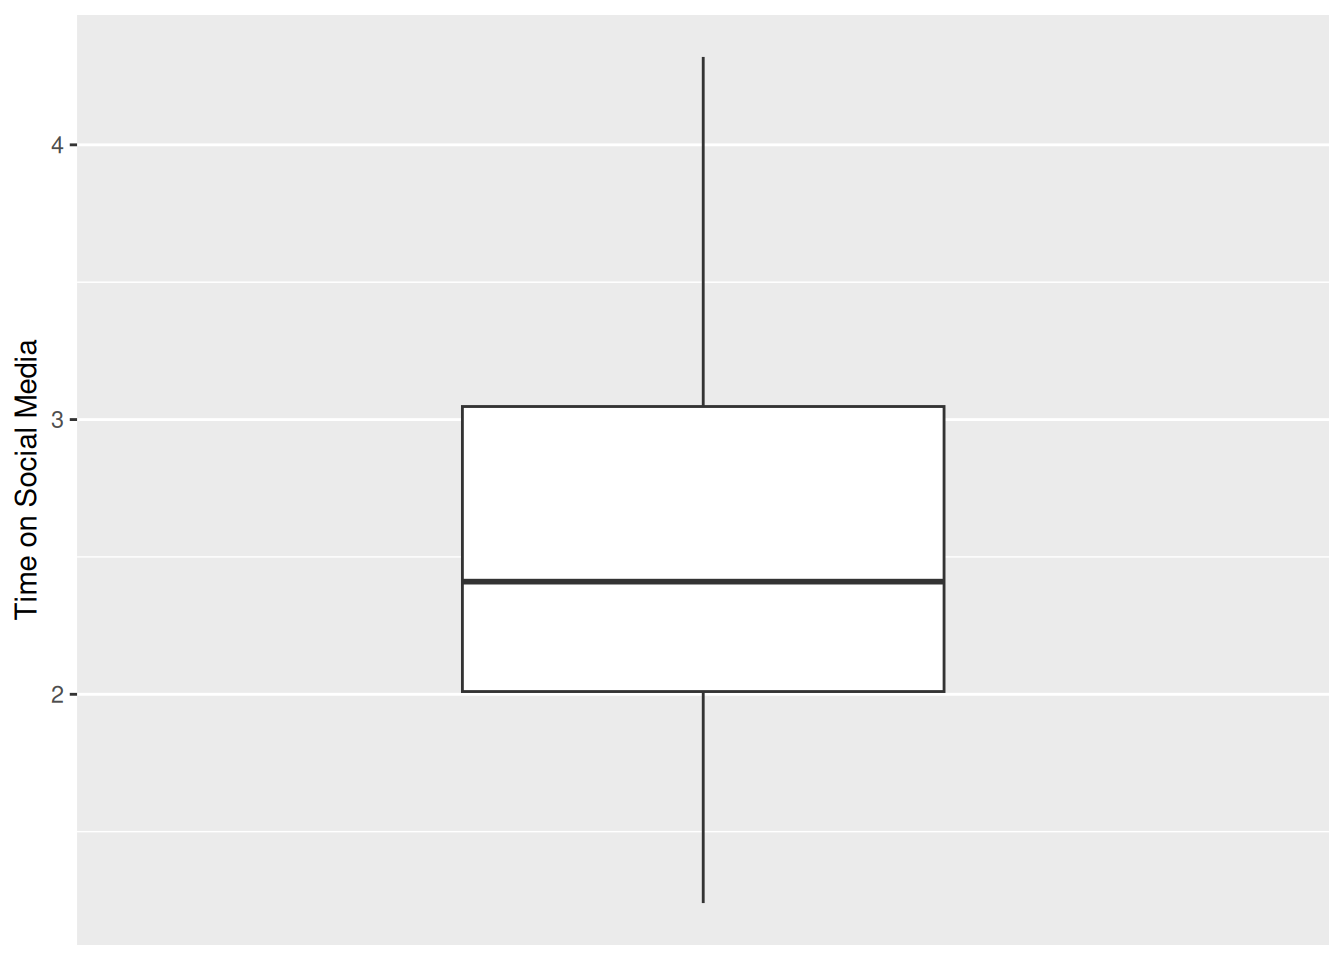
\includegraphics{_main_files/figure-latex/unnamed-chunk-24-1.pdf}

Warning: We receive a warning here because \texttt{ggplot()} is able to recognise and remove `NA' values. Be \textbf{careful} as not all R functions are able to do this.

Question: What approximately is the median value? The lower quartile? The upper quartile? Is there another way that we could get this information in a more exact form ? Discuss this with your deskmate and your tutor.

\section{\texorpdfstring{Activity 2 - Creating a histogram in \texttt{ggplot()}}{Activity 2 - Creating a histogram in ggplot()}}\label{activity-2---creating-a-histogram-in-ggplot}

\texttt{ggplot()} can be customised with so many other functions that we have shown here to make truly \href{https://r-graph-gallery.com/ggplot2-package.html}{beautiful looking plots}. We will be learning how to do this throughout the next few weeks.

For now lets see if you can put some of the skills you have learned so far to good use. See if you can work out how to make a histogram of the data using the function \texttt{geom\_histogram()}

Hint: You will only need to provide an x variable this time !

\begin{Shaded}
\begin{Highlighting}[]
\NormalTok{social\_media\_NA }\SpecialCharTok{\%\textgreater{}\%}
\FunctionTok{ggplot}\NormalTok{(}\FunctionTok{aes}\NormalTok{(}\AttributeTok{x =}\NormalTok{ time\_on\_social)) }\SpecialCharTok{+} \CommentTok{\#ggplot uses aesthetic (aes()) to map axes. }
  \FunctionTok{geom\_histogram}\NormalTok{() }\SpecialCharTok{+} \CommentTok{\#creates a histogram}
  \FunctionTok{labs}\NormalTok{(}\AttributeTok{x =} \StringTok{"Time on social media"}\NormalTok{, }\AttributeTok{y =} \StringTok{"Density"}\NormalTok{) }\CommentTok{\#short for "labels", use to label axes and titles.}
\end{Highlighting}
\end{Shaded}

::: \{style=``border-left: 4px solid \#9C27B0; background-color: \#F3E5F5; padding: 10px; margin: 10px 0;''\}
Question: What conclusions would you draw about the shape of the data, given your histogram? Please discuss with your deskmate and tutor.

\section{You are Free!}\label{you-are-free-1}

Well done ! You have completed everything you need to for this week. If you have finished in a record time please consult with your tutor about what to do next. Otherwise we will see you next lab !

\begin{figure}

{\centering 
\includegraphics[width=0.5\linewidth]{https://en.meming.world/images/en/5/5a/Ight_Imma_Head_Out} 

}

\caption{Students reaction to this information.}\label{fig:unnamed-chunk-26}
\end{figure}

\chapter{What is the sampling distribution of the mean}\label{what-is-the-sampling-distribution-of-the-mean}

\section{Checking installation and loading packages}\label{checking-installation-and-loading-packages-1}

As usual we first always check and load in our required packages.

\begin{Shaded}
\begin{Highlighting}[]
\CommentTok{\# Check if packages are installed, if not install.}
\ControlFlowTok{if}\NormalTok{(}\SpecialCharTok{!}\FunctionTok{require}\NormalTok{(here)) }\FunctionTok{install.packages}\NormalTok{(}\StringTok{\textquotesingle{}here\textquotesingle{}}\NormalTok{) }\CommentTok{\#checks if a package is installed and installs it if required.}
\ControlFlowTok{if}\NormalTok{(}\SpecialCharTok{!}\FunctionTok{require}\NormalTok{(tidyverse)) }\FunctionTok{install.packages}\NormalTok{(}\StringTok{\textquotesingle{}tidyverse\textquotesingle{}}\NormalTok{)}
\ControlFlowTok{if}\NormalTok{(}\SpecialCharTok{!}\FunctionTok{require}\NormalTok{(ggplot2)) }\FunctionTok{install.packages}\NormalTok{(}\StringTok{\textquotesingle{}ggplot2\textquotesingle{}}\NormalTok{)}

\FunctionTok{library}\NormalTok{(here) }\CommentTok{\#loads in the specified package}
\FunctionTok{library}\NormalTok{(tidyverse)}
\FunctionTok{library}\NormalTok{(ggplot2)}
\end{Highlighting}
\end{Shaded}

\section{Sampling distribution of the mean}\label{sampling-distribution-of-the-mean}

This week we will be learning a lot about the sampling distribution of the mean.

In last weeks lab you were introduced to a dataset looking at social media use in young adults. That data comes from a research programme run here at UNSW. However, this experiment has been repeated at 500 universities across the world, to get an in-depth global understanding of social media use in young adults.

Today you are going to look at your dataset from the last computing lab, and the data from across 500 universities. We will learn about the sampling distribution of the mean using the \texttt{time\_on\_social} variable. Remember, that this variables stands for the following:

\begin{itemize}
\tightlist
\item
  \texttt{time\_on\_social} -- average hours/day on social media (self-report diary)
\end{itemize}

\section{\texorpdfstring{Checking the mean of \texttt{time\_on\_social} from last week}{Checking the mean of time\_on\_social from last week}}\label{checking-the-mean-of-time_on_social-from-last-week}

First we want to have another look at the \texttt{PSYC2001\_social-media-data-cleaned.csv} dataset that we generated from last week. This dataset is `clean' because we converted all \texttt{-999} values to \texttt{NA}. We can first load it in using the same\texttt{read.csv()} function combined with \texttt{here()}.

\begin{Shaded}
\begin{Highlighting}[]
\NormalTok{social\_media }\OtherTok{\textless{}{-}} \FunctionTok{read.csv}\NormalTok{(}\AttributeTok{file =} \FunctionTok{here}\NormalTok{(}\StringTok{"Data"}\NormalTok{,}\StringTok{"PSYC2001\_social{-}media{-}data{-}cleaned.csv"}\NormalTok{)) }\CommentTok{\#reads in CSV files}
\end{Highlighting}
\end{Shaded}

Next we want to look at the mean of the variable \texttt{time\_on\_social}. This time since we have imported the clean version all we need to do is use the \texttt{summary()} function. Can you help with this ?

\begin{Shaded}
\begin{Highlighting}[]
\FunctionTok{summary}\NormalTok{(social\_media) }\CommentTok{\#provides a summary of all variables in the data. }
\end{Highlighting}
\end{Shaded}

\begin{verbatim}
##        X              id                 age        time_on_social 
##  Min.   : 1.00   Length:60          Min.   :13.90   Min.   :1.240  
##  1st Qu.:15.75   Class :character   1st Qu.:15.70   1st Qu.:2.010  
##  Median :30.50   Mode  :character   Median :16.50   Median :2.410  
##  Mean   :30.50                      Mean   :16.87   Mean   :2.539  
##  3rd Qu.:45.25                      3rd Qu.:17.43   3rd Qu.:3.047  
##  Max.   :60.00                      Max.   :23.00   Max.   :4.320  
##                                                     NA's   :2      
##      urban     good_mood_likes bad_mood_likes    followers      polit_informed 
##  Min.   :1.0   Min.   : 6.50   Min.   :12.20   Min.   : 61.40   Min.   :0.600  
##  1st Qu.:1.0   1st Qu.:31.60   1st Qu.:39.08   1st Qu.: 76.47   1st Qu.:1.500  
##  Median :1.5   Median :45.90   Median :49.30   Median :116.30   Median :1.800  
##  Mean   :1.5   Mean   :43.04   Mean   :49.84   Mean   :124.76   Mean   :1.858  
##  3rd Qu.:2.0   3rd Qu.:53.40   3rd Qu.:58.75   3rd Qu.:153.75   3rd Qu.:2.200  
##  Max.   :2.0   Max.   :89.20   Max.   :91.20   Max.   :336.50   Max.   :3.400  
##                                                                                
##  polit_campaign  polit_activism 
##  Min.   :0.800   Min.   :0.900  
##  1st Qu.:2.100   1st Qu.:2.400  
##  Median :2.550   Median :2.900  
##  Mean   :2.602   Mean   :2.977  
##  3rd Qu.:3.100   3rd Qu.:3.500  
##  Max.   :4.800   Max.   :5.500  
## 
\end{verbatim}

Question: What is the mean of \texttt{time\_on\_social} ?

\textbackslash begin\{figure\}

\{\centering \includegraphics[width=0.5\linewidth]{https://github.com/BsoCool/UNSW-PSYC2001/blob/main/All%20images%20for%20computing%20tutorials/What_is_the_sampling_distribution_of_the_mean/Deja%20Vu.jpg?raw=true} 

}

\caption{Deja Vu}

\label{fig:unnamed-chunk-29}
\textbackslash end\{figure\}

Now we are going to start looking at the new dataset for this week.

Info: All the information about this data and its variables are located in the \texttt{README.txt} file. If you have \textbf{NOT} read this yet please make sure you do !

\section{Activity 1 - Reading in Data}\label{activity-1---reading-in-data}

We are now going to read the dataset that we need for this week into R. The dataset can be read into an object called \texttt{global\_social\_media}. Please use the \texttt{read.csv()} and \texttt{here()} functions to read in the \texttt{PSYC2001\_global-time-on-social-data.csv} file in the code block below.

\begin{Shaded}
\begin{Highlighting}[]
\CommentTok{\#Use the read.csv() and here() functions to read in the dataset.}

\NormalTok{global\_social\_media }\OtherTok{\textless{}{-}} \FunctionTok{read.csv}\NormalTok{(}\AttributeTok{file =} \FunctionTok{here}\NormalTok{(}\StringTok{"Data"}\NormalTok{,}\StringTok{"PSYC2001\_global{-}time{-}on{-}social{-}data.csv"}\NormalTok{)) }\CommentTok{\#your code goes here}
\end{Highlighting}
\end{Shaded}

\section{Checking the UNSW value in this dataset.}\label{checking-the-unsw-value-in-this-dataset.}

Now, lets check whether the UNSW value (reminder this is \texttt{U49} from the \texttt{README.txt} file!) matches the mean value we had from the first week.

This should be pretty easy to do, and makes use of the \texttt{filter()} function we used \hyperref[cleaning-the-data]{last week}. This function is able to filter rows in your dataset that match a certain condition.

\begin{Shaded}
\begin{Highlighting}[]
\NormalTok{global\_social\_media }\SpecialCharTok{\%\textgreater{}\%} 
  \FunctionTok{filter}\NormalTok{(uni\_id }\SpecialCharTok{==} \StringTok{"U49"}\NormalTok{) }\CommentTok{\# reminder filter is used to select rows based on given conditions}
\end{Highlighting}
\end{Shaded}

\begin{verbatim}
##   uni_id mean_time_on_social
## 1    U49                2.54
\end{verbatim}

Yay ! The output should match the mean of what we calculated last week. This is because each value in the new data file is the mean value for the \texttt{time\_on\_social} variable, for each of the 500 experiments run (U1-U500), i.e.~the data contains 500 samples of the mean for \texttt{time\_on\_social}. This dataset is the result of repeating a single experiment, many times.

\section{Activity 2 - Finding the University of Sydney}\label{activity-2---finding-the-university-of-sydney}

Can you find the value for the University of Sydney (reminder this is \texttt{U102} from the \texttt{README.txt} file!) using the \texttt{filter()} function ?

\begin{Shaded}
\begin{Highlighting}[]
\NormalTok{global\_social\_media }\SpecialCharTok{\%\textgreater{}\%} 
  \FunctionTok{filter}\NormalTok{(uni\_id }\SpecialCharTok{==} \StringTok{"U102"}\NormalTok{)}
\end{Highlighting}
\end{Shaded}

\begin{verbatim}
##   uni_id mean_time_on_social
## 1   U102                2.68
\end{verbatim}

\section{Vectors and the sample function}\label{vectors-and-the-sample-function}

We are now going to have a look at what happens to the sampling distribution of the mean as we increase the number of mean samples in our samples (confusing I know !)

To do this we are going to make use of the \texttt{sample()} function from \texttt{baseR}. Lets first have a look at what this function does by using the \texttt{?} syntax. Please run the code block below:

\begin{Shaded}
\begin{Highlighting}[]
\NormalTok{?sample}
\end{Highlighting}
\end{Shaded}

In essence the \texttt{sample()} function randomly selects values from a vector. Since this function takes a vector as its first argument we we cannot just give it the entire dataframe as it does not know what to do with it. This will result in an error.

\begin{Shaded}
\begin{Highlighting}[]
\FunctionTok{sample}\NormalTok{(global\_social\_media, }\AttributeTok{size =} \DecValTok{10}\NormalTok{)}
\end{Highlighting}
\end{Shaded}

\begin{verbatim}
## Error in sample.int(length(x), size, replace, prob): cannot take a sample larger than the population when 'replace = FALSE'
\end{verbatim}

But you may be asking now, what is a vector? You can think of a vector as a single column in our dataframe. In this instance above, since the function only takes a single column, it gets overwhelmed when we pass it the entire dataframe. Poor function !

\textbackslash begin\{figure\}

\{\centering \includegraphics[width=0.5\linewidth]{https://github.com/BsoCool/UNSW-PSYC2001/blob/main/All%20images%20for%20computing%20tutorials/What_is_the_sampling_distribution_of_the_mean/Specter%20on%20a%20vector.jpg?raw=true} 

}

\caption{Specter on a Vector}

\label{fig:unnamed-chunk-34}
\textbackslash end\{figure\}

So we need to pass it only a single column. We can do this by using the \texttt{\$} operator from \texttt{baseR}. In essence the \texttt{\$} operator extracts a specified column from our dataframe.

Lets have a go at using it below:

\begin{Shaded}
\begin{Highlighting}[]
\FunctionTok{head}\NormalTok{(global\_social\_media}\SpecialCharTok{$}\NormalTok{uni\_id) }\CommentTok{\#head displays the first 6 elements. $ has been used to extract only the column uni\_id}
\end{Highlighting}
\end{Shaded}

\begin{verbatim}
## [1] "U1" "U2" "U3" "U4" "U5" "U6"
\end{verbatim}

You can see that this has lead to only the column \texttt{uni\_id} being extracted and shown in the function \texttt{head()}.

\section{What does the sampling distribution of the mean look like with only a few samples ?}\label{what-does-the-sampling-distribution-of-the-mean-look-like-with-only-a-few-samples}

Great ! So we now know how to pass a vector (column) into the \texttt{sample()} function. First lets try extracting a low number of samples, say 20 samples.

\begin{Shaded}
\begin{Highlighting}[]
\FunctionTok{set.seed}\NormalTok{(}\DecValTok{1}\NormalTok{) }\CommentTok{\#ensures we always get the same result from sampling ! }

\NormalTok{mean\_sample\_20 }\OtherTok{\textless{}{-}} \FunctionTok{sample}\NormalTok{(global\_social\_media}\SpecialCharTok{$}\NormalTok{mean\_time\_on\_social, }\AttributeTok{size =} \DecValTok{20}\NormalTok{) }\CommentTok{\#randomly samples 20 data points from mean\_time\_on\_social}

\NormalTok{mean\_sample\_20}
\end{Highlighting}
\end{Shaded}

\begin{verbatim}
##  [1] 3.08 1.56 1.82 2.31 3.07 3.48 2.42 2.90 1.90 2.45 3.07 2.31 2.00 2.02 2.31
## [16] 1.75 2.36 3.21 2.35 2.23
\end{verbatim}

Info: You might notice we use the \texttt{set.seed()} function. The purpose of this is to create reproducible results from randomness. You can go \href{https://www.statology.org/set-seed-in-r/}{here} if you want to know more

This has extracted a sample of 20 means randomly from the \texttt{global\_social\_media} column \texttt{mean\_time\_on\_social}.

Now, what we want to do next is to visualise this data using a histogram. However, there is a problem. The \texttt{sample()} function provides us with a single vector (column) but our plotting function \texttt{ggplot()} only likes dataframe. So we first need to convert our \texttt{mean\_sample\_20} vector into a dataframe.

To do this we use the \texttt{data.frame()} function from \texttt{baseR} to create a dataframe.

\begin{Shaded}
\begin{Highlighting}[]
\NormalTok{mean\_sample\_20\_df }\OtherTok{\textless{}{-}} \FunctionTok{data.frame}\NormalTok{(}\AttributeTok{sample\_20 =}\NormalTok{ mean\_sample\_20) }\CommentTok{\#create a dataframe with a column called sample\_20 that takes values from our vector}

\FunctionTok{head}\NormalTok{(mean\_sample\_20\_df)}
\end{Highlighting}
\end{Shaded}

\begin{verbatim}
##   sample_20
## 1      3.08
## 2      1.56
## 3      1.82
## 4      2.31
## 5      3.07
## 6      3.48
\end{verbatim}

Now lets do some data visualisation ! We can create a histogram using \texttt{ggplot()} and the \texttt{geom\_historgram()} functions from last week. We will be using a new function called \texttt{labs()} to label our x and y axis.

\begin{Shaded}
\begin{Highlighting}[]
\NormalTok{mean\_sample\_20\_df }\SpecialCharTok{\%\textgreater{}\%} 
  \FunctionTok{ggplot}\NormalTok{(}\FunctionTok{aes}\NormalTok{(}\AttributeTok{x =}\NormalTok{ sample\_20)) }\SpecialCharTok{+}
  \FunctionTok{geom\_histogram}\NormalTok{(}\AttributeTok{fill =} \StringTok{"skyblue"}\NormalTok{, }\AttributeTok{colour =} \StringTok{"black"}\NormalTok{) }\SpecialCharTok{+}  \CommentTok{\#fill and colour are Aesthetics. Fill controls the interior colour of shapes whereas colour controls the outline. }
  \FunctionTok{labs}\NormalTok{(}\AttributeTok{x =} \StringTok{"Time on Social media"}\NormalTok{, }\AttributeTok{y =} \StringTok{"Count"}\NormalTok{) }\CommentTok{\#short for "labels", used to label axes and titles.}
\end{Highlighting}
\end{Shaded}

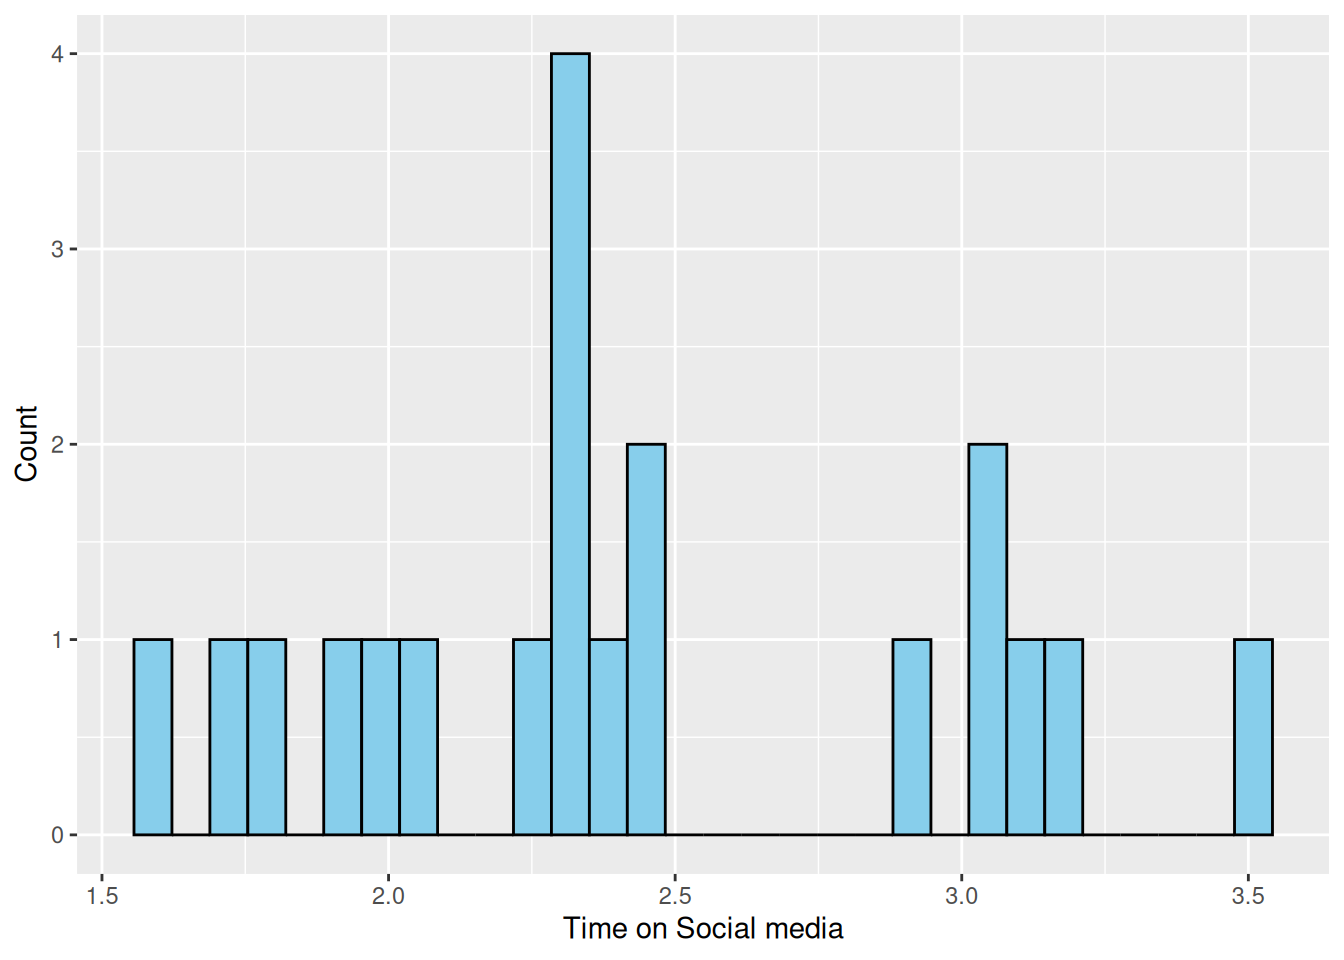
\includegraphics{_main_files/figure-latex/unnamed-chunk-36-1.pdf}

Info: We are using some new aesthetics this week. We use the \texttt{fill} ``skyblue'' and the \texttt{colour} ``black'' to control the interior colour and border of our histogram respectively. You will learn more aesthetics that can be used to create nicer looking plots each week.

Question: What is the shape of the histogram here ? Is it as you expected ?

\section{What does the sampling distribution of the mean look like as we add more samples?}\label{what-does-the-sampling-distribution-of-the-mean-look-like-as-we-add-more-samples}

Now lets see what happens when we add in more samples.

\section{Activity 3 - Increasing the sample size}\label{activity-3---increasing-the-sample-size}

Are you able to use the \texttt{sample()} function, \texttt{data.frame} function to create objects with 100, 250, 350 and 500 samples ? Use the code blocks below to do this.
If you need any help please ask your tutor !

Hint: This is just replicating what we have done above with some new object names.

\begin{Shaded}
\begin{Highlighting}[]
\CommentTok{\#fill in the code below !}

\NormalTok{mean\_sample\_100 }\OtherTok{\textless{}{-}} \FunctionTok{sample}\NormalTok{(global\_social\_media}\SpecialCharTok{$}\NormalTok{mean\_time\_on\_social, }\AttributeTok{size =} \DecValTok{100}\NormalTok{) }\CommentTok{\#create a sampling distribution of the mean with 100 samples}
  
\NormalTok{mean\_sample\_250 }\OtherTok{\textless{}{-}} \FunctionTok{sample}\NormalTok{(global\_social\_media}\SpecialCharTok{$}\NormalTok{mean\_time\_on\_social, }\AttributeTok{size =} \DecValTok{250}\NormalTok{) }\CommentTok{\#create a sampling distribution of the mean with 250 samples}
  
\NormalTok{mean\_sample\_350 }\OtherTok{\textless{}{-}} \FunctionTok{sample}\NormalTok{(global\_social\_media}\SpecialCharTok{$}\NormalTok{mean\_time\_on\_social, }\AttributeTok{size =} \DecValTok{350}\NormalTok{) }\CommentTok{\#create a sampling distribution of the mean with 350 samples}
  
\NormalTok{mean\_sample\_500 }\OtherTok{\textless{}{-}} \FunctionTok{sample}\NormalTok{(global\_social\_media}\SpecialCharTok{$}\NormalTok{mean\_time\_on\_social, }\AttributeTok{size =} \DecValTok{500}\NormalTok{) }\CommentTok{\#create a sampling distribution of the mean with 500 samples}
\end{Highlighting}
\end{Shaded}

\begin{Shaded}
\begin{Highlighting}[]
\CommentTok{\#fill in the code below ! }
\NormalTok{mean\_sample\_100\_df }\OtherTok{\textless{}{-}} \FunctionTok{data.frame}\NormalTok{(}\AttributeTok{sample\_100 =}\NormalTok{ mean\_sample\_100) }\CommentTok{\#create a dataframe with a column called sample\_100 that takes values from our vector}

\NormalTok{mean\_sample\_250\_df }\OtherTok{\textless{}{-}} \FunctionTok{data.frame}\NormalTok{(}\AttributeTok{sample\_250 =}\NormalTok{ mean\_sample\_250) }\CommentTok{\#create a dataframe with a column called sample\_250 that takes values from our vector}

\NormalTok{mean\_sample\_350\_df }\OtherTok{\textless{}{-}} \FunctionTok{data.frame}\NormalTok{(}\AttributeTok{sample\_350 =}\NormalTok{ mean\_sample\_350) }\CommentTok{\#create a dataframe with a column called sample\_350 that takes values from our vector}

\NormalTok{mean\_sample\_500\_df }\OtherTok{\textless{}{-}} \FunctionTok{data.frame}\NormalTok{(}\AttributeTok{sample\_500 =}\NormalTok{ mean\_sample\_500) }\CommentTok{\#create a dataframe with a column called sample\_500 that takes values from our vector}
\end{Highlighting}
\end{Shaded}

Well done ! This was a hard activity. It you are struggling please ask your tutor for help.

\textbackslash begin\{figure\}

\{\centering \includegraphics[width=0.5\linewidth]{https://github.com/BsoCool/UNSW-PSYC2001/blob/main/All%20images%20for%20computing%20tutorials/What_is_the_sampling_distribution_of_the_mean/Ask%20for%20Help%20!.jpg?raw=true} 

}

\caption{Ask for help !}

\label{fig:unnamed-chunk-37}
\textbackslash end\{figure\}

\section{Activity 4 - Visualising the sampling distribution of the mean with increasing samples}\label{activity-4---visualising-the-sampling-distribution-of-the-mean-with-increasing-samples}

Next we need to visualise all of these new samples. It is important we do this so we can see what happens to our sampling distribution of the mean as we increase the number of mean samples.

We can do this by repeating the code for each histogram and giving it a new fill colour ! Are you able to help with this? (Note there are of course much cleaner ways to do this, if you are interested please see the guide \href{https://www.datacamp.com/f/facets-ggplot-r?utm_source=google&utm_medium=paid_search&utm_campaignid=19589720824&utm_adgroupid=157156376351&utm_device=c&utm_keyword=&utm_matchtype=&utm_network=g&utm_adpostion=&utm_creative=733936254686&utm_targetid=aud-1832882613722:dsa-2218886984060&utm_loc_interest_ms=&utm_loc_physical_ms=9071851&utm_content=ps-other~apac-en~dsa~tofu~tutorial-r-programming&accountid=9624585688&utm_campaign=230119_1-ps-other~dsa~tofu_2-b2c_3-apac_4-prc_5-na_6-na_7-le_8-pdsh-go_9-nb-e_10-na_11-na&gad_source=1&gad_campaignid=19589720824&gbraid=0AAAAADQ9WsHmSJoqa8-5deMNCCGmJAmEp&gclid=CjwKCAjw9anCBhAWEiwAqBJ-c-0oZYPE5pP4Y6ZpYz0WabsrMLtJizQQn90osQAeAOfbaV9oUkleMxoClE4QAvD_BwE}{here}).

\begin{Shaded}
\begin{Highlighting}[]
\NormalTok{mean\_sample\_100\_df }\SpecialCharTok{\%\textgreater{}\%} 
\FunctionTok{ggplot}\NormalTok{(}\FunctionTok{aes}\NormalTok{(}\AttributeTok{x =}\NormalTok{ sample\_100)) }\SpecialCharTok{+}
  \FunctionTok{geom\_histogram}\NormalTok{(}\AttributeTok{fill =} \StringTok{"red"}\NormalTok{, }\AttributeTok{colour =} \StringTok{"black"}\NormalTok{) }\SpecialCharTok{+}
    \FunctionTok{labs}\NormalTok{(}\AttributeTok{x =} \StringTok{"Time on Social media"}\NormalTok{, }\AttributeTok{y =} \StringTok{"Count"}\NormalTok{)}
\end{Highlighting}
\end{Shaded}

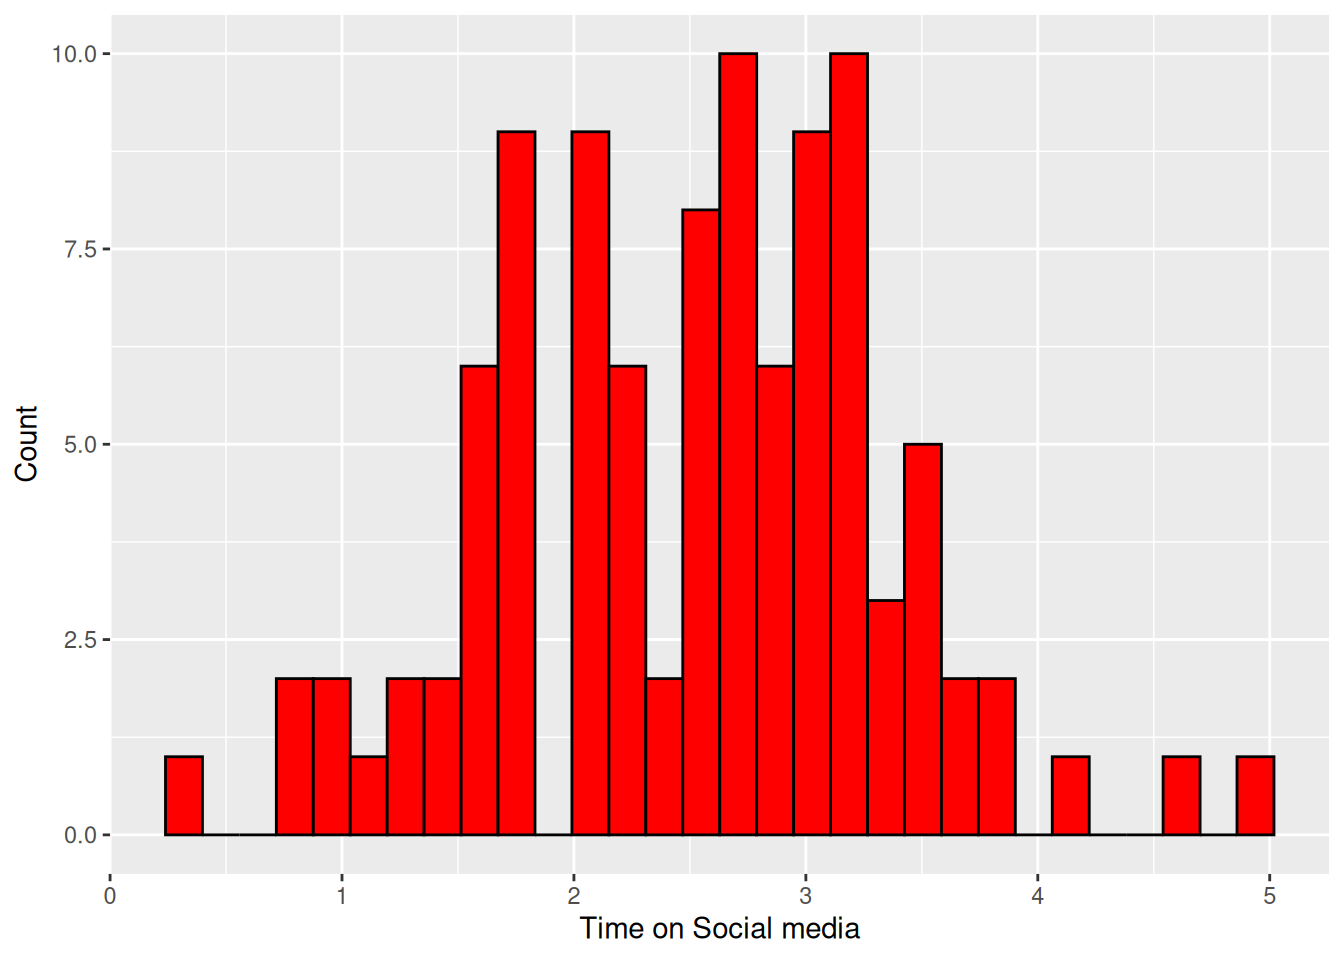
\includegraphics{_main_files/figure-latex/creating histograms for all samples-1.pdf}

\begin{Shaded}
\begin{Highlighting}[]
\NormalTok{mean\_sample\_250\_df }\SpecialCharTok{\%\textgreater{}\%} 
\FunctionTok{ggplot}\NormalTok{(}\FunctionTok{aes}\NormalTok{(}\AttributeTok{x =}\NormalTok{ sample\_250)) }\SpecialCharTok{+}
  \FunctionTok{geom\_histogram}\NormalTok{(}\AttributeTok{fill =} \StringTok{"blue"}\NormalTok{, }\AttributeTok{colour =} \StringTok{"black"}\NormalTok{) }\SpecialCharTok{+}
    \FunctionTok{labs}\NormalTok{(}\AttributeTok{x =} \StringTok{"Time on Social media"}\NormalTok{, }\AttributeTok{y =} \StringTok{"Count"}\NormalTok{)}
\end{Highlighting}
\end{Shaded}

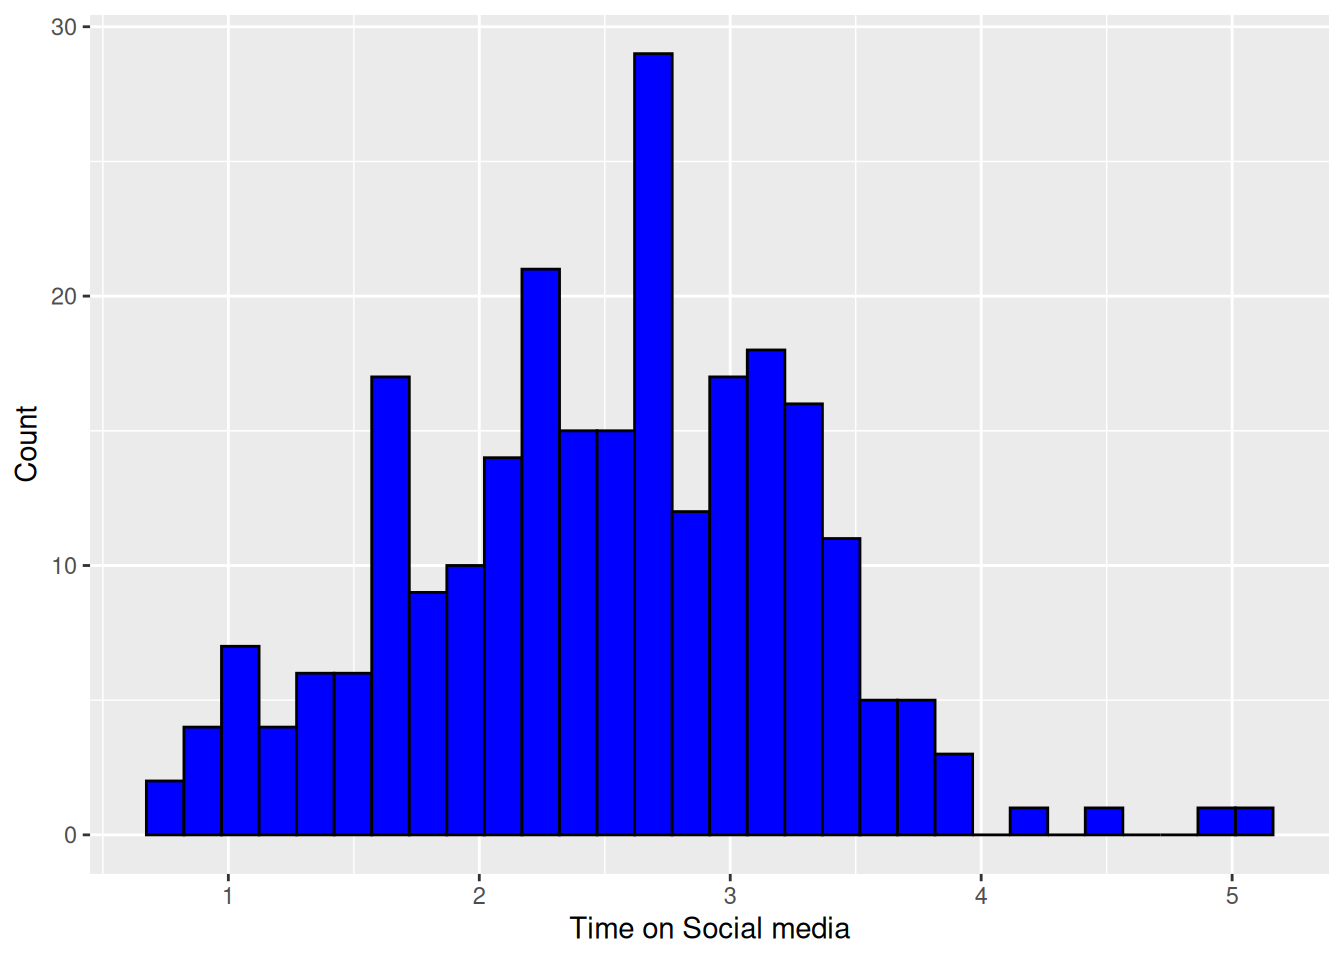
\includegraphics{_main_files/figure-latex/creating histograms for all samples-2.pdf}

\begin{Shaded}
\begin{Highlighting}[]
\NormalTok{mean\_sample\_350\_df }\SpecialCharTok{\%\textgreater{}\%} 
\FunctionTok{ggplot}\NormalTok{(}\FunctionTok{aes}\NormalTok{(}\AttributeTok{x =}\NormalTok{ sample\_350)) }\SpecialCharTok{+}
  \FunctionTok{geom\_histogram}\NormalTok{(}\AttributeTok{fill =} \StringTok{"green"}\NormalTok{, }\AttributeTok{colour =} \StringTok{"black"}\NormalTok{)}\SpecialCharTok{+}
    \FunctionTok{labs}\NormalTok{(}\AttributeTok{x =} \StringTok{"Time on Social media"}\NormalTok{, }\AttributeTok{y =} \StringTok{"Count"}\NormalTok{)}
\end{Highlighting}
\end{Shaded}

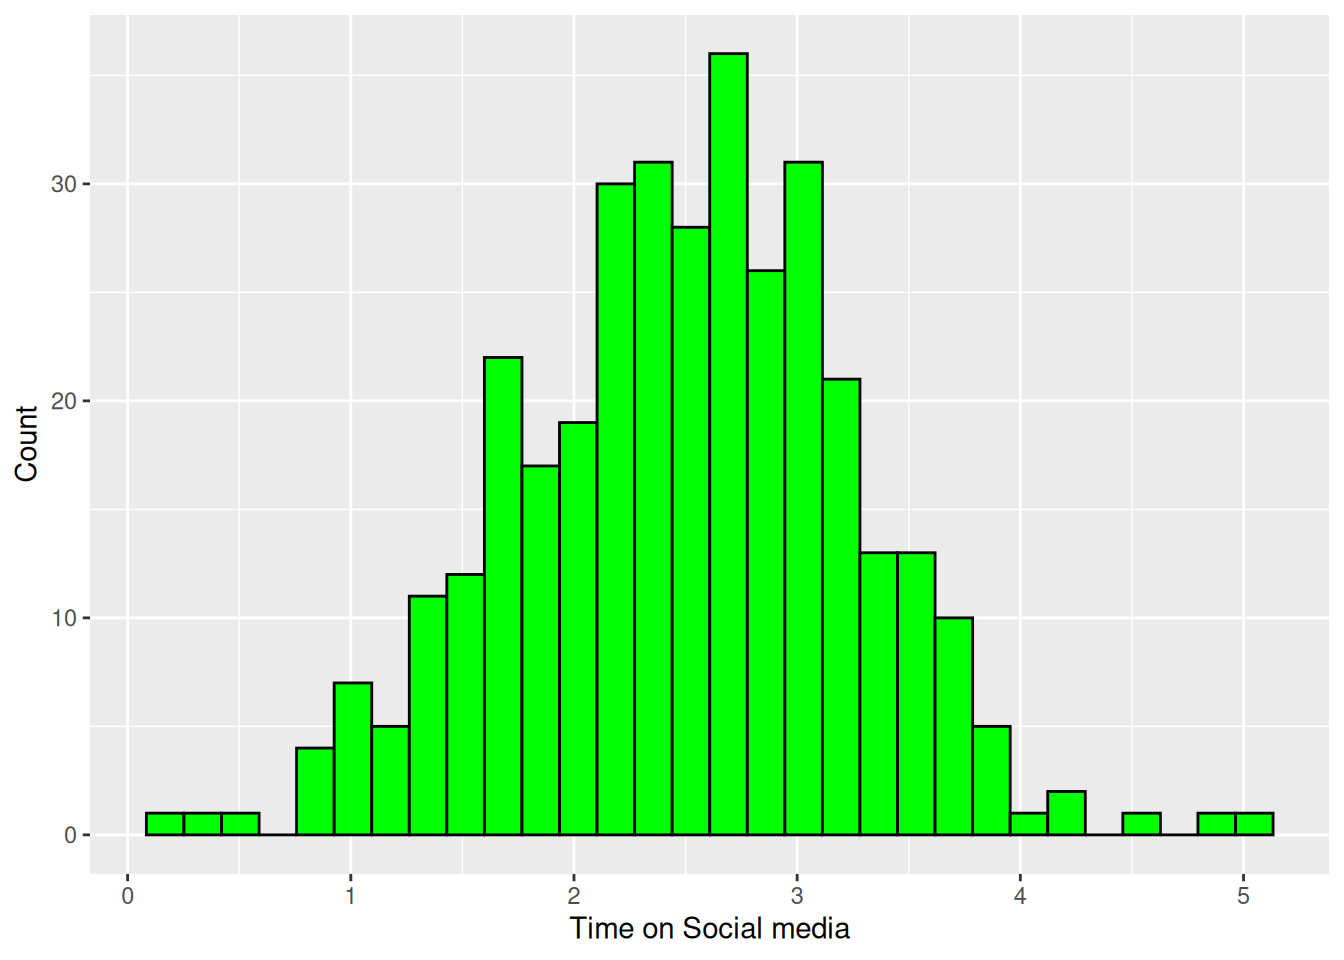
\includegraphics{_main_files/figure-latex/creating histograms for all samples-3.pdf}

\begin{Shaded}
\begin{Highlighting}[]
\NormalTok{mean\_sample\_500\_df }\SpecialCharTok{\%\textgreater{}\%} 
\FunctionTok{ggplot}\NormalTok{(}\FunctionTok{aes}\NormalTok{(}\AttributeTok{x =}\NormalTok{ sample\_500)) }\SpecialCharTok{+}
  \FunctionTok{geom\_histogram}\NormalTok{(}\AttributeTok{fill =} \StringTok{"orange"}\NormalTok{, }\AttributeTok{colour =} \StringTok{"black"}\NormalTok{) }\SpecialCharTok{+}
    \FunctionTok{labs}\NormalTok{(}\AttributeTok{x =} \StringTok{"Time on Social media"}\NormalTok{, }\AttributeTok{y =} \StringTok{"Count"}\NormalTok{)}
\end{Highlighting}
\end{Shaded}

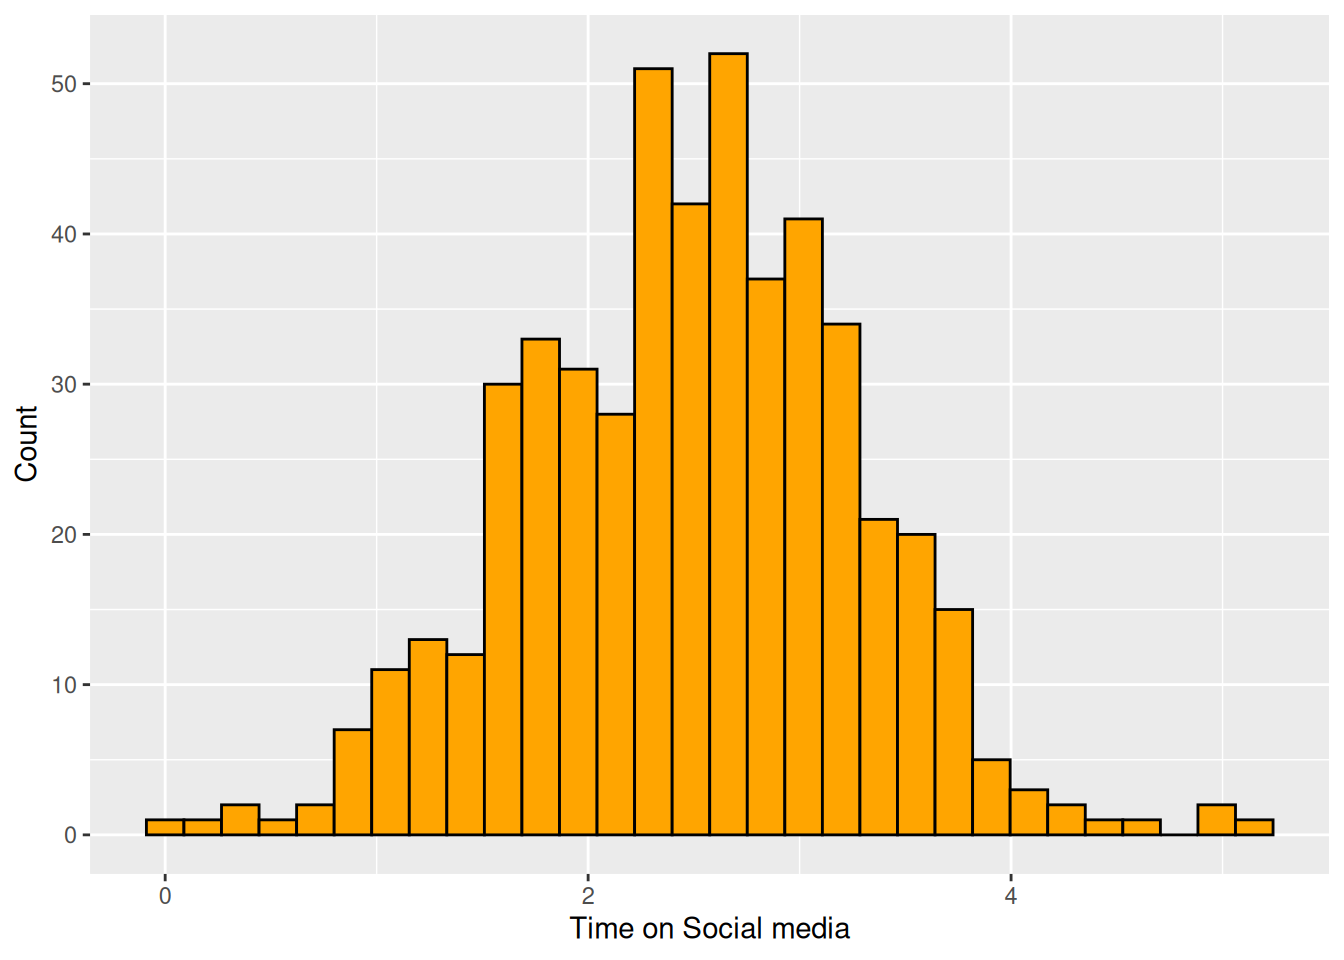
\includegraphics{_main_files/figure-latex/creating histograms for all samples-4.pdf}

Question: How did the histogram change? Is it what you expected? Discuss this with your neighbours and your tutor.

Now imagine that there were infinite universities that ran this experiment, that each collected a group of people's \texttt{time\_on\_social} scores, and each gave us their sample mean value. That is the theoretical sampling distribution of the mean.

The change in the shape of the histogram we have observed here is a critical implication of the central limit theorem - a large number of samples will lead to a approximately normal sampling distribution of the mean regardless of the actual population distribution.

Question: Now thats all well and good but what does this actually mean ? Why do you think this actually matters for the statistics we do ? Discuss this with your neighbour and tutors.

\section{Extension - What happens to a the sampling distribution of the mean for other population distributions ?}\label{extension---what-happens-to-a-the-sampling-distribution-of-the-mean-for-other-population-distributions}

This section is an extension activity if you have already finished the required materials. Please check with your tutor that you have a good grasp of the material before moving onto this section.

\textbackslash begin\{figure\}

\{\centering \includegraphics[width=0.5\linewidth]{https://github.com/BsoCool/UNSW-PSYC2001/blob/main/All%20images%20for%20computing%20tutorials/What_is_the_sampling_distribution_of_the_mean/Extension%20students.gif?raw=true} 

}

\caption{Extension students be like}

\label{fig:unnamed-chunk-38}
\textbackslash end\{figure\}

Now lets get into it. Lets see what happens when we use an exponential population distribution and find its sampling distribution of the mean with a large number of samples.

First, we are going to generate the population distribution. This can be done easily using the function \texttt{rexp()} which is used to generate exponential distributions.

\begin{Shaded}
\begin{Highlighting}[]
\CommentTok{\# Generate an exponential population distribution}
\NormalTok{population }\OtherTok{\textless{}{-}} \FunctionTok{data.frame}\NormalTok{(}\AttributeTok{value =} \FunctionTok{rexp}\NormalTok{(}\DecValTok{100000}\NormalTok{, }\AttributeTok{rate =} \DecValTok{1}\NormalTok{)) }\CommentTok{\#generate an expotential distribution with 100,000 datapoints. }
\end{Highlighting}
\end{Shaded}

Next lets generate a histogram of this population distribution and confirm that it looks like an exponential distribution.

\begin{Shaded}
\begin{Highlighting}[]
\CommentTok{\# Plot population distribution}
\FunctionTok{ggplot}\NormalTok{(population, }\FunctionTok{aes}\NormalTok{(}\AttributeTok{x =}\NormalTok{ value)) }\SpecialCharTok{+}
  \FunctionTok{geom\_histogram}\NormalTok{( }\AttributeTok{bins =} \DecValTok{100}\NormalTok{, }\AttributeTok{fill =} \StringTok{"skyblue"}\NormalTok{, }\AttributeTok{color =} \StringTok{"black"}\NormalTok{) }\SpecialCharTok{+}
  \FunctionTok{labs}\NormalTok{(}
       \AttributeTok{x =} \StringTok{"Value"}\NormalTok{,}
       \AttributeTok{y =} \StringTok{"Frequency"}\NormalTok{) }\SpecialCharTok{+}
  \FunctionTok{theme\_classic}\NormalTok{() }\CommentTok{\#themes can be provided to ggplot which give it a bunch of aesthetics to change. One of these is theme\_classic}
\end{Highlighting}
\end{Shaded}

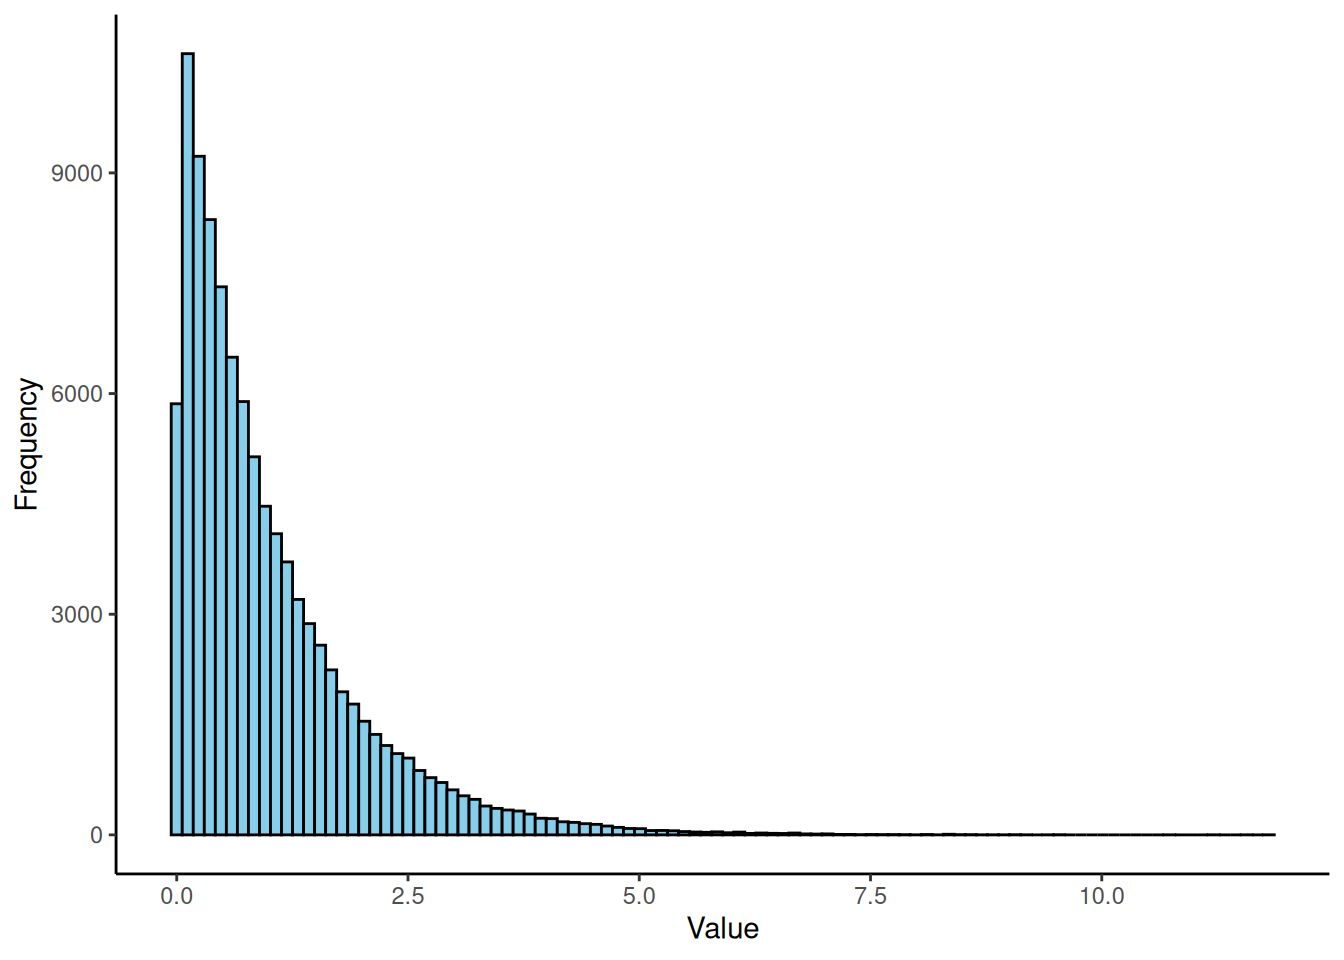
\includegraphics{_main_files/figure-latex/unnamed-chunk-40-1.pdf}

Question: Do you think this looks like an exponential distribution ? What should an exponential distribution look like ? Ask your tutor if you are not sure !

Now we can take samples from this population. We use a new function here could \texttt{replicate()} which basically repeats the process inside the \texttt{\{\}} brackets a specified number of times. Inside the \texttt{\{\}} brackets is what we are actually doing population distribution. First we are taking a sample using the \texttt{sample()} function, then we are taking the mean of that sample using the \texttt{mean()} function. This will generate a similar set of data to \texttt{PSYC2001\_global-time-on-social-data.csv}. That is, means of a bunch of samples from the population (i.e the sampling distirbution of the mean)

\begin{Shaded}
\begin{Highlighting}[]
\CommentTok{\# Lets take 500 samples from this population of size 50 per sample and calculate the mean. }
\NormalTok{sample\_means }\OtherTok{\textless{}{-}} \FunctionTok{replicate}\NormalTok{(}\DecValTok{500}\NormalTok{, \{ }\CommentTok{\#replicate the process 500 times}
\NormalTok{  sample\_values }\OtherTok{\textless{}{-}} \FunctionTok{sample}\NormalTok{(population}\SpecialCharTok{$}\NormalTok{value, }\AttributeTok{size =} \DecValTok{50}\NormalTok{, }\AttributeTok{replace =} \ConstantTok{TRUE}\NormalTok{) }\CommentTok{\# sample 50 values from the population mean}
  \FunctionTok{mean}\NormalTok{(sample\_values) }\CommentTok{\#take the mean of those 50 sampled values}
\NormalTok{\})}
\end{Highlighting}
\end{Shaded}

So what we have generated is a sampling distribution of the mean with 500 samples. Lets first convert that into a dataframe so that we can use \texttt{ggplot} to visualise this data.

\begin{Shaded}
\begin{Highlighting}[]
\CommentTok{\# Put results in a dataframe for plotting}
\NormalTok{sampling\_df }\OtherTok{\textless{}{-}} \FunctionTok{data.frame}\NormalTok{(}\AttributeTok{sample\_mean =}\NormalTok{ sample\_means) }\CommentTok{\#convert the result into a dataframe}

\CommentTok{\#plot the results}
\NormalTok{sampling\_df }\SpecialCharTok{\%\textgreater{}\%} 
\FunctionTok{ggplot}\NormalTok{(}\FunctionTok{aes}\NormalTok{(}\AttributeTok{x =}\NormalTok{ sample\_mean)) }\SpecialCharTok{+}
  \FunctionTok{geom\_histogram}\NormalTok{(}\AttributeTok{fill =} \StringTok{"skyblue"}\NormalTok{, }\AttributeTok{color =} \StringTok{"black"}\NormalTok{) }\SpecialCharTok{+}
  \FunctionTok{labs}\NormalTok{(}\AttributeTok{x =} \StringTok{"Sample Mean"}\NormalTok{, }\AttributeTok{y =} \StringTok{"Frequency"}\NormalTok{) }\SpecialCharTok{+}
  \FunctionTok{theme\_classic}\NormalTok{()}
\end{Highlighting}
\end{Shaded}

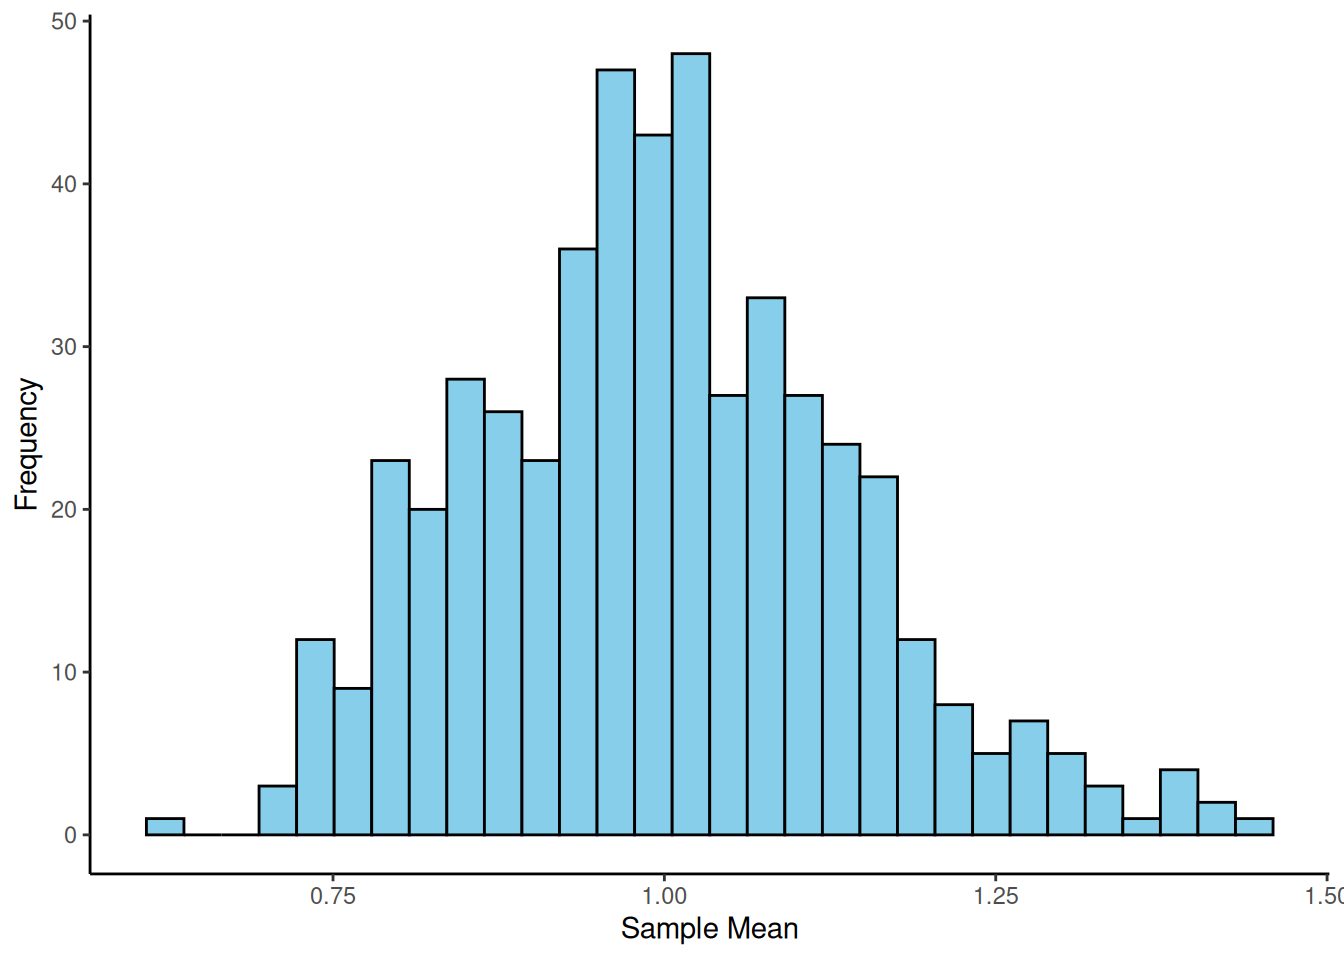
\includegraphics{_main_files/figure-latex/unnamed-chunk-42-1.pdf}

Question: What is the shape of this distribution ? is it different to the population distribution from above ? What are the implications of this ?

\section{You are Free!}\label{you-are-free-2}

Well done you have completed another computing tutorial. This one has been very difficult and you have done a terrific job. See you all next week for more computing fun !

\textbackslash begin\{figure\}

\{\centering \includegraphics[width=0.75\linewidth]{https://github.com/BsoCool/UNSW-PSYC2001/blob/main/All%20images%20for%20computing%20tutorials/What_is_the_sampling_distribution_of_the_mean/Crab%20celebration.gif?raw=true} 

}

\caption{Celebrating finishing this tutorial !}

\label{fig:unnamed-chunk-43}
\textbackslash end\{figure\}

\chapter{Testing our first hypothesis}\label{testing-our-first-hypothesis}

Today we are going to ask our first question and seek an answer from the data. We will get the data into shape so that it is in the right format for visualizing and analysing. Then we will run the analysis and learn the answer to our question. Welcome. You are now a psychologist :)

\section{Checking installation and loading packages}\label{checking-installation-and-loading-packages-2}

As usual we first always check and load in our required packages.

\begin{Shaded}
\begin{Highlighting}[]
\CommentTok{\# Check if packages are installed, if not install.}
\ControlFlowTok{if}\NormalTok{(}\SpecialCharTok{!}\FunctionTok{require}\NormalTok{(here)) }\FunctionTok{install.packages}\NormalTok{(}\StringTok{\textquotesingle{}here\textquotesingle{}}\NormalTok{) }\CommentTok{\#checks if a package is installed and installs it if required.}
\ControlFlowTok{if}\NormalTok{(}\SpecialCharTok{!}\FunctionTok{require}\NormalTok{(tidyverse)) }\FunctionTok{install.packages}\NormalTok{(}\StringTok{\textquotesingle{}tidyverse\textquotesingle{}}\NormalTok{)}
\ControlFlowTok{if}\NormalTok{(}\SpecialCharTok{!}\FunctionTok{require}\NormalTok{(ggplot2)) }\FunctionTok{install.packages}\NormalTok{(}\StringTok{\textquotesingle{}ggplot2\textquotesingle{}}\NormalTok{)}

\FunctionTok{library}\NormalTok{(here) }\CommentTok{\#loads in the specified package}
\FunctionTok{library}\NormalTok{(tidyverse)}
\FunctionTok{library}\NormalTok{(ggplot2)}
\end{Highlighting}
\end{Shaded}

\section{Developing our hypotheses}\label{developing-our-hypotheses}

Today we are going to address one of the key questions of the study about social media use -- how does mood affect active social media use? Active social media use involves interacting with content (i.e.~liking posts) rather than just observing posts.

There is some evidence to suggest that passive social media use is associated with lower mood in adolescents, whereas active social media use is related to positive mood \href{https://pmc.ncbi.nlm.nih.gov/articles/PMC7366938/}{Dienlin \& Johannes, 2020}. However, a lot of the existing evidence comes from self-report, rather than measuring social media behaviour directly.

To address this question, the researchers used the participants metadata to count how frequently they liked posts. By cross-referencing this with the mood diary kept by each participant, they were able to calculate the average number of likes per 10 minutes of use when participants were in a good mood, and when they were in a bad mood.

It should be clear by now that we will be addressing this question using the \texttt{good\_mood\_likes} and \texttt{bad\_mood\_likes} varaibles. Remember, these variables stand for the following:

\begin{itemize}
\tightlist
\item
  \texttt{good\_mood\_likes} -- average number of likes made over 10 min during a good mood (from platform + diary)
\item
  \texttt{bad\_mood\_likes} -- as above, but during bad mood
\end{itemize}

\section{Activity 1 - Defining our hypotheses}\label{activity-1---defining-our-hypotheses}

Based on the information above, discuss and formulate hypotheses around the following:

\begin{enumerate}
\def\labelenumi{\arabic{enumi}.}
\tightlist
\item
  Should there be a difference in the number of likes between the mood conditions
\item
  What direction do you think this difference could be? Can you formulate an experimental hypothesis each way -- i.e.~good mood likes \textgreater{} bad mood likes, and vice versa?
\item
  What is the null hypothesis?
\end{enumerate}

Question: Discuss this with your neighbour and your tutor. Make sure you have clearly defined your hypotheses before moving forward.

\section{Visualising our data}\label{visualising-our-data}

First we want to load in the dataset \texttt{PSYC2001\_social-media-data-cleaned.csv} dataset. To do this we use the same \texttt{read.csv()} function combined with \texttt{here()}. Do you remember how to do this ?

\begin{Shaded}
\begin{Highlighting}[]
\NormalTok{social\_media }\OtherTok{\textless{}{-}} \FunctionTok{read.csv}\NormalTok{(}\AttributeTok{file =} \FunctionTok{here}\NormalTok{(}\StringTok{"Data"}\NormalTok{,}\StringTok{"PSYC2001\_social{-}media{-}data{-}cleaned.csv"}\NormalTok{)) }\CommentTok{\#reads in CSV files}
\end{Highlighting}
\end{Shaded}

Before we conduct any kind of statistical test it is a good idea to see how it looks. This will give us an understanding about the underlying data that is driving the results of our statistical test.

Warning: It is generally \textbf{bad practice} to go straight from the raw data to the results of a statistical test without first visualising the data.

\textbackslash begin\{figure\}

\{\centering \includegraphics[width=0.5\linewidth]{https://github.com/BsoCool/UNSW-PSYC2001/blob/main/All%20images%20for%20computing%20tutorials/Testing_our_first_hypothesis/Statistics%20professors%20reaction.gif?raw=true} 

}

\caption{Professors reaction when you don't visualise data}

\label{fig:unnamed-chunk-46}
\textbackslash end\{figure\}

\section{Density plot of the distribution}\label{density-plot-of-the-distribution}

We can look at the distribution of the data using a density plot. A density plot is a smoothed version of a histogram which allows us to understand what the full distribution might look like if we had all the data in the world. More information on that \href{https://www.data-to-viz.com/graph/density.html}{is here} if you are interested !

In order to make this easy to plot we first have to wrangle our data a bit. What we want to do here is convert our data from a wide-format (which is more digestible for us mere humans) into a long format (which programs like R generally like more!). More on that \href{https://www.statology.org/long-vs-wide-data/}{here}.

First we use the \texttt{select()} function which allows us to easily choose which columns we do (or don't) want to keep in our dataframe. Second we use the \texttt{pivot\_longer()} function which allows us to combine different columns together. Both of these functions come from the \texttt{tidyverse} package. In the code below we take the columns ending with ``likes'' and put their values (i.e the number of likes) into the column ``likes'' and their column names names (i.e good or bad mood) into the column ``mood''.

\begin{Shaded}
\begin{Highlighting}[]
\NormalTok{social\_media\_likes }\OtherTok{\textless{}{-}}\NormalTok{ social\_media }\SpecialCharTok{\%\textgreater{}\%} 
  \FunctionTok{select}\NormalTok{(}\StringTok{"id"}\NormalTok{,}\StringTok{"good\_mood\_likes"}\NormalTok{,}\StringTok{"bad\_mood\_likes"}\NormalTok{) }\SpecialCharTok{\%\textgreater{}\%} \CommentTok{\# choose which columns we want keep in our dataframe}
  \FunctionTok{pivot\_longer}\NormalTok{(}\AttributeTok{cols =} \FunctionTok{ends\_with}\NormalTok{(}\StringTok{"likes"}\NormalTok{), }\AttributeTok{names\_to =} \StringTok{"mood"}\NormalTok{, }\AttributeTok{values\_to =} \StringTok{"likes"}\NormalTok{) }\CommentTok{\#take columns ending with "likes" and move the column names into "mood" and column values into "likes"}
\end{Highlighting}
\end{Shaded}

Let's make sure that this data still looks okay by using the \texttt{head()} function.

\begin{Shaded}
\begin{Highlighting}[]
\FunctionTok{head}\NormalTok{(social\_media\_likes)}
\end{Highlighting}
\end{Shaded}

\begin{verbatim}
## # A tibble: 6 x 3
##   id    mood            likes
##   <chr> <chr>           <dbl>
## 1 S1    good_mood_likes  22.8
## 2 S1    bad_mood_likes   46.5
## 3 S2    good_mood_likes  46  
## 4 S2    bad_mood_likes   48.3
## 5 S3    good_mood_likes  50.8
## 6 S3    bad_mood_likes   46.1
\end{verbatim}

Now, we can get a density plot in R by using the \texttt{geom\_density} function inside \texttt{ggplot()}.

\begin{Shaded}
\begin{Highlighting}[]
\NormalTok{social\_media\_likes }\SpecialCharTok{\%\textgreater{}\%} 
\FunctionTok{ggplot}\NormalTok{(}\FunctionTok{aes}\NormalTok{(}\AttributeTok{x =}\NormalTok{ likes, }\AttributeTok{colour =}\NormalTok{ mood)) }\SpecialCharTok{+}
  \FunctionTok{geom\_density}\NormalTok{(}\AttributeTok{linewidth =} \DecValTok{2}\NormalTok{) }\SpecialCharTok{+}
    \FunctionTok{labs}\NormalTok{(}\AttributeTok{x =} \StringTok{"Number of likes"}\NormalTok{, }\AttributeTok{y =} \StringTok{"Density"}\NormalTok{) }\SpecialCharTok{+}
  \FunctionTok{theme\_classic}\NormalTok{() }\CommentTok{\#themes can be provided to ggplot which give it a bunch of aesthetics to change. One of these is theme\_classic}
\end{Highlighting}
\end{Shaded}

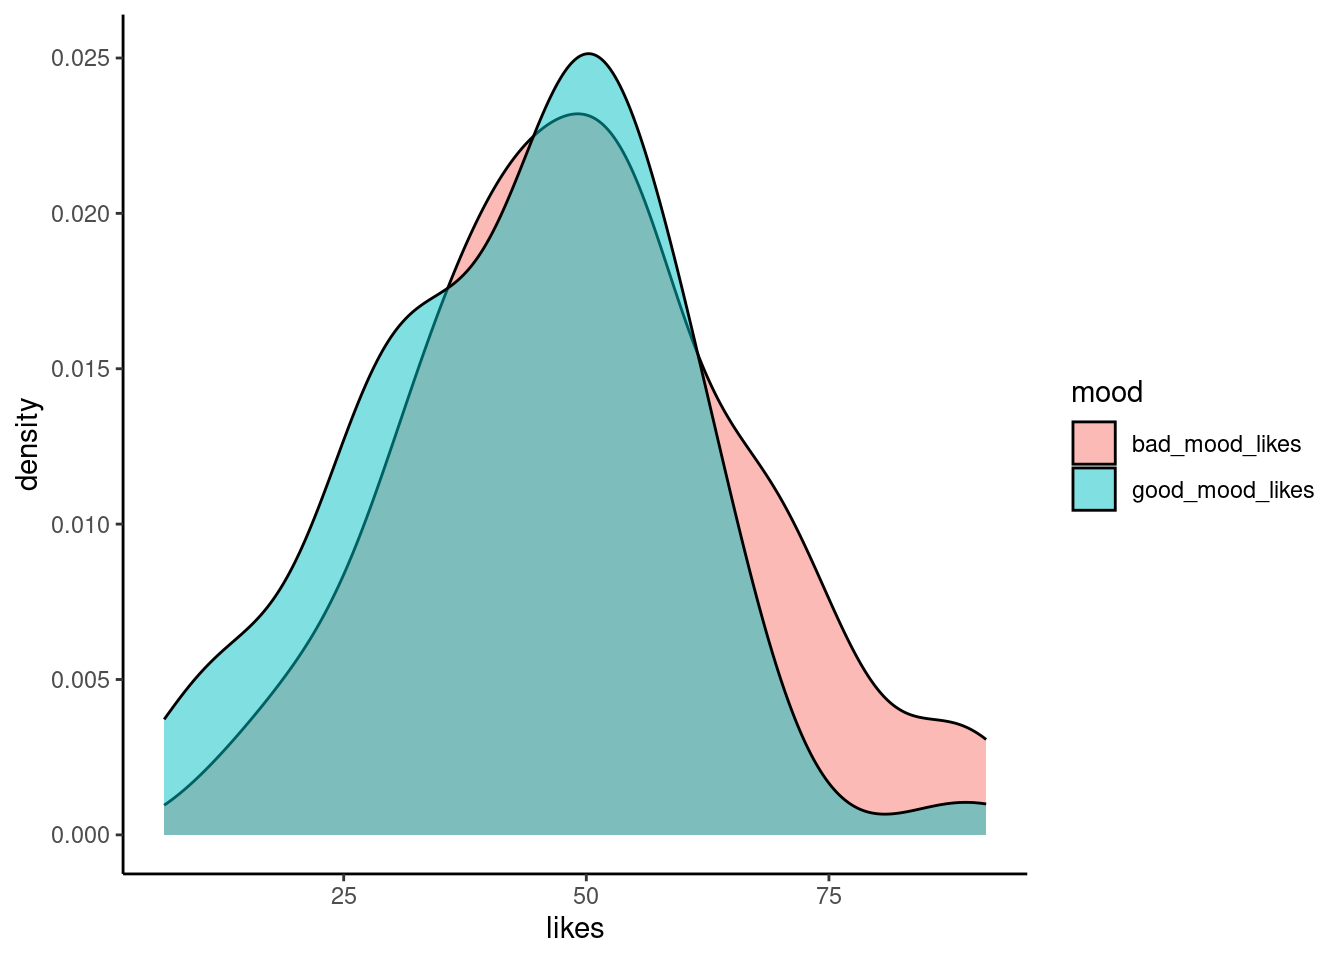
\includegraphics{_main_files/figure-latex/Create a density plot-1.pdf}

Info: We are using a new function here called \texttt{theme\_classic()}. This makes the graph look at a bit nicer. There are a bunch of other available themes \href{https://ggplot2.tidyverse.org/reference/ggtheme.html}{here}. We also have a new argument \texttt{colour} inside the \texttt{aes()} function which tells \texttt{ggplot()} to use different line colours depending on the participants mood (i.e good or bad mood).

\section{Activity 2 - Choosing a new theme}\label{activity-2---choosing-a-new-theme}

Lets have a go at replicating the previous graph but using a new theme. You can pick whichever theme you think looks the best. Notice that changing the theme will only change non-data related aesthetic features of the graph.

\begin{Shaded}
\begin{Highlighting}[]
\NormalTok{social\_media\_likes }\SpecialCharTok{\%\textgreater{}\%} 
\FunctionTok{ggplot}\NormalTok{(}\FunctionTok{aes}\NormalTok{(}\AttributeTok{x =}\NormalTok{ likes, }\AttributeTok{colour =}\NormalTok{ mood)) }\SpecialCharTok{+}
  \FunctionTok{geom\_density}\NormalTok{(}\AttributeTok{linewidth =} \DecValTok{2}\NormalTok{) }\SpecialCharTok{+}
    \FunctionTok{labs}\NormalTok{(}\AttributeTok{x =} \StringTok{"Number of likes"}\NormalTok{, }\AttributeTok{y =} \StringTok{"Density"}\NormalTok{) }\SpecialCharTok{+}
  \FunctionTok{theme\_bw}\NormalTok{() }\CommentTok{\#themes can be provided to ggplot which give it a bunch of aesthetics to change. One of these is theme\_classic}
\end{Highlighting}
\end{Shaded}

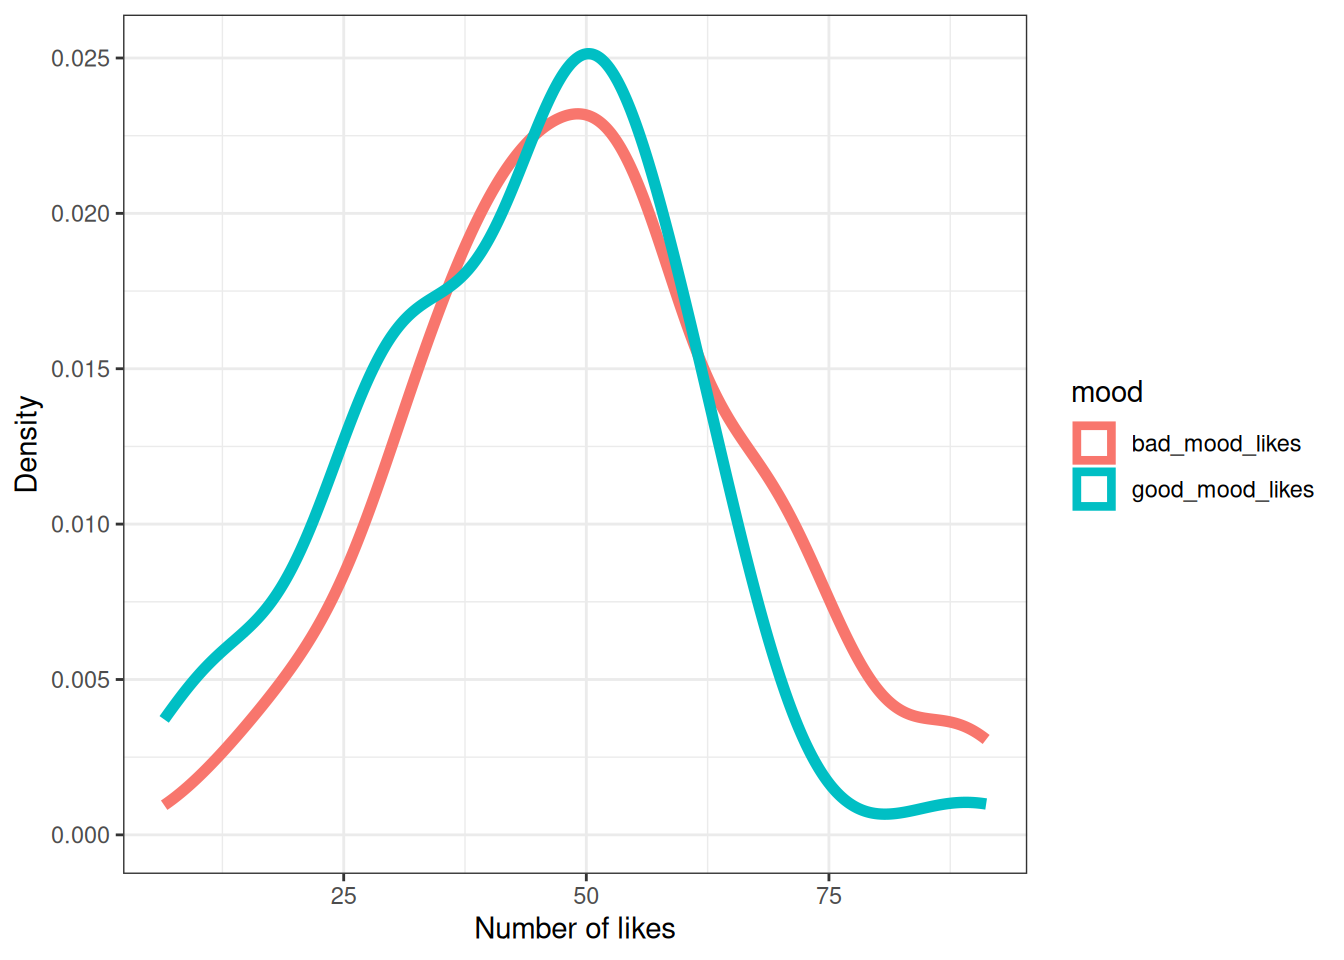
\includegraphics{_main_files/figure-latex/Activity 2 - Changing ggplot themes-1.pdf}

\section{Descriptive statistics}\label{descriptive-statistics}

Before we can move onto conducting t-tests it is always a good idea to generate our descriptive statistics. For the data we are looking at \textbf{the most relevant descriptive statistics are the mean and standard deviation}. This is because we want to conduct a t-test to compare the average likes in different moods. We can easily get this information in R by using the \texttt{summarise()} function together with the \texttt{group\_by()} function. The \texttt{group\_by()} splits the data into different groups and the \texttt{summarise()} function calculates a statistic (i.e the mean and standard deviation). Both of these packages come from the \texttt{tidyverse} package.

\begin{Shaded}
\begin{Highlighting}[]
\NormalTok{social\_media\_descriptives }\OtherTok{\textless{}{-}}\NormalTok{ social\_media\_likes }\SpecialCharTok{\%\textgreater{}\%} 
  \FunctionTok{group\_by}\NormalTok{(mood) }\SpecialCharTok{\%\textgreater{}\%} \CommentTok{\#split the data by mood}
  \FunctionTok{summarise}\NormalTok{(}\AttributeTok{mean\_likes =} \FunctionTok{mean}\NormalTok{(likes),}
            \AttributeTok{sd\_likes =} \FunctionTok{sd}\NormalTok{(likes)) }\CommentTok{\#calculate the mean number of likes}

\FunctionTok{head}\NormalTok{(social\_media\_descriptives)}
\end{Highlighting}
\end{Shaded}

\begin{verbatim}
## # A tibble: 2 x 3
##   mood            mean_likes sd_likes
##   <chr>                <dbl>    <dbl>
## 1 bad_mood_likes        49.8     17.2
## 2 good_mood_likes       43.0     16.1
\end{verbatim}

Question: What are the mean number of likes in each different mood ? What is the standard deviation ?

\section{Activity 3 - Calculating the median number of likes}\label{activity-3---calculating-the-median-number-of-likes}

Great ! We have the mean number of likes when subjects are in a good and bad mood. Please see if you are able to use these functions to instead calculate the median number of likes under different mood conditions.

Hint: The \texttt{median()} function is used to calculate medians !

\begin{Shaded}
\begin{Highlighting}[]
\NormalTok{social\_media\_median }\OtherTok{\textless{}{-}}\NormalTok{ social\_media\_likes }\SpecialCharTok{\%\textgreater{}\%} 
  \FunctionTok{group\_by}\NormalTok{(mood) }\SpecialCharTok{\%\textgreater{}\%} \CommentTok{\#split the data by mood}
  \FunctionTok{summarise}\NormalTok{(}\AttributeTok{median\_likes =} \FunctionTok{median}\NormalTok{(likes)) }\CommentTok{\#calculate the mean number of likes}

\FunctionTok{head}\NormalTok{(social\_media\_median)}
\end{Highlighting}
\end{Shaded}

\begin{verbatim}
## # A tibble: 2 x 2
##   mood            median_likes
##   <chr>                  <dbl>
## 1 bad_mood_likes          49.3
## 2 good_mood_likes         45.9
\end{verbatim}

\section{Testing hypotheses manually}\label{testing-hypotheses-manually}

Now that we have had a look at the structure and descriptives statistics of our data we can have a go at using a t-test to compare the number of likes participants made in a good and bad mood. We could of course do this manually, by hand (as we have in the statistics tutorials). We have shown this below using the first 10 values for good and bad mood likes.

\textbackslash begin\{figure\}

\{\centering \includegraphics[width=0.75\linewidth]{https://github.com/BsoCool/UNSW-PSYC2001/blob/main/All%20images%20for%20computing%20tutorials/Testing_our_first_hypothesis/Manual%20t-test%20table.JPG?raw=true} 

}

\caption{t-test table}

\label{fig:unnamed-chunk-49}
\textbackslash end\{figure\}

Thankfully, we have long since past the stone (pen) age so it is no longer necessary to do this by hand. We can get computers to do this for us!

\begin{figure}

{\centering \includegraphics[width=0.5\linewidth]{https://github.com/BsoCool/UNSW-PSYC2001/blob/main/All%20images%20for%20computing%20tutorials/Testing_our_first_hypothesis/Space%20odyssey.gif?raw=true
} 

}

\caption{Handwritten statistiscs be like}\label{fig:unnamed-chunk-50}
\end{figure}

\section{Testing hypothesis using a two-sample t-test}\label{testing-hypothesis-using-a-two-sample-t-test}

We can very easily calculate a t-test in R using the \texttt{t.test()} function which comes as part of \texttt{baseR}. Please first have a look at this function using the \texttt{?} syntax to understand its arguments. We recommend using the console from now on to do this rather than creating a codeblock.

\textbackslash begin\{figure\}

\{\centering \includegraphics[width=1\linewidth]{https://github.com/BsoCool/UNSW-PSYC2001/blob/main/All%20images%20for%20computing%20tutorials/Testing_our_first_hypothesis/Navigating%20to%20the%20Console.gif?raw=true} 

}

\caption{Finding the Console}

\label{fig:unnamed-chunk-51}
\textbackslash end\{figure\}

We can see that \texttt{t.test()} takes different arguments which are important for the way it handles the data. What values you provide to these arguments is dependent on what kind of test you want to conduct. One of the most important arguments to fill in is the \texttt{paired} argument. This determines whether you are conducting an independent or paired samples t-test. Here, we have collected the number of likes for the same subject in different moods. This means this data comes from a repeated-measures design, and so a paired t-test is most appropriate. We also need to provide \texttt{t.test()} with a formula telling it what to do with our data. The left hand side is the numerical variable and the right hand side is a grouping variable.

\begin{Shaded}
\begin{Highlighting}[]
\FunctionTok{t.test}\NormalTok{(}\AttributeTok{formula =}\NormalTok{ likes }\SpecialCharTok{\textasciitilde{}}\NormalTok{ mood, }\AttributeTok{data =}\NormalTok{ social\_media\_likes, }\AttributeTok{paired =} \ConstantTok{TRUE}\NormalTok{)  }\CommentTok{\#compute a t{-}test. Likes \textasciitilde{} mood indicates that likes is the numerical variable and mood is a grouping variables. Paired indicates whether to conduct a paired or independent t{-}test.}
\end{Highlighting}
\end{Shaded}

\begin{verbatim}
## 
##  Paired t-test
## 
## data:  likes by mood
## t = 3.336, df = 59, p-value = 0.001474
## alternative hypothesis: true mean difference is not equal to 0
## 95 percent confidence interval:
##   2.721958 10.881375
## sample estimates:
## mean difference 
##        6.801667
\end{verbatim}

Question: Discuss the output of this paired t-test with your neighbour and tutors. What does it tell us ?

\section{Activity 4 - One-sample t-tests}\label{activity-4---one-sample-t-tests}

Now that we have the output of a paired t-test we can compare it to a one sample t-test. The results of both of these tests should be identical (this has been covered in the lectures). For those that haven't watched the lectures, this is because a paired t-test is basically a one-sample t-test of matched difference scores (\href{https://statisticsbyjim.com/hypothesis-testing/t-tests-1-sample-2-sample-paired-t-tests/}{more on that here})

Are you able to conduct a one-sample t-test using R ?

First you will need to use the \texttt{mutate()} function on the original \texttt{social\_media} dataframe to create a difference column.

\begin{Shaded}
\begin{Highlighting}[]
\NormalTok{social\_media\_diff }\OtherTok{\textless{}{-}}\NormalTok{ social\_media }\SpecialCharTok{\%\textgreater{}\%} 
  \FunctionTok{mutate}\NormalTok{(}\AttributeTok{likes\_diff =}\NormalTok{ good\_mood\_likes }\SpecialCharTok{{-}}\NormalTok{ bad\_mood\_likes) }\CommentTok{\#first try to create a new column which is the difference between mood likes}

\FunctionTok{head}\NormalTok{(social\_media\_diff)}
\end{Highlighting}
\end{Shaded}

\begin{verbatim}
##   X id  age time_on_social urban good_mood_likes bad_mood_likes followers
## 1 1 S1 15.2           3.06     1            22.8           46.5     173.3
## 2 2 S2 16.0           2.18     1            46.0           48.3     144.3
## 3 3 S3 16.8           1.92     1            50.8           46.1      76.5
## 4 4 S4 15.6           2.61     1            29.9           29.2     171.7
## 5 5 S5 17.1           3.24     1            37.1           52.4     109.5
## 6 6 S6 15.7           2.44     1            26.9           20.2     157.5
##   polit_informed polit_campaign polit_activism likes_diff
## 1            2.3            3.2            3.6      -23.7
## 2            1.6            2.2            2.6       -2.3
## 3            1.9            2.7            3.0        4.7
## 4            1.6            2.3            2.6        0.7
## 5            2.0            2.9            3.3      -15.3
## 6            2.4            3.4            3.9        6.7
\end{verbatim}

Once we have correctly calculated our difference score we can use the \texttt{t.test()} function to get our results.

\begin{Shaded}
\begin{Highlighting}[]
\FunctionTok{t.test}\NormalTok{(}\AttributeTok{formula =}\NormalTok{ likes\_diff}\SpecialCharTok{\textasciitilde{}}\DecValTok{1}\NormalTok{, }\AttributeTok{data =}\NormalTok{ social\_media\_diff) }\CommentTok{\#the formula likes\_diff\textasciitilde{}1 indicates that there is no grouping variables (i.e just compare to 0!)}
\end{Highlighting}
\end{Shaded}

\begin{verbatim}
## 
##  One Sample t-test
## 
## data:  likes_diff
## t = -3.336, df = 59, p-value = 0.001474
## alternative hypothesis: true mean is not equal to 0
## 95 percent confidence interval:
##  -10.881375  -2.721958
## sample estimates:
## mean of x 
## -6.801667
\end{verbatim}

Info: The right hand side of the formula `likes\_diff\textasciitilde{}\textbf{1}' indicates that there is no grouping variable.

Question: Compare the output of the one-sample t-test and the paired t-test. Are they the same ?

\section{Writing up results and conclusions}\label{writing-up-results-and-conclusions}

Let's have a go at writing up the results of the paired samples t-test we have conducted in APA format. While it is not necessarily critical to use APA formatting outside of these psychology courses, it is important to follow some existing format so that readers can easily interpret your results and conclusions about important data.

Results: A paired samples t-test indicated that the number of likes was greater when participants were in a bad mood (M = 49.8 , SD = 17.2) than in a good mood (M = 43.0 , SD = 16.1) and this difference was statistically significant (t(59) = 3.336, p = 0.001).

What can we conclude from this? Please have a go at writing this up.

Conclusions: Your conclusion will go here !

\section{Plotting our results}\label{plotting-our-results}

Now that we have conducted our statistical test we need to present the results in the simplest way possible. One way to do this is by using the average number of likes when participants are in a good and bad mood and plotting it using a column graph.

\section{Activity 5 - Plotting the mean number of likes}\label{activity-5---plotting-the-mean-number-of-likes}

Are you able to plot the mean number of likes as a column graph ?

Hint: This will be very similar to the code used to plot the density graph but instead using \texttt{geom\_col()}.

\begin{Shaded}
\begin{Highlighting}[]
\NormalTok{social\_media\_descriptives }\SpecialCharTok{\%\textgreater{}\%}   \CommentTok{\#write code that produces a column graph of likes with a different colour for each mood}
\FunctionTok{ggplot}\NormalTok{(}\FunctionTok{aes}\NormalTok{(}\AttributeTok{y =}\NormalTok{ mean\_likes, }\AttributeTok{x =}\NormalTok{ mood, }\AttributeTok{fill =}\NormalTok{ mood)) }\SpecialCharTok{+}
  \FunctionTok{geom\_col}\NormalTok{(}\AttributeTok{linewidth =} \DecValTok{2}\NormalTok{) }\SpecialCharTok{+}
    \FunctionTok{labs}\NormalTok{(}\AttributeTok{y =} \StringTok{"Number of likes"}\NormalTok{, }\AttributeTok{x =} \StringTok{"Mood"}\NormalTok{)}\SpecialCharTok{+}
  \FunctionTok{theme\_classic}\NormalTok{()}
\end{Highlighting}
\end{Shaded}

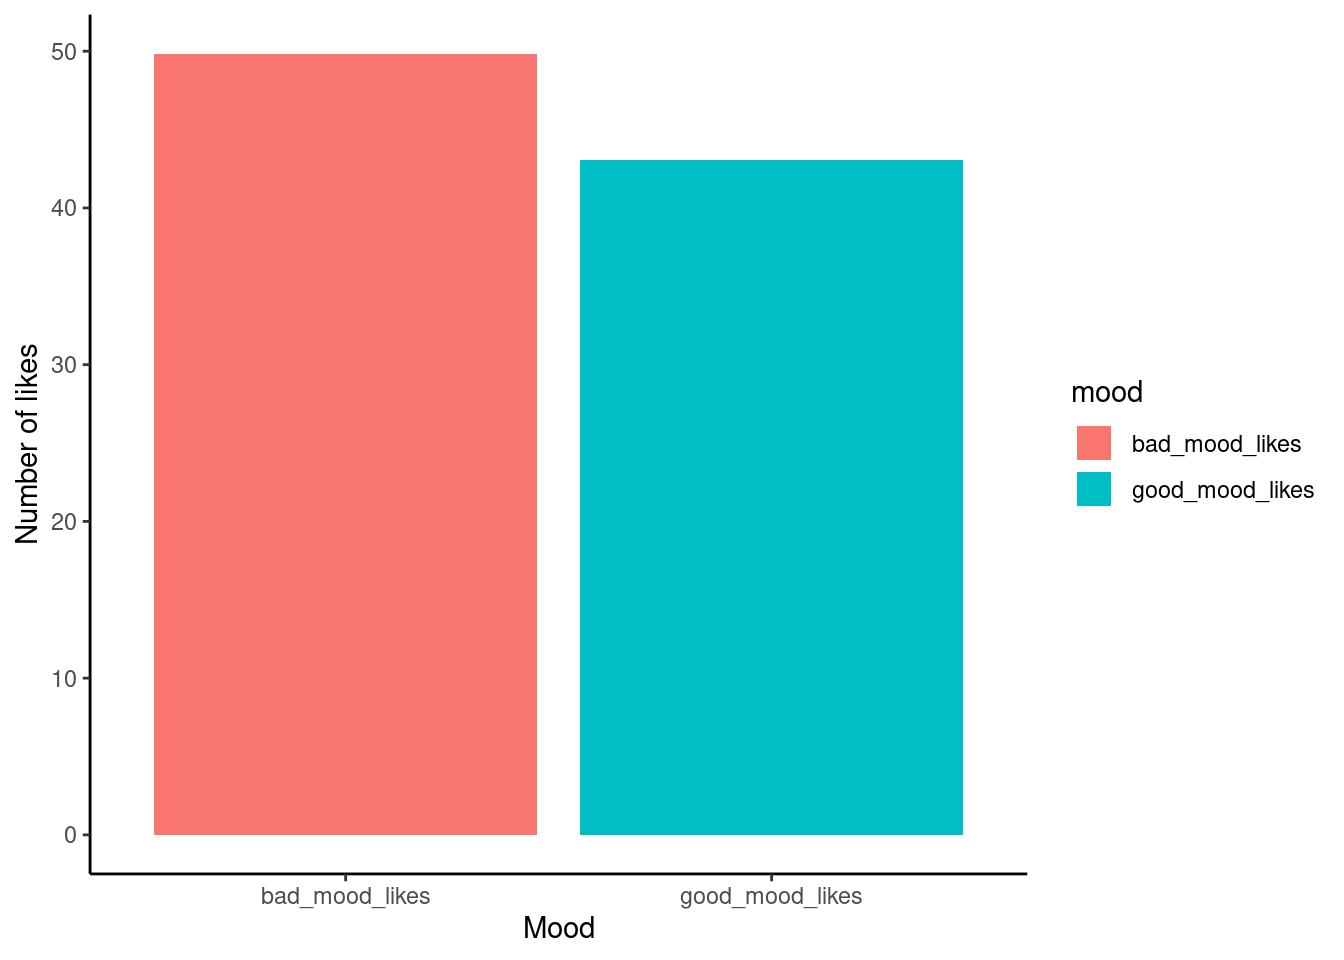
\includegraphics{_main_files/figure-latex/Activity 5-1.pdf}

\section{You are Free!}\label{you-are-free-3}

Well done you have finished for this week! There is no extension activity this week so if you have finished please confirm that you understand everything with your tutor.

\textbackslash begin\{figure\}

\{\centering \includegraphics[width=0.5\linewidth]{https://github.com/BsoCool/UNSW-PSYC2001/blob/main/All%20images%20for%20computing%20tutorials/Testing_our_first_hypothesis/Students%20leaving.gif?raw=true} 

}

\caption{Students leaving evil statistics classes}

\label{fig:unnamed-chunk-52}
\textbackslash end\{figure\}

\chapter{Testing between groups}\label{testing-between-groups}

\section{Checking installation and loading packages}\label{checking-installation-and-loading-packages-3}

As usual we first always check and load in our required packages.

\begin{Shaded}
\begin{Highlighting}[]
\CommentTok{\# Check if packages are installed, if not install.}
\ControlFlowTok{if}\NormalTok{(}\SpecialCharTok{!}\FunctionTok{require}\NormalTok{(here)) }\FunctionTok{install.packages}\NormalTok{(}\StringTok{\textquotesingle{}here\textquotesingle{}}\NormalTok{) }\CommentTok{\#checks if a package is installed and installs it if required.}
\ControlFlowTok{if}\NormalTok{(}\SpecialCharTok{!}\FunctionTok{require}\NormalTok{(tidyverse)) }\FunctionTok{install.packages}\NormalTok{(}\StringTok{\textquotesingle{}tidyverse\textquotesingle{}}\NormalTok{)}
\ControlFlowTok{if}\NormalTok{(}\SpecialCharTok{!}\FunctionTok{require}\NormalTok{(ggplot2)) }\FunctionTok{install.packages}\NormalTok{(}\StringTok{\textquotesingle{}ggplot2\textquotesingle{}}\NormalTok{)}

\FunctionTok{library}\NormalTok{(here) }\CommentTok{\#loads in the specified package}
\FunctionTok{library}\NormalTok{(tidyverse)}
\FunctionTok{library}\NormalTok{(ggplot2)}
\end{Highlighting}
\end{Shaded}

\section{Testing between groups}\label{testing-between-groups-1}

We observed last week how mood impacts active social media behaviour. However, that is not the only factor that influences social media use. For example, \href{https://academic.oup.com/pnasnexus/article/2/11/pgad357/7442564}{Sapienza et al (2023)} found that people in rural areas are more likely to use their smartphone for social media and gaming, whereas urban dwellers are more likely to use their phone for navigation and business.

However, we do not know if people living in urban and rural areas engage with social media differently, regardless of how long they spend on their chosen platforms. Today we will address this question using the \texttt{urban}, \texttt{good\_mood\_likes}, \texttt{bad\_mood\_likes}, and \texttt{followers} variables. Remember, these variables stand for the following:

\begin{itemize}
\tightlist
\item
  \texttt{urban} -- urban (1) or rural (2) area (based on postcode density)
\item
  \texttt{good\_mood\_likes} -- average number of likes made over 10 min during a good mood (from platform + diary)
\item
  \texttt{bad\_mood\_likes} -- as above, but during bad mood
\item
  \texttt{followers} -- average number of followers across platforms
\end{itemize}

\section{Activity 1 - Formulate your research question}\label{activity-1---formulate-your-research-question}

What do you think? Will urban and rural dwellers engage differently with social media? Will there be a difference in the number of likes made by people living in urban vs rural areas? Or in the number of followers people have in urban vs rural areas?

Question: What are the null hypotheses for your research questions (you should have one for `likes' and one for `followers'? What would you expect to see if your prediction is correct? Discuss this with your neighbor and your tutor.

Hint: We are going to average over the effect of mood, so we do not need to include mood in our predictions about likes.

\section{Activity 2 - Creating our likes variable}\label{activity-2---creating-our-likes-variable}

Today we will be averaging across mood to get the number of likes for urban and rural dwellers. This means we first need to create a new variable called \texttt{likes} which is the average of the likes in a good and bad mood.

We first load in our\texttt{PSYC2001\_social-media-data.csv} dataset.

\begin{Shaded}
\begin{Highlighting}[]
\NormalTok{social\_media }\OtherTok{\textless{}{-}} \FunctionTok{read.csv}\NormalTok{(}\AttributeTok{file =} \FunctionTok{here}\NormalTok{(}\StringTok{"Data"}\NormalTok{,}\StringTok{"PSYC2001\_social{-}media{-}data{-}cleaned.csv"}\NormalTok{)) }\CommentTok{\#reads in CSV files}
\end{Highlighting}
\end{Shaded}

Lets double check its the data we think it is\ldots{}

\begin{Shaded}
\begin{Highlighting}[]
\FunctionTok{head}\NormalTok{(social\_media, }\DecValTok{10}\NormalTok{) }\CommentTok{\# you can even say how many lines you want to see! Try changing the number, and see what happens.}
\end{Highlighting}
\end{Shaded}

\begin{verbatim}
##     X  id  age time_on_social urban good_mood_likes bad_mood_likes followers
## 1   1  S1 15.2           3.06     1            22.8           46.5     173.3
## 2   2  S2 16.0           2.18     1            46.0           48.3     144.3
## 3   3  S3 16.8           1.92     1            50.8           46.1      76.5
## 4   4  S4 15.6           2.61     1            29.9           29.2     171.7
## 5   5  S5 17.1           3.24     1            37.1           52.4     109.5
## 6   6  S6 15.7           2.44     1            26.9           20.2     157.5
## 7   7  S7 19.7           1.46     1            14.8           35.1     166.9
## 8   8  S8 18.6           1.52     1            26.0           35.8     109.6
## 9   9  S9 19.6           1.92     1             6.5           12.2     253.4
## 10 10 S10 15.5           2.10     1            45.7           32.8      77.2
##    polit_informed polit_campaign polit_activism
## 1             2.3            3.2            3.6
## 2             1.6            2.2            2.6
## 3             1.9            2.7            3.0
## 4             1.6            2.3            2.6
## 5             2.0            2.9            3.3
## 6             2.4            3.4            3.9
## 7             1.7            2.4            2.7
## 8             1.6            2.2            2.6
## 9             1.5            2.1            2.4
## 10            2.2            3.1            3.5
\end{verbatim}

Are you able to fill the code below using the \texttt{mutate()} function to create this new `likes' variable?

Hint: The average of likes is \texttt{(good\_mood\_likes\ +\ bad\_mood\_likes)/2}

\begin{Shaded}
\begin{Highlighting}[]
\NormalTok{social\_media\_likes }\OtherTok{\textless{}{-}}\NormalTok{ social\_media }\SpecialCharTok{\%\textgreater{}\%} 
  \FunctionTok{mutate}\NormalTok{(}\AttributeTok{likes =}\NormalTok{(bad\_mood\_likes }\SpecialCharTok{+}\NormalTok{ good\_mood\_likes)}\SpecialCharTok{/}\DecValTok{2}\NormalTok{ ) }\SpecialCharTok{\%\textgreater{}\%} \CommentTok{\#create a new column with specified values}
  \FunctionTok{select}\NormalTok{(id, urban, likes, followers) }\CommentTok{\#keep specified columns in dataframe}

\FunctionTok{head}\NormalTok{(social\_media\_likes)}
\end{Highlighting}
\end{Shaded}

\begin{verbatim}
##   id urban likes followers
## 1 S1     1 34.65     173.3
## 2 S2     1 47.15     144.3
## 3 S3     1 48.45      76.5
## 4 S4     1 29.55     171.7
## 5 S5     1 44.75     109.5
## 6 S6     1 23.55     157.5
\end{verbatim}

\section{Wrangling our data}\label{wrangling-our-data}

Now that we have this object it is important to check the format of the data. Lets use the \texttt{str()} function that we learned about in the \hyperref[importing-your-data-in-r]{second tutorial} to do this.

\begin{Shaded}
\begin{Highlighting}[]
\FunctionTok{str}\NormalTok{(social\_media\_likes) }\CommentTok{\#provides a summary of the data structure.}
\end{Highlighting}
\end{Shaded}

\begin{verbatim}
## 'data.frame':    60 obs. of  4 variables:
##  $ id       : chr  "S1" "S2" "S3" "S4" ...
##  $ urban    : int  1 1 1 1 1 1 1 1 1 1 ...
##  $ likes    : num  34.6 47.1 48.5 29.5 44.8 ...
##  $ followers: num  173.3 144.3 76.5 171.7 109.5 ...
\end{verbatim}

First we can see that having the values in \texttt{urban} are coded as either 1 (urban) or 2 (rural). Lets change this so that instead of using numbers we use the actual descriptions of urban and rural. It is surprisingly difficult to remember what 1 and 2 stand for once you come to look at your graphs. Life will be much easier if we can see what 1 and 2 stand for instead. To do this we will use the \texttt{mutate()} function with the \texttt{case\_when()} function which replaces (or creates) specific values in a variable with new ones.

\begin{Shaded}
\begin{Highlighting}[]
\NormalTok{social\_media\_likes }\OtherTok{\textless{}{-}}\NormalTok{ social\_media\_likes }\SpecialCharTok{\%\textgreater{}\%} 
  \FunctionTok{mutate}\NormalTok{(}\AttributeTok{urban =} \FunctionTok{case\_when}\NormalTok{(urban }\SpecialCharTok{==} \DecValTok{1} \SpecialCharTok{\textasciitilde{}} \StringTok{"urban"}\NormalTok{, }
\NormalTok{                           urban }\SpecialCharTok{==} \DecValTok{2} \SpecialCharTok{\textasciitilde{}} \StringTok{"rural"}\NormalTok{)) }\CommentTok{\#case\_when uses if\_else logic to replace values with specified values if the cases match.}

\FunctionTok{str}\NormalTok{(social\_media\_likes)}
\end{Highlighting}
\end{Shaded}

\begin{verbatim}
## 'data.frame':    60 obs. of  4 variables:
##  $ id       : chr  "S1" "S2" "S3" "S4" ...
##  $ urban    : chr  "urban" "urban" "urban" "urban" ...
##  $ likes    : num  34.6 47.1 48.5 29.5 44.8 ...
##  $ followers: num  173.3 144.3 76.5 171.7 109.5 ...
\end{verbatim}

We can see that \texttt{urban} is now classed as a \texttt{chr} (character) but we will eventually need to split our graphs by \texttt{urban}. This means that \texttt{urban} should be a factor instead. (Also, urban is a factor in the experiment, so lets keep it consistent). Luckily, we can change this easily by using \texttt{as.factor()} within the \texttt{mutate()} function. The \texttt{as.factor()} function is used to convert other datatypes to factors !

\begin{Shaded}
\begin{Highlighting}[]
\NormalTok{social\_media\_likes }\OtherTok{\textless{}{-}}\NormalTok{ social\_media\_likes }\SpecialCharTok{\%\textgreater{}\%} 
  \FunctionTok{mutate}\NormalTok{(}\AttributeTok{urban =} \FunctionTok{as.factor}\NormalTok{(urban))}

\FunctionTok{str}\NormalTok{(social\_media\_likes)}
\end{Highlighting}
\end{Shaded}

\begin{verbatim}
## 'data.frame':    60 obs. of  4 variables:
##  $ id       : chr  "S1" "S2" "S3" "S4" ...
##  $ urban    : Factor w/ 2 levels "rural","urban": 2 2 2 2 2 2 2 2 2 2 ...
##  $ likes    : num  34.6 47.1 48.5 29.5 44.8 ...
##  $ followers: num  173.3 144.3 76.5 171.7 109.5 ...
\end{verbatim}

The data is now in a format that we should be able to easily visualise it and conduct our statistical tests. Well done !

\textbackslash begin\{figure\}

\{\centering \includegraphics[width=0.5\linewidth]{https://github.com/BsoCool/UNSW-PSYC2001/blob/main/All%20images%20for%20computing%20tutorials/Testing_between_groups/What%20it%20feels%20like%20to%20explain%20this%20section.gif?raw=true} 

}

\caption{What it feels like teaching this section}

\label{fig:unnamed-chunk-59}
\textbackslash end\{figure\}

\section{Activity 3 - Visualising our data before analysis}\label{activity-3---visualising-our-data-before-analysis}

We're now going to look at the data in 2 ways. First, we're going to look at how the data is distributed across all participants, so that we can check if the data meets our assumptions about normality. Second, we are going to plot our dependent variables (\texttt{likes}, \texttt{followers}) by group, to gain a visual understanding for what group differences might look like, if they exist.

Here, we create a density plot for \texttt{likes}.

\begin{Shaded}
\begin{Highlighting}[]
\NormalTok{social\_media\_likes }\SpecialCharTok{\%\textgreater{}\%} 
  \FunctionTok{ggplot}\NormalTok{(}\FunctionTok{aes}\NormalTok{(}\AttributeTok{x =}\NormalTok{ likes)) }\SpecialCharTok{+}
  \FunctionTok{geom\_density}\NormalTok{(}\AttributeTok{linewidth =} \DecValTok{2}\NormalTok{, }\AttributeTok{colour =} \StringTok{"blue"}\NormalTok{) }\SpecialCharTok{+} \CommentTok{\#the argument linewidth is used to alter the size of the density line. }
  \FunctionTok{labs}\NormalTok{(}\AttributeTok{x =} \StringTok{"Number of Likes"}\NormalTok{, }\AttributeTok{y =} \StringTok{"Density"}\NormalTok{) }\SpecialCharTok{+}
  \FunctionTok{theme\_classic}\NormalTok{() }
\end{Highlighting}
\end{Shaded}

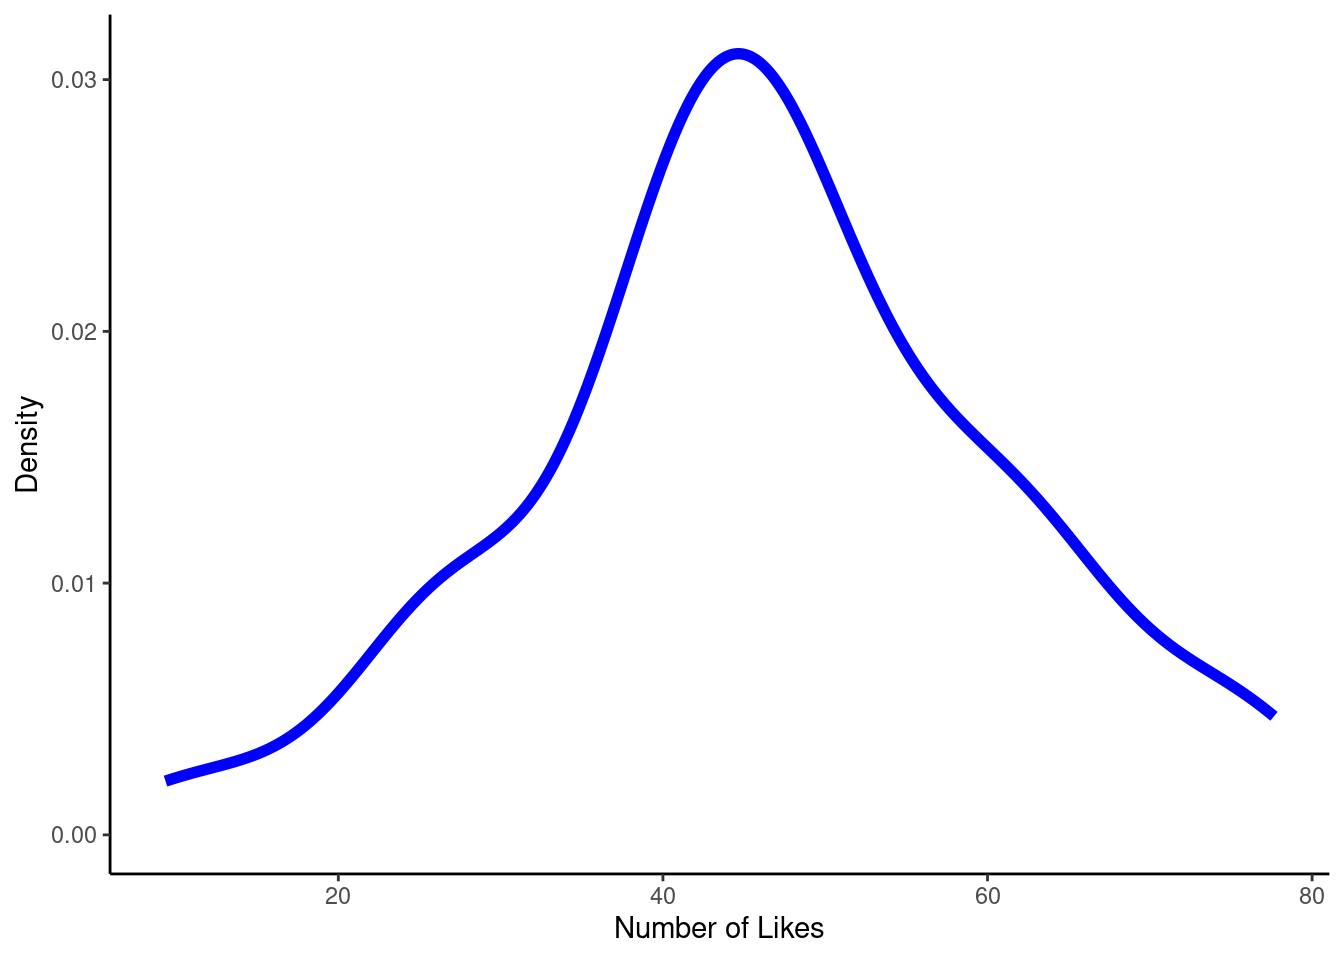
\includegraphics{_main_files/figure-latex/Density plot of likes-1.pdf}

Info: We use a new argument here \texttt{linewidth} to control the size of the density line.

Now, can you make a density plot for \texttt{followers}? Go on, you are a coder and you are strong.

\begin{Shaded}
\begin{Highlighting}[]
\NormalTok{social\_media\_likes }\SpecialCharTok{\%\textgreater{}\%} 
  \FunctionTok{ggplot}\NormalTok{(}\FunctionTok{aes}\NormalTok{(}\AttributeTok{x =}\NormalTok{ followers)) }\SpecialCharTok{+} 
  \FunctionTok{geom\_density}\NormalTok{(}\AttributeTok{linewidth =} \DecValTok{2}\NormalTok{, }\AttributeTok{colour =} \StringTok{"orange"}\NormalTok{) }\SpecialCharTok{+}
  \FunctionTok{labs}\NormalTok{(}\AttributeTok{x =} \StringTok{"Number of followers"}\NormalTok{, }\AttributeTok{y =} \StringTok{"Density"}\NormalTok{) }\SpecialCharTok{+}
  \FunctionTok{theme\_classic}\NormalTok{() }
\end{Highlighting}
\end{Shaded}

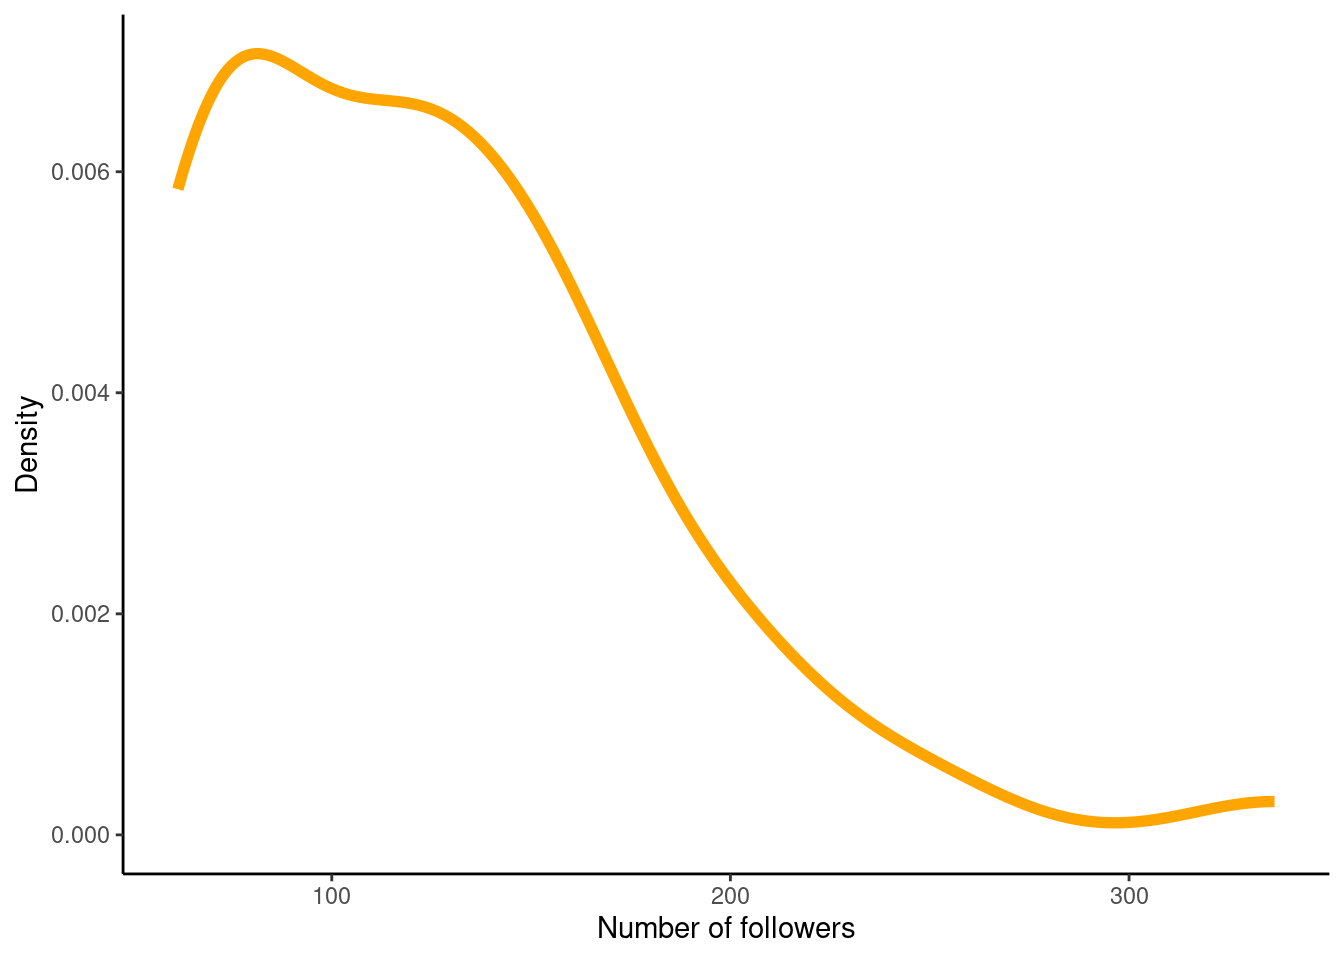
\includegraphics{_main_files/figure-latex/Density plot of followers-1.pdf}

Question: Do \texttt{likes} and \texttt{followers} look normally distributed to you? Why might the data be shaped how they are for each variable?

Question: What impact does your new understanding of the data have on your analysis, if any?

\section{Activity 4 - Visualising group differences}\label{activity-4---visualising-group-differences}

Now we are going to make some density plots and boxplots, split by the urban factor so that we can see the group differences.

Are you able to help with this?

Hint: Use the \texttt{colour} argument in \texttt{aes()} to split the plot by \texttt{Urban}

\begin{Shaded}
\begin{Highlighting}[]
\NormalTok{social\_media\_likes }\SpecialCharTok{\%\textgreater{}\%} 
  \FunctionTok{ggplot}\NormalTok{(}\FunctionTok{aes}\NormalTok{(}\AttributeTok{x =}\NormalTok{ likes, }\AttributeTok{colour =}\NormalTok{ urban)) }\SpecialCharTok{+}
  \FunctionTok{geom\_density}\NormalTok{(}\AttributeTok{linewidth =} \DecValTok{2}\NormalTok{) }\SpecialCharTok{+}
  \FunctionTok{labs}\NormalTok{(}\AttributeTok{x =} \StringTok{"Number of Likes"}\NormalTok{, }\AttributeTok{y =} \StringTok{"Density"}\NormalTok{) }\SpecialCharTok{+}
  \FunctionTok{scale\_colour\_manual}\NormalTok{(}\AttributeTok{values =} \FunctionTok{c}\NormalTok{(}\AttributeTok{rural =} \StringTok{"purple"}\NormalTok{, }\AttributeTok{urban =} \StringTok{"green"}\NormalTok{)) }\SpecialCharTok{+} \CommentTok{\#manually define colours of specific parts of a graph}
  \FunctionTok{theme\_classic}\NormalTok{() }
\end{Highlighting}
\end{Shaded}

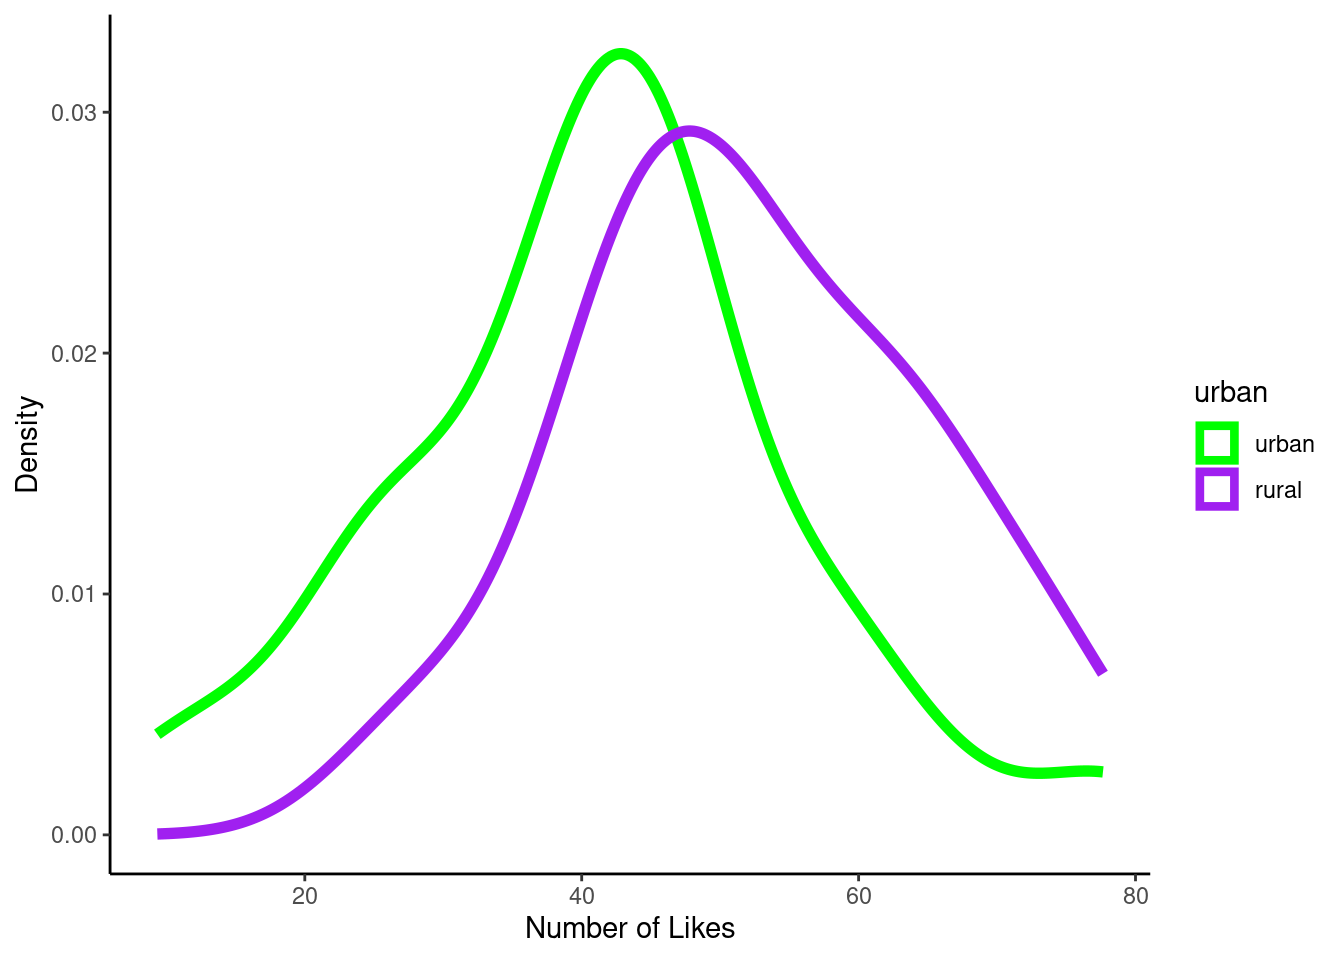
\includegraphics{_main_files/figure-latex/Density plot likes split by urban-1.pdf}

\begin{Shaded}
\begin{Highlighting}[]
\NormalTok{social\_media\_likes }\SpecialCharTok{\%\textgreater{}\%} 
  \FunctionTok{ggplot}\NormalTok{(}\FunctionTok{aes}\NormalTok{(}\AttributeTok{x =}\NormalTok{ followers, }\AttributeTok{colour =}\NormalTok{ urban)) }\SpecialCharTok{+}
  \FunctionTok{geom\_density}\NormalTok{(}\AttributeTok{linewidth =} \DecValTok{2}\NormalTok{) }\SpecialCharTok{+}
  \FunctionTok{labs}\NormalTok{(}\AttributeTok{x =} \StringTok{"Number of Followers"}\NormalTok{, }\AttributeTok{y =} \StringTok{"Density"}\NormalTok{) }\SpecialCharTok{+}
  \FunctionTok{scale\_colour\_manual}\NormalTok{(}\AttributeTok{values =} \FunctionTok{c}\NormalTok{(}\AttributeTok{rural =} \StringTok{"purple"}\NormalTok{, }\AttributeTok{urban =} \StringTok{"green"}\NormalTok{)) }\SpecialCharTok{+} \CommentTok{\#manually define colours of specific parts of a graph}
  \FunctionTok{theme\_classic}\NormalTok{() }
\end{Highlighting}
\end{Shaded}

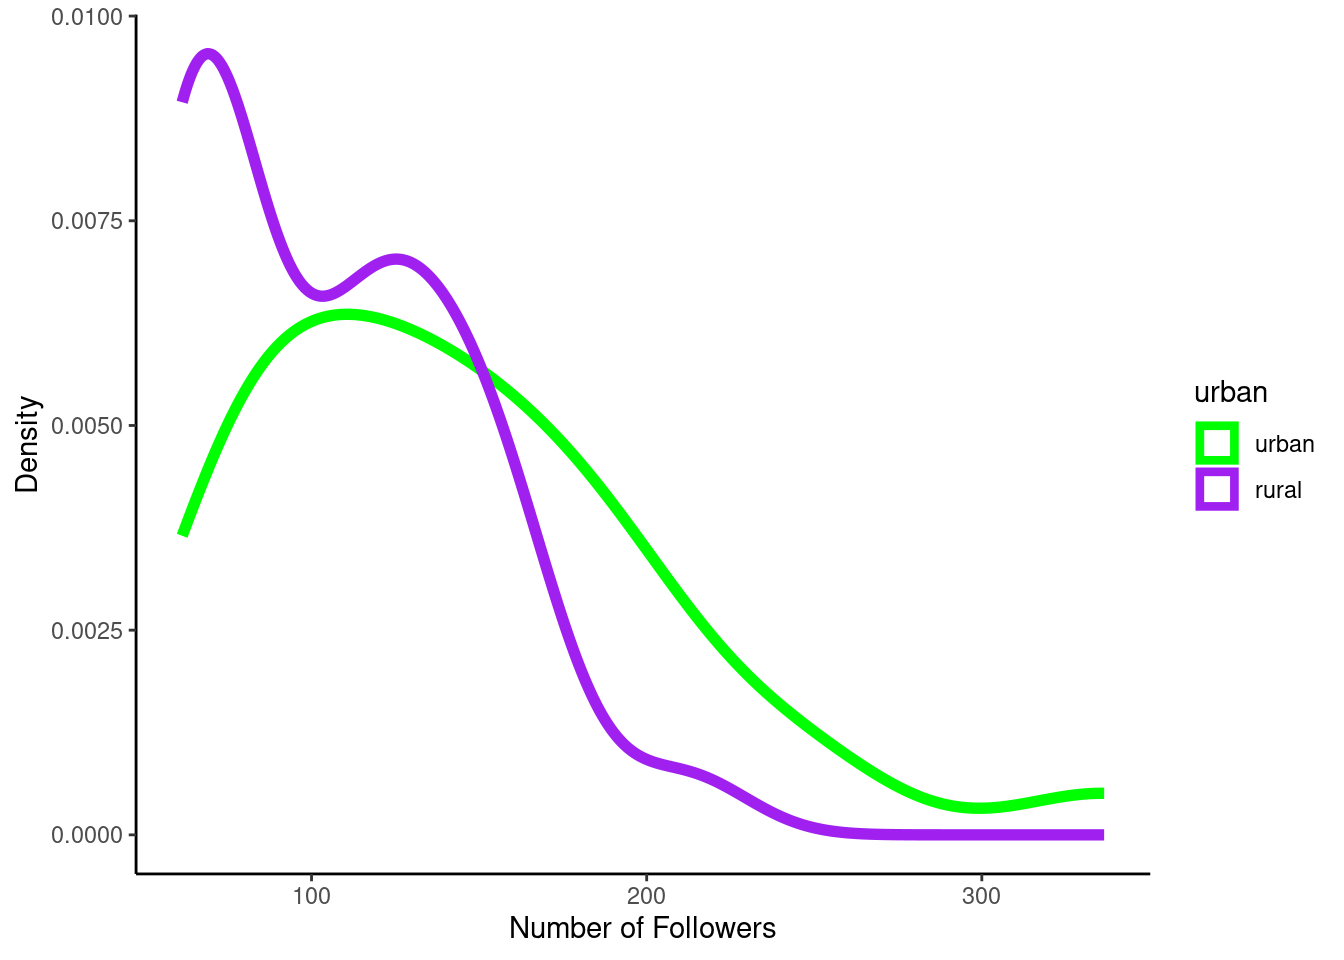
\includegraphics{_main_files/figure-latex/Density plot followers split by urban-1.pdf}

Info: We are using a new function here called \texttt{scale\_colour\_manual()}. This allows you manually define the colours of specific parts of a graph. Here we have used it to define colours for specific groups.

This is not the only way we may want to view the group differences in likes and followers. Using a grouped boxplot can be a handy way at looking at how groups differ from each other.

\begin{Shaded}
\begin{Highlighting}[]
\NormalTok{social\_media\_likes }\SpecialCharTok{\%\textgreater{}\%} 
  \FunctionTok{ggplot}\NormalTok{(}\FunctionTok{aes}\NormalTok{(}\AttributeTok{y =}\NormalTok{ likes, }\AttributeTok{colour =}\NormalTok{ urban, }\AttributeTok{x =}\NormalTok{ urban)) }\SpecialCharTok{+}
  \FunctionTok{geom\_boxplot}\NormalTok{() }\SpecialCharTok{+}
  \FunctionTok{labs}\NormalTok{(}\AttributeTok{x =} \StringTok{" "}\NormalTok{, }\AttributeTok{y =} \StringTok{"Number of Likes"}\NormalTok{) }\SpecialCharTok{+}
  \FunctionTok{scale\_colour\_manual}\NormalTok{(}\AttributeTok{values =} \FunctionTok{c}\NormalTok{(}\AttributeTok{rural =} \StringTok{"purple"}\NormalTok{, }\AttributeTok{urban =} \StringTok{"green"}\NormalTok{)) }\SpecialCharTok{+} \CommentTok{\#manually define colours of specific parts of a graph}
  \FunctionTok{theme\_classic}\NormalTok{() }
\end{Highlighting}
\end{Shaded}

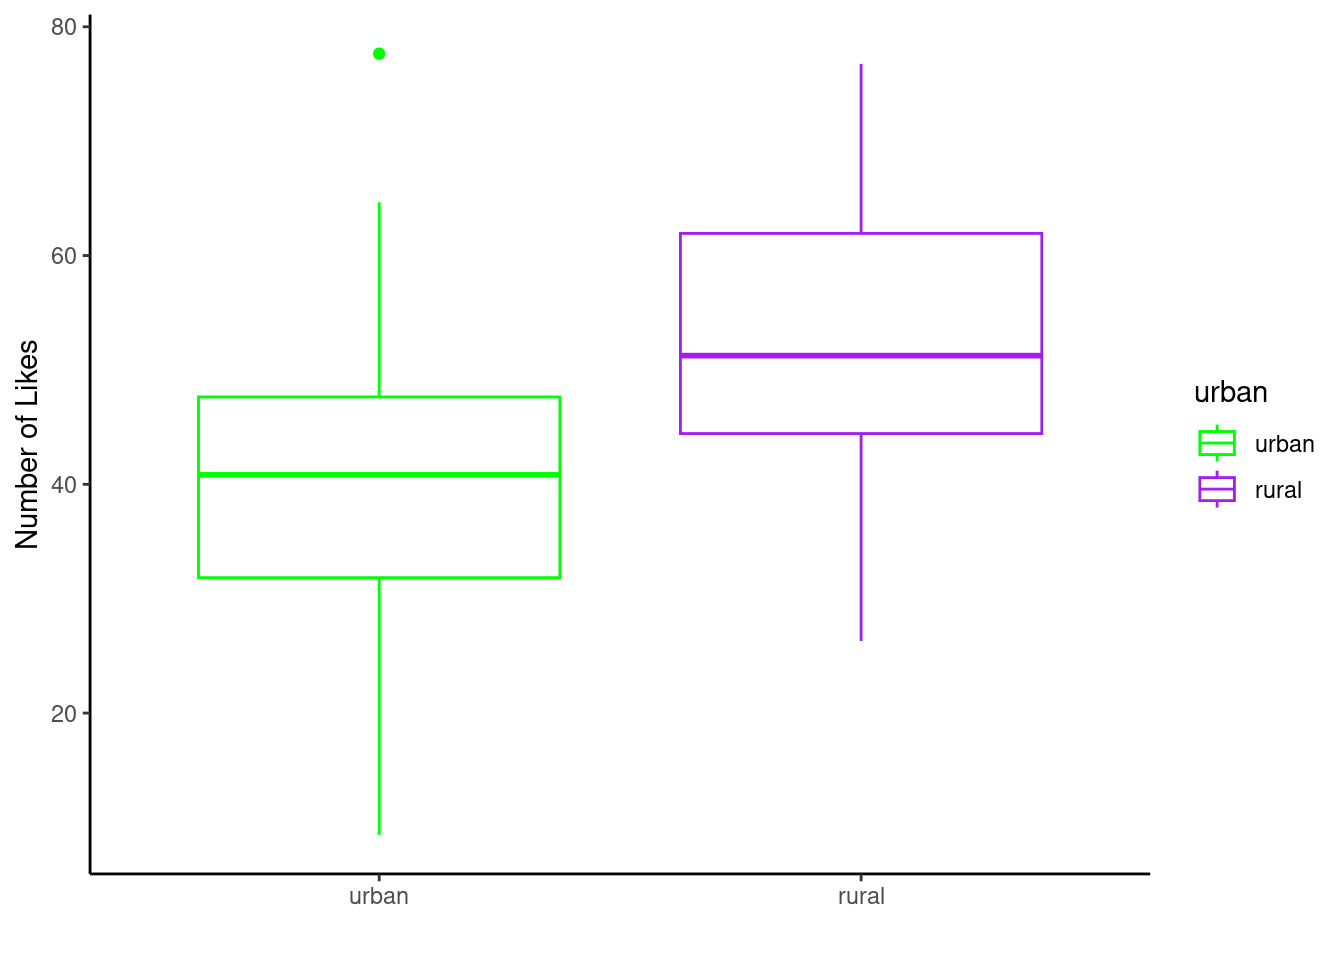
\includegraphics{_main_files/figure-latex/Boxplot of likes split by urban-1.pdf}

Can you change the code below so that the x-axis has a label, and the y-axis label is correct?

\begin{Shaded}
\begin{Highlighting}[]
\NormalTok{social\_media\_likes }\SpecialCharTok{\%\textgreater{}\%} 
  \FunctionTok{ggplot}\NormalTok{(}\FunctionTok{aes}\NormalTok{(}\AttributeTok{y =}\NormalTok{ followers, }\AttributeTok{colour =}\NormalTok{ urban, }\AttributeTok{x =}\NormalTok{ urban)) }\SpecialCharTok{+}
  \FunctionTok{geom\_boxplot}\NormalTok{() }\SpecialCharTok{+}
  \FunctionTok{labs}\NormalTok{(}\AttributeTok{x =} \StringTok{""}\NormalTok{, }\AttributeTok{y =} \StringTok{"Number of Likes"}\NormalTok{) }\SpecialCharTok{+}
  \FunctionTok{scale\_colour\_manual}\NormalTok{(}\AttributeTok{values =} \FunctionTok{c}\NormalTok{(}\AttributeTok{rural =} \StringTok{"purple"}\NormalTok{, }\AttributeTok{urban =} \StringTok{"green"}\NormalTok{)) }\SpecialCharTok{+} \CommentTok{\#manually define colours of specific parts of a graph}
  \FunctionTok{theme\_classic}\NormalTok{() }
\end{Highlighting}
\end{Shaded}

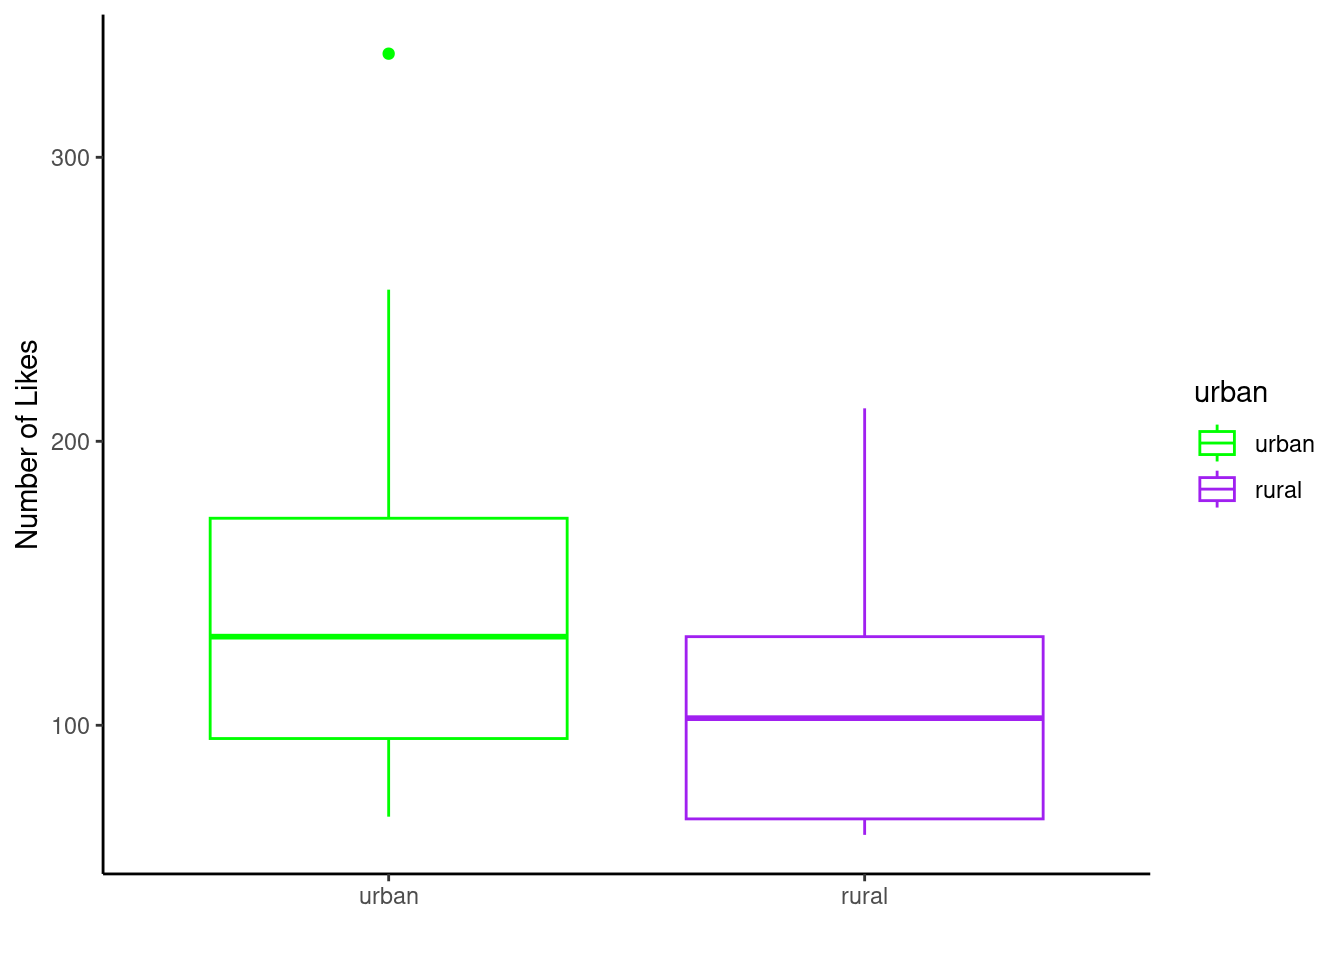
\includegraphics{_main_files/figure-latex/Boxplot of followers split by urban-1.pdf}

Question: What do you think the data suggest about the group differences for \texttt{likes} and \texttt{followers}? Was it in-line with your predictions from activity 1? Are there any caveats or reasons to be cautious about your interpretations?

\section{Activity 5 - Descriptive statistics}\label{activity-5---descriptive-statistics}

It is important to generate descriptive statistics before our t-test. Are you able to fill in the code below to generate the mean and standard deviation of likes and followers for urban and rural dwellers ?

\begin{Shaded}
\begin{Highlighting}[]
\NormalTok{social\_media\_descriptives }\OtherTok{\textless{}{-}}\NormalTok{ social\_media\_likes }\SpecialCharTok{\%\textgreater{}\%} 
  \FunctionTok{group\_by}\NormalTok{(urban) }\SpecialCharTok{\%\textgreater{}\%} 
  \FunctionTok{summarise}\NormalTok{(}
    \AttributeTok{mean\_followers =} \FunctionTok{mean}\NormalTok{(followers),}
    \AttributeTok{mean\_likes =} \FunctionTok{mean}\NormalTok{(likes),}
    \AttributeTok{sd\_follower =} \FunctionTok{sd}\NormalTok{(followers),}
    \AttributeTok{sd\_likes =} \FunctionTok{sd}\NormalTok{(likes)}
\NormalTok{  )}

\FunctionTok{head}\NormalTok{(social\_media\_descriptives)}
\end{Highlighting}
\end{Shaded}

\begin{verbatim}
## # A tibble: 2 x 5
##   urban mean_followers mean_likes sd_follower sd_likes
##   <fct>          <dbl>      <dbl>       <dbl>    <dbl>
## 1 rural           106.       52.1        40.9     12.7
## 2 urban           144.       40.8        62.0     14.5
\end{verbatim}

\section{Independent samples t-test}\label{independent-samples-t-test}

We now want to learn whether we have evidence for differences between urban and rural dwellers on the `likes' and `followers' variables.

\section{Activity 6 - Undertaking an independent samples t-test}\label{activity-6---undertaking-an-independent-samples-t-test}

Can you work out how to perform an independent samples t-test for these variables ?

Hint: Use the \texttt{t.test()} function from the tutorial last week and pay attention to the `paired' argument !

\begin{Shaded}
\begin{Highlighting}[]
\FunctionTok{t.test}\NormalTok{(}\AttributeTok{formula =}\NormalTok{ likes }\SpecialCharTok{\textasciitilde{}}\NormalTok{ urban, }\AttributeTok{data =}\NormalTok{ social\_media\_likes, }\AttributeTok{var.equal =} \ConstantTok{TRUE}\NormalTok{, }\AttributeTok{paired =} \ConstantTok{FALSE}\NormalTok{)}
\end{Highlighting}
\end{Shaded}

\begin{verbatim}
## 
##  Two Sample t-test
## 
## data:  likes by urban
## t = 3.2184, df = 58, p-value = 0.002112
## alternative hypothesis: true difference in means between group rural and group urban is not equal to 0
## 95 percent confidence interval:
##   4.273656 18.336344
## sample estimates:
## mean in group rural mean in group urban 
##            52.09333            40.78833
\end{verbatim}

\begin{Shaded}
\begin{Highlighting}[]
\FunctionTok{t.test}\NormalTok{(}\AttributeTok{formula =}\NormalTok{ followers }\SpecialCharTok{\textasciitilde{}}\NormalTok{ urban, }\AttributeTok{data =}\NormalTok{ social\_media\_likes, }\AttributeTok{var.equal =} \ConstantTok{TRUE}\NormalTok{, }\AttributeTok{paired =} \ConstantTok{FALSE}\NormalTok{)}
\end{Highlighting}
\end{Shaded}

\begin{verbatim}
## 
##  Two Sample t-test
## 
## data:  followers by urban
## t = -2.8182, df = 58, p-value = 0.006595
## alternative hypothesis: true difference in means between group rural and group urban is not equal to 0
## 95 percent confidence interval:
##  -65.40138 -11.07862
## sample estimates:
## mean in group rural mean in group urban 
##            105.6367            143.8767
\end{verbatim}

Question: Discuss the output of this independent t-tests, what does it tell you about the differences between urban and rural dwellers and how they use social media ? Is it what you expected when you formulated your hypotheses?

\textbackslash begin\{figure\}

\{\centering \includegraphics[width=0.5\linewidth]{https://github.com/BsoCool/UNSW-PSYC2001/blob/main/All%20images%20for%20computing%20tutorials/Testing_between_groups/Exams%20are%20hard.jpg?raw=true} 

}

\caption{Exams are hard}

\label{fig:unnamed-chunk-63}
\textbackslash end\{figure\}

\section{Writing up results and conclusions}\label{writing-up-results-and-conclusions-1}

Lets have a go at writing up the results and conclusions for this independent samples t-test.

Results: An independent samples t-test indicated that the number of likes was greater for rural (M = 52.1 , SD = 12.7) compared to urban dwellers (M = 40.8 , SD = 14.5) and this difference was statistically significant (t(58) = 3.22, p = 0.002). Conversely, the number of followers was greater for urban (Mean = 143.9, SD = 62.0) than for urban dwellers (M = 105.6, SD = 40.9) which was statistically significant (t(58) = 2.82, p = 0.007).

Given these results have a go at writing up our conclusions.

Conclusions: Your conclusion will go here !

\section{You are Free!}\label{you-are-free-4}

Well done ! This computing tutorial is now over. Make sure to thank your tutor for another amazing class full of wonderful statistics and learning !

\textbackslash begin\{figure\}

\{\centering \includegraphics[width=0.5\linewidth]{https://github.com/BsoCool/UNSW-PSYC2001/blob/main/All%20images%20for%20computing%20tutorials/Testing_between_groups/Everyone%20loves%20statistics.jpg?raw=true} 

}

\caption{Everyone loves statistics ?}

\label{fig:unnamed-chunk-64}
\textbackslash end\{figure\}

\chapter{You got the power !}\label{you-got-the-power}

This week, we are going to explore how improving our statistical power changes our ability to detect effects, if they exist.

\section{Checking installation and loading packages}\label{checking-installation-and-loading-packages-4}

As usual we first always check and load in our required packages.

\begin{Shaded}
\begin{Highlighting}[]
\CommentTok{\# Check if packages are installed, if not install.}
\ControlFlowTok{if}\NormalTok{(}\SpecialCharTok{!}\FunctionTok{require}\NormalTok{(here)) }\FunctionTok{install.packages}\NormalTok{(}\StringTok{\textquotesingle{}here\textquotesingle{}}\NormalTok{) }\CommentTok{\#checks if a package is installed and installs it if required.}
\ControlFlowTok{if}\NormalTok{(}\SpecialCharTok{!}\FunctionTok{require}\NormalTok{(tidyverse)) }\FunctionTok{install.packages}\NormalTok{(}\StringTok{\textquotesingle{}tidyverse\textquotesingle{}}\NormalTok{)}
\ControlFlowTok{if}\NormalTok{(}\SpecialCharTok{!}\FunctionTok{require}\NormalTok{(ggplot2)) }\FunctionTok{install.packages}\NormalTok{(}\StringTok{\textquotesingle{}ggplot2\textquotesingle{}}\NormalTok{)}

\FunctionTok{library}\NormalTok{(here) }\CommentTok{\#loads in the specified package}
\FunctionTok{library}\NormalTok{(tidyverse)}
\FunctionTok{library}\NormalTok{(ggplot2)}
\end{Highlighting}
\end{Shaded}

\section{Key power facts:}\label{key-power-facts}

\begin{enumerate}
\def\labelenumi{\arabic{enumi}.}
\item
  We can never know for sure what size our effect is going to be -- unless we measured the entire population of interest -- which is quite often THE ENTIRE HUMAN SPECIES. That would be a HUUUUUGE experiment. This means we have to make a theoretical or educated guess, and power our study accordingly.
\item
  The effect size we are hunting depends on the nature of the effect, not the size experiment we want to run. For example, the effect of getting the right nutrients on height is the same, regardless of how many people we sample in our experiment.
\end{enumerate}

\textbf{Therefore}: our job as experimenters is to make the most educated guess that we can about the effect size we are looking for, and make sure our study is appropriately powered to give us the best chance to detect it, \textbf{if it even exists.}

The \textbf{best chance we have to change statistical power is to change our sample size.}

\section{Simulating sample sizes}\label{simulating-sample-sizes}

In this first exercise we are going to simulate the impact of sample size on our experiment results using the \texttt{PSYC2001\_global-time-on-social-data.csv}. We will learn about influence of sample size on \textbf{effect size and p value} using the \texttt{mean\_time\_on\_social} variable. Remember, that this variables stands for the following:

\begin{itemize}
\tightlist
\item
  \texttt{mean\_time\_on\_social} -- average hours/day on social media per experiment (self-report diary)
\end{itemize}

\section{Installing and loading new packages we will be using today}\label{installing-and-loading-new-packages-we-will-be-using-today}

We will be using two new packages today. The \texttt{pwr} package to complete power calculations and the \texttt{effsize} package to generate effect sizes. Please run the code to install and load these packages.

\begin{Shaded}
\begin{Highlighting}[]
\ControlFlowTok{if}\NormalTok{(}\SpecialCharTok{!}\FunctionTok{require}\NormalTok{(effsize)) }\FunctionTok{install.packages}\NormalTok{(}\StringTok{\textquotesingle{}effsize\textquotesingle{}}\NormalTok{)}
\ControlFlowTok{if}\NormalTok{(}\SpecialCharTok{!}\FunctionTok{require}\NormalTok{(pwr)) }\FunctionTok{install.packages}\NormalTok{(}\StringTok{"pwr"}\NormalTok{)}

\FunctionTok{library}\NormalTok{(pwr)}
\FunctionTok{library}\NormalTok{(effsize)}
\end{Highlighting}
\end{Shaded}

\section{Activity 1 - Simulating data}\label{activity-1---simulating-data}

Before we can simulate data we first need to load in our dataset. Can you help with this ?

\begin{Shaded}
\begin{Highlighting}[]
\CommentTok{\#Use the read.csv() and here() functions to read in the dataset.}

\NormalTok{global\_social\_media }\OtherTok{\textless{}{-}} \FunctionTok{read.csv}\NormalTok{(}\AttributeTok{file =} \FunctionTok{here}\NormalTok{(}\StringTok{"Data"}\NormalTok{,}\StringTok{"PSYC2001\_global{-}time{-}on{-}social{-}data.csv"}\NormalTok{))}
\end{Highlighting}
\end{Shaded}

To simulate our data we will be using our friend the \texttt{sample()} function from the previous tutorial. If you need a reminder on the usage of this function please click \hyperref[vectors-and-the-sample-function]{here} or use the \texttt{?} syntax.

Now that you are an expert on this function are you able to sample data for n = 10, n= 30, n= 50, n = 100, n= 200 and n = 500 ? Have a try at filling in the code block below:

\begin{Shaded}
\begin{Highlighting}[]
\FunctionTok{set.seed}\NormalTok{(}\DecValTok{1}\NormalTok{) }\CommentTok{\#ensures we always get the same result from sampling ! }

\NormalTok{sample\_10 }\OtherTok{\textless{}{-}} \FunctionTok{sample}\NormalTok{(global\_social\_media}\SpecialCharTok{$}\NormalTok{mean\_time\_on\_social, }\AttributeTok{size =} \DecValTok{10}\NormalTok{)}
\NormalTok{sample\_30 }\OtherTok{\textless{}{-}}\FunctionTok{sample}\NormalTok{(global\_social\_media}\SpecialCharTok{$}\NormalTok{mean\_time\_on\_social, }\AttributeTok{size =} \DecValTok{30}\NormalTok{)}
\NormalTok{sample\_50 }\OtherTok{\textless{}{-}}\FunctionTok{sample}\NormalTok{(global\_social\_media}\SpecialCharTok{$}\NormalTok{mean\_time\_on\_social, }\AttributeTok{size =} \DecValTok{50}\NormalTok{)}
\NormalTok{sample\_100 }\OtherTok{\textless{}{-}}\FunctionTok{sample}\NormalTok{(global\_social\_media}\SpecialCharTok{$}\NormalTok{mean\_time\_on\_social, }\AttributeTok{size =} \DecValTok{100}\NormalTok{)}
\NormalTok{sample\_200 }\OtherTok{\textless{}{-}}\FunctionTok{sample}\NormalTok{(global\_social\_media}\SpecialCharTok{$}\NormalTok{mean\_time\_on\_social, }\AttributeTok{size =} \DecValTok{200}\NormalTok{)}
\NormalTok{sample\_500 }\OtherTok{\textless{}{-}}\FunctionTok{sample}\NormalTok{(global\_social\_media}\SpecialCharTok{$}\NormalTok{mean\_time\_on\_social, }\AttributeTok{size =} \DecValTok{500}\NormalTok{)}
\end{Highlighting}
\end{Shaded}

Now that we have got our simulated data we are going to test whether the sample of \texttt{time-on-social} data is on average, above the international average of 2.2 hours. To do this we can run a one sample t-test against the test value of 2.2 for each of our simulated datasets. This will return a \textbf{p value} that we can use later on. We also want to get the \textbf{effect size} for each of these t-tests. To do this we will also using the \texttt{cohen.d()} function from the \texttt{effsize} package. It has the same arguments as the \texttt{t.test()} function as you will see below.

\section{Activity 2 - Conducting t tests and effect sizes.}\label{activity-2---conducting-t-tests-and-effect-sizes.}

Are you able to fill in the code below to help with this ?

\begin{Shaded}
\begin{Highlighting}[]
\NormalTok{t\_test\_10 }\OtherTok{\textless{}{-}} \FunctionTok{t.test}\NormalTok{(sample\_10 }\SpecialCharTok{\textasciitilde{}} \DecValTok{1}\NormalTok{, }\AttributeTok{mu =} \FloatTok{2.2}\NormalTok{)}
\NormalTok{eff\_size\_10 }\OtherTok{\textless{}{-}} \FunctionTok{cohen.d}\NormalTok{(sample\_10 }\SpecialCharTok{\textasciitilde{}} \DecValTok{1}\NormalTok{, }\AttributeTok{mu =} \FloatTok{2.2}\NormalTok{)}

\NormalTok{t\_test\_30 }\OtherTok{\textless{}{-}} \FunctionTok{t.test}\NormalTok{(sample\_30 }\SpecialCharTok{\textasciitilde{}} \DecValTok{1}\NormalTok{, }\AttributeTok{mu =} \FloatTok{2.2}\NormalTok{)}
\NormalTok{eff\_size\_30 }\OtherTok{\textless{}{-}} \FunctionTok{cohen.d}\NormalTok{(sample\_30 }\SpecialCharTok{\textasciitilde{}} \DecValTok{1}\NormalTok{, }\AttributeTok{mu =} \FloatTok{2.2}\NormalTok{)}

\NormalTok{t\_test\_50 }\OtherTok{\textless{}{-}} \FunctionTok{t.test}\NormalTok{(sample\_50 }\SpecialCharTok{\textasciitilde{}} \DecValTok{1}\NormalTok{, }\AttributeTok{mu =} \FloatTok{2.2}\NormalTok{)}
\NormalTok{eff\_size\_50 }\OtherTok{\textless{}{-}} \FunctionTok{cohen.d}\NormalTok{(sample\_50 }\SpecialCharTok{\textasciitilde{}} \DecValTok{1}\NormalTok{, }\AttributeTok{mu =} \FloatTok{2.2}\NormalTok{)}

\NormalTok{t\_test\_100 }\OtherTok{\textless{}{-}} \FunctionTok{t.test}\NormalTok{(sample\_100 }\SpecialCharTok{\textasciitilde{}} \DecValTok{1}\NormalTok{, }\AttributeTok{mu =} \FloatTok{2.2}\NormalTok{)}
\NormalTok{eff\_size\_100 }\OtherTok{\textless{}{-}} \FunctionTok{cohen.d}\NormalTok{(sample\_100 }\SpecialCharTok{\textasciitilde{}} \DecValTok{1}\NormalTok{, }\AttributeTok{mu =} \FloatTok{2.2}\NormalTok{)}

\NormalTok{t\_test\_200 }\OtherTok{\textless{}{-}} \FunctionTok{t.test}\NormalTok{(sample\_200 }\SpecialCharTok{\textasciitilde{}} \DecValTok{1}\NormalTok{, }\AttributeTok{mu =} \FloatTok{2.2}\NormalTok{)}
\NormalTok{eff\_size\_200 }\OtherTok{\textless{}{-}} \FunctionTok{cohen.d}\NormalTok{(sample\_200 }\SpecialCharTok{\textasciitilde{}} \DecValTok{1}\NormalTok{, }\AttributeTok{mu =} \FloatTok{2.2}\NormalTok{)}

\NormalTok{t\_test\_500 }\OtherTok{\textless{}{-}} \FunctionTok{t.test}\NormalTok{(sample\_500 }\SpecialCharTok{\textasciitilde{}} \DecValTok{1}\NormalTok{, }\AttributeTok{mu =} \FloatTok{2.2}\NormalTok{)}
\NormalTok{eff\_size\_500 }\OtherTok{\textless{}{-}} \FunctionTok{cohen.d}\NormalTok{(sample\_500 }\SpecialCharTok{\textasciitilde{}} \DecValTok{1}\NormalTok{, }\AttributeTok{mu =} \FloatTok{2.2}\NormalTok{)}
\end{Highlighting}
\end{Shaded}

At this point it is worth knowing that running the \texttt{t.test()} function returns a lot of different things. Run the code block below to have a look.

\begin{Shaded}
\begin{Highlighting}[]
\FunctionTok{view}\NormalTok{(t\_test\_10)}
\end{Highlighting}
\end{Shaded}

The same thing applies to running the \texttt{cohen.d()} function. Lets have a look at what it returns.

\begin{Shaded}
\begin{Highlighting}[]
\FunctionTok{view}\NormalTok{(eff\_size\_10)}
\end{Highlighting}
\end{Shaded}

In this case we only want the \texttt{p-value} from the \texttt{t.test()} output and the \texttt{estimate} (cohens.d) from the \texttt{cohen.d()} output. We can extract these by using the \texttt{\$} syntax to pull the \texttt{p-value} and \texttt{estimate}.

Please try to help with this below:

\begin{Shaded}
\begin{Highlighting}[]
\NormalTok{p\_value\_10 }\OtherTok{\textless{}{-}}\NormalTok{ t\_test\_10}\SpecialCharTok{$}\NormalTok{p.value}
\NormalTok{p\_value\_30 }\OtherTok{\textless{}{-}}\NormalTok{ t\_test\_30}\SpecialCharTok{$}\NormalTok{p.value}
\NormalTok{p\_value\_50 }\OtherTok{\textless{}{-}}\NormalTok{ t\_test\_50}\SpecialCharTok{$}\NormalTok{p.value}
\NormalTok{p\_value\_100 }\OtherTok{\textless{}{-}}\NormalTok{ t\_test\_100}\SpecialCharTok{$}\NormalTok{p.value}
\NormalTok{p\_value\_200 }\OtherTok{\textless{}{-}}\NormalTok{ t\_test\_200}\SpecialCharTok{$}\NormalTok{p.value}
\NormalTok{p\_value\_500 }\OtherTok{\textless{}{-}}\NormalTok{ t\_test\_500}\SpecialCharTok{$}\NormalTok{p.value}

\NormalTok{cohen\_d\_10 }\OtherTok{\textless{}{-}}\NormalTok{ eff\_size\_10}\SpecialCharTok{$}\NormalTok{estimate}
\NormalTok{cohen\_d\_30 }\OtherTok{\textless{}{-}}\NormalTok{ eff\_size\_30}\SpecialCharTok{$}\NormalTok{estimate}
\NormalTok{cohen\_d\_50 }\OtherTok{\textless{}{-}}\NormalTok{ eff\_size\_50}\SpecialCharTok{$}\NormalTok{estimate}
\NormalTok{cohen\_d\_100 }\OtherTok{\textless{}{-}}\NormalTok{ eff\_size\_100}\SpecialCharTok{$}\NormalTok{estimate}
\NormalTok{cohen\_d\_200 }\OtherTok{\textless{}{-}}\NormalTok{ eff\_size\_200}\SpecialCharTok{$}\NormalTok{estimate}
\NormalTok{cohen\_d\_500 }\OtherTok{\textless{}{-}}\NormalTok{ eff\_size\_500}\SpecialCharTok{$}\NormalTok{estimate}
\end{Highlighting}
\end{Shaded}

Well done ! This was really difficult and you have done a great job simulating this data. We now have a \textbf{p-value} and \textbf{effect size} for our different sample sizes.

\textbackslash begin\{figure\}

\{\centering \includegraphics[width=0.5\linewidth]{https://github.com/BsoCool/UNSW-PSYC2001/blob/main/All%20images%20for%20computing%20tutorials/You_got_the_power/Terrible%20code.gif?raw=true} 

}

\caption{Crappy code be like}

\label{fig:unnamed-chunk-73}
\textbackslash end\{figure\}

Info:There is a lot of repeated code here. Good coding practice generally suggests to reduce the amount of repeated code to improve the readability and efficiency of your code (not to mention how long it takes to write !). One way to do this is by using the \texttt{sapply()} function which loops or repeats functions (or functions of functions !). For more on that please go \href{https://nicercode.github.io/guides/repeating-things/}{here}.

\section{Activity 3 - Plotting our simulated data}\label{activity-3---plotting-our-simulated-data}

Now let's see what we can learn from our simulation results. First lets combine our \textbf{p-values} and \textbf{effect sizes} into a dataframe so it can be plotted. The simplest approach is to start by organising the results into three vectors using the \texttt{c()} syntax:

\begin{enumerate}
\def\labelenumi{\arabic{enumi}.}
\item
  \textbf{p-values vector} -- stores all of the p-values in order.
\item
  \textbf{effect sizes vector} -- stores the corresponding effect sizes in the same order.
\item
  \textbf{sample sizes vector} -- stores the number of samples for each test, also in the same order.
\end{enumerate}

Each position across these three vectors matches up. For example, the first entry in all three vectors comes from the same test, the second entry from the next test, and so on. The sample size vector acts like a label, letting you track which \textbf{p-value} and \textbf{effect size} came from which sample size.

\begin{Shaded}
\begin{Highlighting}[]
\NormalTok{sample\_size }\OtherTok{\textless{}{-}} \FunctionTok{c}\NormalTok{(}\DecValTok{10}\NormalTok{,}\DecValTok{20}\NormalTok{,}\DecValTok{30}\NormalTok{,}\DecValTok{100}\NormalTok{,}\DecValTok{200}\NormalTok{,}\DecValTok{500}\NormalTok{) }\CommentTok{\#the c() syntax concatenates values into a vector}
\NormalTok{p\_values }\OtherTok{\textless{}{-}} \FunctionTok{c}\NormalTok{(p\_value\_10,p\_value\_30,p\_value\_50,p\_value\_100,p\_value\_200,p\_value\_500)}
\NormalTok{cohens\_ds }\OtherTok{\textless{}{-}} \FunctionTok{c}\NormalTok{(cohen\_d\_10,cohen\_d\_30,cohen\_d\_50,cohen\_d\_100,cohen\_d\_200,cohen\_d\_500)}
\end{Highlighting}
\end{Shaded}

We can now combine these into a single dataframe using the \texttt{data.frame()} function. Note we explicitly use the \texttt{factor()} function here to make sure that R knows that our sample size is a factor not a numeric variable.

\begin{Shaded}
\begin{Highlighting}[]
\NormalTok{samples\_df }\OtherTok{\textless{}{-}}\FunctionTok{data.frame}\NormalTok{(}\AttributeTok{sample\_size =} \FunctionTok{factor}\NormalTok{(sample\_size), }\CommentTok{\#here we make sure to explicitly tell R that sample\_size is a factor and not a numeric (which would result in weird things!)}
              \AttributeTok{p\_values =}\NormalTok{ p\_values,}
              \AttributeTok{cohens\_ds =}\NormalTok{ cohens\_ds)}
\end{Highlighting}
\end{Shaded}

Finally, are you able to use your growing \texttt{ggplot} prowess to plot how the \textbf{p-value} and \textbf{effect size} changes across sample sizes ?

\begin{Shaded}
\begin{Highlighting}[]
\NormalTok{samples\_df }\SpecialCharTok{\%\textgreater{}\%} 
  \FunctionTok{ggplot}\NormalTok{(}\FunctionTok{aes}\NormalTok{(}\AttributeTok{x =}\NormalTok{ sample\_size, }\AttributeTok{y =}\NormalTok{ p\_values)) }\SpecialCharTok{+}
  \FunctionTok{geom\_col}\NormalTok{(}\AttributeTok{fill =} \StringTok{"blue"}\NormalTok{) }\SpecialCharTok{+}
  \FunctionTok{labs}\NormalTok{(}\AttributeTok{x =} \StringTok{"Sample Size"}\NormalTok{, }\AttributeTok{y =} \StringTok{"p value"}\NormalTok{) }\SpecialCharTok{+}
  \FunctionTok{theme\_classic}\NormalTok{()}
\end{Highlighting}
\end{Shaded}

\includegraphics{_main_files/figure-latex/unnamed-chunk-76-1.pdf}

\begin{Shaded}
\begin{Highlighting}[]
\NormalTok{samples\_df }\SpecialCharTok{\%\textgreater{}\%} 
  \FunctionTok{ggplot}\NormalTok{(}\FunctionTok{aes}\NormalTok{(}\AttributeTok{x =}\NormalTok{ sample\_size, }\AttributeTok{y =}\NormalTok{ cohens\_ds)) }\SpecialCharTok{+}
  \FunctionTok{geom\_col}\NormalTok{(}\AttributeTok{fill =} \StringTok{"red"}\NormalTok{) }\SpecialCharTok{+}
  \FunctionTok{labs}\NormalTok{(}\AttributeTok{x =} \StringTok{"Sample Size"}\NormalTok{, }\AttributeTok{y =} \StringTok{"p value"}\NormalTok{) }\SpecialCharTok{+}
  \FunctionTok{theme\_classic}\NormalTok{()}
\end{Highlighting}
\end{Shaded}

\includegraphics{_main_files/figure-latex/unnamed-chunk-77-1.pdf}

Question: How do the effect sizes change across N, and why might this be? How do the p-values change across N, and why might this be? What have you learned about using statistical power in experiment design, after 1 \& 2?

\section{Power analysis in R}\label{power-analysis-in-r}

Now that we have figured out that the \textbf{main purpose of a power analysis is to calculate the sample size required to detect an effect of interest} let's see how we can do this easily in R.

\textbackslash begin\{figure\}

\{\centering \includegraphics[width=0.5\linewidth]{https://github.com/BsoCool/UNSW-PSYC2001/blob/main/All%20images%20for%20computing%20tutorials/You_got_the_power/The%20power%20of%20power%20analyses.jpg?raw=true} 

}

\caption{The power of power analyses}

\label{fig:unnamed-chunk-78}
\textbackslash end\{figure\}

\section{Power analysis on correlations}\label{power-analysis-on-correlations}

First let's figure out how to do power analysis on correlations. When conducting a power analysis for correlations (as should be clear from your lectures and tutorials on power analysis) there are a few important ingredients.

\begin{enumerate}
\def\labelenumi{\arabic{enumi}.}
\tightlist
\item
  \textbf{Desired power}. Lets say we want 90\% power to detect our effect.
\item
  \textbf{Alpha level}. This is conventionally set to 0.05.
\item
  \textbf{Correlation coefficient `r'}. Lets say that we are looking for a correlation of r = 0.5
\end{enumerate}

Now that we have these parameters we can perform a power calculation using the \texttt{pwr.r.test} function.

\begin{Shaded}
\begin{Highlighting}[]
\FunctionTok{pwr.r.test}\NormalTok{(}\AttributeTok{r =} \FloatTok{0.50}\NormalTok{, }\AttributeTok{sig.level =} \FloatTok{0.05}\NormalTok{, }\AttributeTok{power =} \FloatTok{0.9}\NormalTok{)}
\end{Highlighting}
\end{Shaded}

\begin{verbatim}
## 
##      approximate correlation power calculation (arctangh transformation) 
## 
##               n = 37.03547
##               r = 0.5
##       sig.level = 0.05
##           power = 0.9
##     alternative = two.sided
\end{verbatim}

Question: What is the takeaway from this output ? What sample size is required to detect our effect of interest?

Info: We can also use this package to do power calculations for other tests like t-tests and regressions.

\section{Activity 4 - Conducting a power analysis for a t-test}\label{activity-4---conducting-a-power-analysis-for-a-t-test}

We can also use the power analysis functions from the \texttt{pwr} package to perform power analyses for other types of statistical tests. For instance, we can conduct a power analysis for an independent samples t-test using the function \texttt{pwr.t.test}.

When performing a power analysis on a t-test the ingredients required are mostly the same.

\begin{enumerate}
\def\labelenumi{\arabic{enumi}.}
\tightlist
\item
  \textbf{Desired power}. Lets say we want 90\% power to detect our effect.
\item
  \textbf{Alpha level}. This is conventionally set to 0.05.
\item
  \textbf{Effect size} . Lets say that we are looking for an effect size of d = 0.5.
\end{enumerate}

Please fill in the code below to determine the sample size.

\begin{Shaded}
\begin{Highlighting}[]
\FunctionTok{pwr.t.test}\NormalTok{(}\AttributeTok{d =} \FloatTok{0.5}\NormalTok{, }\AttributeTok{sig.level =} \FloatTok{0.05}\NormalTok{, }\AttributeTok{power =} \FloatTok{0.9}\NormalTok{, }\AttributeTok{type =} \StringTok{"two.sample"}\NormalTok{)}
\end{Highlighting}
\end{Shaded}

\begin{verbatim}
## 
##      Two-sample t test power calculation 
## 
##               n = 85.03128
##               d = 0.5
##       sig.level = 0.05
##           power = 0.9
##     alternative = two.sided
## 
## NOTE: n is number in *each* group
\end{verbatim}

Info: You will notice that instead of using gamma (\(\gamma\)) like we do for handwritten calculations we use cohens d in the \texttt{pwr} package. Both measures are valid measures of the size of effect and can be used in power calculations.

\section{Writing up a power analysis}\label{writing-up-a-power-analysis}

Let's have a go at writing out the results and conclusions from this power analysis

Results: A power analysis was performed to determine the minimal sample size required to detect a medium effect size with 90\% power. Results indicated that the minimum sample size required to achieve 90\% power for detecting a medium effect size (d = 0.50) at a significance level of alpha = .05 (two tailed) was 86 participantsper group for an independent samples t-test.

Now have a go at writing the conclusion yourself. You got this !

Conclusions: Your conclusion will go here !

\section{You are Free!}\label{you-are-free-5}

Well done finishing this tutorial. You've got so much power now. We will see you all next week for more computing fun !

\textbackslash begin\{figure\}

\{\centering 
\includegraphics[width=0.5\linewidth]{https://github.com/BsoCool/UNSW-PSYC2001/blob/main/All%20images%20for%20computing%20tutorials/You_got_the_power/Power.jpg?raw=true} 

}

\caption{The power of power analyses}

\label{fig:unnamed-chunk-81}
\textbackslash end\{figure\}

\chapter{Correlation in R}\label{correlation-in-r}

\section{Checking installation and loading packages}\label{checking-installation-and-loading-packages-5}

As usual we first always check and load in our required packages.

\begin{Shaded}
\begin{Highlighting}[]
\CommentTok{\# Check if packages are installed, if not install.}
\ControlFlowTok{if}\NormalTok{(}\SpecialCharTok{!}\FunctionTok{require}\NormalTok{(here)) }\FunctionTok{install.packages}\NormalTok{(}\StringTok{\textquotesingle{}here\textquotesingle{}}\NormalTok{) }\CommentTok{\#checks if a package is installed and installs it if required.}
\ControlFlowTok{if}\NormalTok{(}\SpecialCharTok{!}\FunctionTok{require}\NormalTok{(tidyverse)) }\FunctionTok{install.packages}\NormalTok{(}\StringTok{\textquotesingle{}tidyverse\textquotesingle{}}\NormalTok{)}
\ControlFlowTok{if}\NormalTok{(}\SpecialCharTok{!}\FunctionTok{require}\NormalTok{(ggplot2)) }\FunctionTok{install.packages}\NormalTok{(}\StringTok{\textquotesingle{}ggplot2\textquotesingle{}}\NormalTok{)}

\FunctionTok{library}\NormalTok{(here) }\CommentTok{\#loads in the specified package}
\FunctionTok{library}\NormalTok{(tidyverse)}
\FunctionTok{library}\NormalTok{(ggplot2)}
\end{Highlighting}
\end{Shaded}

\section{Investigating correlational relationships}\label{investigating-correlational-relationships}

This week, we are going to explore relationships between continuous variables, using correlation.

We have previously looked at how mood and location influence social media use. Now we're going to look at the relationship between social media use, age and political activism. It has previously been shown that social media use has a positive relationship with levels of political activism in other countries such as Jordan \href{https://www.mdpi.com/2076-0760/12/7/402}{(Alodat et al, 2023)}. However, we don't know if this is true for young adults in Australia. This is what we will test today.

Today we will be using the \texttt{time\_on\_social}, \texttt{age}, \texttt{polit\_informed}, \texttt{polit\_campaign} and \texttt{polit\_activism} variables.

Remember, these variables stand for the following:

\begin{itemize}
\tightlist
\item
  age -- age in years
\item
  time\_on\_social -- average hours/day on social media (self-report diary)
\end{itemize}

Political attitude subscales:

\begin{itemize}
\tightlist
\item
  informed -- how politically informed they feel (e.g., read news daily)
\item
  campaign -- how much they engage in campaign-related discussion
\item
  activism -- involvement in activism (e.g., protests, petitions)
\end{itemize}

\section{Activity 1 - Formulate your research question}\label{activity-1---formulate-your-research-question-1}

Before we begin we first need to load in our dataset for today. Are you able to load in the \texttt{PSYC2001\_social-media-data.csv} dataset ?

\begin{Shaded}
\begin{Highlighting}[]
\NormalTok{social\_media }\OtherTok{\textless{}{-}} \FunctionTok{read.csv}\NormalTok{(}\AttributeTok{file =} \FunctionTok{here}\NormalTok{(}\StringTok{"Data"}\NormalTok{,}\StringTok{"PSYC2001\_social{-}media{-}data{-}cleaned.csv"}\NormalTok{)) }\CommentTok{\#reads in CSV files}
\end{Highlighting}
\end{Shaded}

Will young adults who spend a lot of time on social media be more politically active ? Or the opposite? Or neither ?

Question: What is a reasonable null and alternate hypothesis? The class will come up with a hypothesis.

\section{Activity 2 - How much political attitude?}\label{activity-2---how-much-political-attitude}

Let's now get an idea of our much political attitude these participants have. We have scores from 3 subscales of a political-attitudes questionnaire. We need to combine them into a single `attitude' score for each participant. Each subscale score carries a different weighting towards the total `attitude' score.

Question: Why would each subscale carry a different weighting?

The formula for calculating attitude is:

\[Attitude = 0.25 \times informed + 0.35 \times campaign + 0.4 \times activism\]

Using this formula are you able to figure out how to create the attitude variables ?

Hint: Use the mutate function !

\begin{Shaded}
\begin{Highlighting}[]
\NormalTok{social\_media\_attitutde }\OtherTok{\textless{}{-}}\NormalTok{ social\_media }\SpecialCharTok{\%\textgreater{}\%} 
  \FunctionTok{mutate}\NormalTok{(}\AttributeTok{attitude =} \FloatTok{0.25}\SpecialCharTok{*}\NormalTok{polit\_informed }\SpecialCharTok{+}
                    \FloatTok{0.35}\SpecialCharTok{*}\NormalTok{polit\_campaign }\SpecialCharTok{+}
                    \FloatTok{0.4}\SpecialCharTok{*}\NormalTok{polit\_activism)}
\end{Highlighting}
\end{Shaded}

Lets save this data so that we can use it next week:

\begin{Shaded}
\begin{Highlighting}[]
\FunctionTok{write.csv}\NormalTok{(social\_media\_attitutde, }\AttributeTok{file =} \FunctionTok{here}\NormalTok{(}\StringTok{"Output"}\NormalTok{, }\StringTok{"PSYC2001{-}social{-}media{-}attitutde.csv"}\NormalTok{))}
\end{Highlighting}
\end{Shaded}

\section{Activity 3 - looking for straight lines}\label{activity-3---looking-for-straight-lines}

Now lets visualise this in R.

We're going to explore our data to see if it is suitable for a pearson correlation analysis. Remember, we use a pearson correlation analysis when we think a straight line is a good enough description of the relationship between our variables.

\textbackslash begin\{figure\}

\{\centering \includegraphics[width=0.5\linewidth]{https://github.com/BsoCool/UNSW-PSYC2001/blob/main/All%20images%20for%20computing%20tutorials/Correlations_in_R/No%20visualisation%20is%20bad.jpg?raw=true} 

}

\caption{MFW people don't visualise their data}

\label{fig:unnamed-chunk-85}
\textbackslash end\{figure\}

Let's use \texttt{ggplot} to make scatter plots to show the relationships between age, time\_on\_social and attitude. You should wind up with 3 scatterplots.

\begin{Shaded}
\begin{Highlighting}[]
\NormalTok{social\_media\_attitutde }\SpecialCharTok{\%\textgreater{}\%} 
  \FunctionTok{ggplot}\NormalTok{(}\FunctionTok{aes}\NormalTok{(}\AttributeTok{y =}\NormalTok{ age, }\AttributeTok{x =}\NormalTok{ time\_on\_social)) }\SpecialCharTok{+}
  \FunctionTok{geom\_point}\NormalTok{(}\AttributeTok{colour =} \StringTok{"orange"}\NormalTok{) }\SpecialCharTok{+}
  \FunctionTok{labs}\NormalTok{(}\AttributeTok{x =} \StringTok{"Age"}\NormalTok{, }\AttributeTok{y =} \StringTok{"Time on social"}\NormalTok{) }\SpecialCharTok{+}
  \FunctionTok{theme\_classic}\NormalTok{() }
\end{Highlighting}
\end{Shaded}

\includegraphics{_main_files/figure-latex/Scatterplot of age and time_on_social-1.pdf}

\begin{Shaded}
\begin{Highlighting}[]
\NormalTok{social\_media\_attitutde }\SpecialCharTok{\%\textgreater{}\%} 
  \FunctionTok{ggplot}\NormalTok{(}\FunctionTok{aes}\NormalTok{(}\AttributeTok{y =}\NormalTok{ age, }\AttributeTok{x =}\NormalTok{ attitude)) }\SpecialCharTok{+}
  \FunctionTok{geom\_point}\NormalTok{(}\AttributeTok{colour =} \StringTok{"blue"}\NormalTok{) }\SpecialCharTok{+}
  \FunctionTok{labs}\NormalTok{(}\AttributeTok{x =} \StringTok{"Age"}\NormalTok{, }\AttributeTok{y =} \StringTok{"Attitude"}\NormalTok{) }\SpecialCharTok{+}
  \FunctionTok{theme\_classic}\NormalTok{() }
\end{Highlighting}
\end{Shaded}

\includegraphics{_main_files/figure-latex/Scatterplot of age and attitude-1.pdf}

\begin{Shaded}
\begin{Highlighting}[]
\NormalTok{social\_media\_attitutde }\SpecialCharTok{\%\textgreater{}\%} 
  \FunctionTok{ggplot}\NormalTok{(}\FunctionTok{aes}\NormalTok{(}\AttributeTok{y =}\NormalTok{ time\_on\_social, }\AttributeTok{x =}\NormalTok{ attitude)) }\SpecialCharTok{+}
  \FunctionTok{geom\_point}\NormalTok{(}\AttributeTok{colour =} \StringTok{"red"}\NormalTok{) }\SpecialCharTok{+}
  \FunctionTok{labs}\NormalTok{(}\AttributeTok{x =} \StringTok{"Time on social"}\NormalTok{, }\AttributeTok{y =} \StringTok{"Attitude"}\NormalTok{) }\SpecialCharTok{+}
  \FunctionTok{theme\_classic}\NormalTok{() }
\end{Highlighting}
\end{Shaded}

\includegraphics{_main_files/figure-latex/Scatterplot of time_on_social and attitude-1.pdf}

Question: Do the relationships look linear or non-linear? Which correlation analyses would you be more cautious about running?

\section{Conducting correlations}\label{conducting-correlations}

Let's find out if there is a statistically significant correlation between \texttt{time\_on\_social} and \texttt{attitude}. To do this we can use the \texttt{cor.test()} function. This function takes in a formula
of where the right hand side specifies the two numeric variables to be correlated.

\begin{Shaded}
\begin{Highlighting}[]
\FunctionTok{cor.test}\NormalTok{(}\AttributeTok{formula =} \SpecialCharTok{\textasciitilde{}}\NormalTok{time\_on\_social }\SpecialCharTok{+}\NormalTok{ attitude, }\AttributeTok{data =}\NormalTok{ social\_media\_attitutde, }\AttributeTok{use =} \StringTok{"complete.obs"}\NormalTok{) }\CommentTok{\#formula contains both numeric variables on the right hand side.}
\end{Highlighting}
\end{Shaded}

\begin{verbatim}
## 
##  Pearson's product-moment correlation
## 
## data:  time_on_social and attitude
## t = 4.4667, df = 56, p-value = 3.904e-05
## alternative hypothesis: true correlation is not equal to 0
## 95 percent confidence interval:
##  0.2930241 0.6807091
## sample estimates:
##       cor 
## 0.5125282
\end{verbatim}

\begin{Shaded}
\begin{Highlighting}[]
\CommentTok{\#use = "complete.obs" removes all NA values from the correlation. }
\end{Highlighting}
\end{Shaded}

Question: Have a look at the output in the console. What is the relationship between \texttt{time\_on\_social} and \texttt{attitude}? Can you reject the null hypothesis? Was your hypothesis supported? What does the `df' value tell you about the sample size? Why is it that number?

\section{Writing up results and conclusions}\label{writing-up-results-and-conclusions-2}

Now lets have a go at writing up the results of the correlation that we have conducted:

Results: A pearson correlation was performed to evaluate the relationship between political attitude and time spent on social media. It was found that there was a strong positive correlation between political attitude and time spent on social media (r(56) = 0.51, p \textless{} 0.01).

Please have a go at writing the conclusion:

Conclusions: Your conclusion will go here !

\section{Activity 4 - Exploring the data}\label{activity-4---exploring-the-data}

Now we can harness the power of R to perform multiple correlations all at the same time ahhhhhhhhhh !

Question: First what other relationships do you think could exist between variables in this dataset ? Make two hypotheses and discuss them with your tutor.

Create a scatterplot of the variables you have hypothesised using the code blocks below:

\begin{Shaded}
\begin{Highlighting}[]
\NormalTok{social\_media\_attitutde }\SpecialCharTok{\%\textgreater{}\%} 
  \FunctionTok{ggplot}\NormalTok{() }\SpecialCharTok{+}
  \FunctionTok{geom\_point}\NormalTok{() }\SpecialCharTok{+}
  \FunctionTok{labs}\NormalTok{() }\SpecialCharTok{+}\NormalTok{...}
\end{Highlighting}
\end{Shaded}

\begin{Shaded}
\begin{Highlighting}[]
\NormalTok{social\_media\_attitutde }\SpecialCharTok{\%\textgreater{}\%} 
  \FunctionTok{ggplot}\NormalTok{() }\SpecialCharTok{+}
  \FunctionTok{geom\_point}\NormalTok{() }\SpecialCharTok{+}
  \FunctionTok{labs}\NormalTok{() }\SpecialCharTok{+}\NormalTok{...}
\end{Highlighting}
\end{Shaded}

Now compute correlations between these your chosen variables.

\begin{Shaded}
\begin{Highlighting}[]
\FunctionTok{cor.test}\NormalTok{(}\AttributeTok{x =}\NormalTok{ , }\AttributeTok{y =}  \AttributeTok{use =} \StringTok{"complete.obs"}\NormalTok{)}
\end{Highlighting}
\end{Shaded}

\begin{Shaded}
\begin{Highlighting}[]
\FunctionTok{cor.test}\NormalTok{(}\AttributeTok{x =}\NormalTok{ , }\AttributeTok{y =}  \AttributeTok{use =} \StringTok{"complete.obs"}\NormalTok{)}
\end{Highlighting}
\end{Shaded}

\section{Writing up results and conclusions}\label{writing-up-results-and-conclusions-3}

Have a go at writing up the results and conclusions for the correlations you have just conducted. Make sure to use the previous results as a guide.

Results: Your results will go here !

Now have a try at the conclusion.

Conclusions: Your conclusion will go here !

\section{You are Free!}\label{you-are-free-6}

Well done guys you have survived another computing tutorial! Next lesson we will be conducting linear regression on this data.

\textbackslash begin\{figure\}

\{\centering \includegraphics[width=0.5\linewidth]{https://github.com/BsoCool/UNSW-PSYC2001/blob/main/All%20images%20for%20computing%20tutorials/Correlations_in_R/Statistical%20trauma.gif?raw=true} 

}

\caption{It almost over (I promise)}

\label{fig:unnamed-chunk-86}
\textbackslash end\{figure\}

\chapter{Linear regression in R}\label{linear-regression-in-r}

This week, we are going to continue to explore relationships between continuous variables, using simple linear regression.

\section{Checking installation and loading packages}\label{checking-installation-and-loading-packages-6}

As usual we first always check and load in our required packages.

\begin{Shaded}
\begin{Highlighting}[]
\CommentTok{\# Check if packages are installed, if not install.}
\ControlFlowTok{if}\NormalTok{(}\SpecialCharTok{!}\FunctionTok{require}\NormalTok{(here)) }\FunctionTok{install.packages}\NormalTok{(}\StringTok{\textquotesingle{}here\textquotesingle{}}\NormalTok{) }\CommentTok{\#checks if a package is installed and installs it if required.}
\ControlFlowTok{if}\NormalTok{(}\SpecialCharTok{!}\FunctionTok{require}\NormalTok{(tidyverse)) }\FunctionTok{install.packages}\NormalTok{(}\StringTok{\textquotesingle{}tidyverse\textquotesingle{}}\NormalTok{)}
\ControlFlowTok{if}\NormalTok{(}\SpecialCharTok{!}\FunctionTok{require}\NormalTok{(ggplot2)) }\FunctionTok{install.packages}\NormalTok{(}\StringTok{\textquotesingle{}ggplot2\textquotesingle{}}\NormalTok{)}

\FunctionTok{library}\NormalTok{(here) }\CommentTok{\#loads in the specified package}
\FunctionTok{library}\NormalTok{(tidyverse)}
\FunctionTok{library}\NormalTok{(ggplot2)}
\end{Highlighting}
\end{Shaded}

\section{Investigating linear regressions}\label{investigating-linear-regressions}

Last week we looked at the correlation between social media use, age and political activism. Today we will be using a simple linear regression to determine if political attitude can predict the amount of time spent on social media.

Here is a recap of the variables:

\begin{itemize}
\tightlist
\item
  age -- age in years
\item
  time\_on\_social -- average hours/day on social media (self-report diary)
\end{itemize}

Political attitude which is composed of the subscales:

\begin{itemize}
\tightlist
\item
  informed -- how politically informed they feel (e.g., read news daily)
\item
  campaign -- how much they engage in campaign-related discussion
\item
  activism -- involvement in activism (e.g., protests, petitions)
\end{itemize}

\section{Activity 1 - Formulate your research question}\label{activity-1---formulate-your-research-question-2}

Before we begin we first need to load in our dataset for today. This will be there \texttt{PSYC2001-social-media-attitutde} dataset which includes the \texttt{attitude} variable we created last week. Are you able to load this dataset ?

\begin{Shaded}
\begin{Highlighting}[]
\NormalTok{social\_media }\OtherTok{\textless{}{-}} \FunctionTok{read.csv}\NormalTok{(}\AttributeTok{file =} \FunctionTok{here}\NormalTok{(}\StringTok{"Data"}\NormalTok{,}\StringTok{"PSYC2001{-}social{-}media{-}attitutde.csv"}\NormalTok{)) }\CommentTok{\#reads in CSV files}
\end{Highlighting}
\end{Shaded}

Will social media use be predicted by political activism ? Which direction do you think this effect will be in ?

Question: What is a reasonable null and alternate hypothesis? The class will come up with a hypothesis.

\section{Linear regression in R}\label{linear-regression-in-r-1}

The difference between a regression and correlation is that instead of looking for a statistical relationship between x and y, in regression we are asking if we can predict what y will be, under circumstances we are stuck on a desert island, and we only have access to x.

Let's run a simple linear regression to determine how well political attitude predicts the amount of time spent on social media. To do this we can we can fit a linear regression model using the \texttt{lm()} function in R. Please make sure to have a look at this function using the \texttt{?} syntax before moving on. To fit our linear regression model we have to specify a formula, similar to how we did in this \hyperref[independent-samples-t-test]{tutorial}. Here the left side in the formula is the dependent variable (\texttt{time\_on\_social}) whereas the right side is the independent/predictor variable (\texttt{attitude}).

\begin{Shaded}
\begin{Highlighting}[]
\NormalTok{model}\OtherTok{\textless{}{-}}\FunctionTok{lm}\NormalTok{(}\AttributeTok{formula =}\NormalTok{ time\_on\_social }\SpecialCharTok{\textasciitilde{}}\NormalTok{ attitude, }\AttributeTok{data =}\NormalTok{ social\_media\_attitutde ) }\CommentTok{\#since time\_on\_social is on the left side it is being predicted by attitude }
\end{Highlighting}
\end{Shaded}

Question: Use the R output to complete the following regression equation:
attitude' = a + beta*time\_on\_social.

But think for a second\ldots{} where is our R\textsuperscript{2} value and our p value ?

Question: Can we make interpretations about the linear regression without these ?

We can get the \textbf{R\textsuperscript{2} and p value} by generating a summary of our linear regression model. To do this we simply use the \texttt{summary()} function.

\begin{Shaded}
\begin{Highlighting}[]
\FunctionTok{summary}\NormalTok{(model)}
\end{Highlighting}
\end{Shaded}

\begin{verbatim}
## 
## Call:
## lm(formula = time_on_social ~ attitude, data = social_media_attitutde)
## 
## Residuals:
##      Min       1Q   Median       3Q      Max 
## -1.43336 -0.46974 -0.02158  0.51194  1.36644 
## 
## Coefficients:
##             Estimate Std. Error t value Pr(>|t|)    
## (Intercept)   1.2853     0.2932   4.384 5.19e-05 ***
## attitude      0.4837     0.1083   4.467 3.90e-05 ***
## ---
## Signif. codes:  0 '***' 0.001 '**' 0.01 '*' 0.05 '.' 0.1 ' ' 1
## 
## Residual standard error: 0.643 on 56 degrees of freedom
##   (2 observations deleted due to missingness)
## Multiple R-squared:  0.2627, Adjusted R-squared:  0.2495 
## F-statistic: 19.95 on 1 and 56 DF,  p-value: 3.904e-05
\end{verbatim}

Info: There are additional statistics that are output from the \texttt{lm()} model. They are not critical for interpretation at this point. If you want to know more please see \href{https://feliperego.github.io/blog/2015/10/23/Interpreting-Model-Output-In-R}{here}

Question: Can we make interpretations about the linear regression without these ?

Question: What does this output mean ? What does the R\textsuperscript{2} mean ? How does the R compare to the results of your correlation analysis? Why is this?

\section{Writing up results and conclusions}\label{writing-up-results-and-conclusions-4}

Finally, we are going to write up the results and conclusion of the linear regression we have just conducted.

Results: A simple linear regression was performed to evaluate the extent that political attitude predicted the amount of time spent on social media. It was found that political attitude weakly predicted the amount of time spent on social media (F(1,56) = 19.95,p \textless{} 0.01, R\textsuperscript{2} = 0.26).

What can we conclude from these results? Please write this up!

Conclusions: Your conclusions go here !

\section{Plotting our results}\label{plotting-our-results-1}

To show how well a simple linear regression captures the relationship between two variables you should simply include a straight line of `best fit' on a scatterplot. This is incredibly useful at visually informing the reader of the linear predicitve relationship between variables. Surprisingly, most people (including researchers) are quite bad at guessing the strength of linear relationships using scatterplots alone !

\section{Activity 2 - Plotting straight lines}\label{activity-2---plotting-straight-lines}

The linear regression line can be added to a \texttt{ggplot} graph by using the \texttt{geom\_smooth} function. Please help to do this by filling in the code below.

\begin{Shaded}
\begin{Highlighting}[]
\NormalTok{social\_media\_attitutde }\SpecialCharTok{\%\textgreater{}\%} 
  \FunctionTok{ggplot}\NormalTok{(}\FunctionTok{aes}\NormalTok{(}\AttributeTok{x =}\NormalTok{ time\_on\_social, }\AttributeTok{y =}\NormalTok{ attitude)) }\SpecialCharTok{+}
  \FunctionTok{geom\_point}\NormalTok{(}\AttributeTok{colour =} \StringTok{"red"}\NormalTok{) }\SpecialCharTok{+}
  \FunctionTok{geom\_smooth}\NormalTok{(}\AttributeTok{method =} \StringTok{"lm"}\NormalTok{, }\AttributeTok{se =} \ConstantTok{TRUE}\NormalTok{) }\SpecialCharTok{+}
  \FunctionTok{labs}\NormalTok{(}\AttributeTok{x =} \StringTok{"Time on social"}\NormalTok{, }\AttributeTok{y =} \StringTok{"Attitude"}\NormalTok{, }\AttributeTok{colour =} \StringTok{"black"}\NormalTok{) }\SpecialCharTok{+}
  \FunctionTok{theme\_classic}\NormalTok{()}
\end{Highlighting}
\end{Shaded}

\includegraphics{_main_files/figure-latex/unnamed-chunk-91-1.pdf}

\section{You are Free!}\label{you-are-free-7}

Well done guys you have survived another computing tutorial. Please check with your tutor that you understand everything !

\textbackslash begin\{figure\}

\{\centering \includegraphics[width=0.5\linewidth]{https://github.com/BsoCool/UNSW-PSYC2001/blob/main/All%20images%20for%20computing%20tutorials/Linear_regression_in_R/Done.jpg?raw=true} 

}

\caption{It almost over (I promise)}

\label{fig:unnamed-chunk-92}
\textbackslash end\{figure\}

  \bibliography{book.bib,packages.bib}

\end{document}
